\documentclass[twoside]{book}

% Packages required by doxygen
\usepackage{fixltx2e}
\usepackage{calc}
\usepackage{doxygen}
\usepackage[export]{adjustbox} % also loads graphicx
\usepackage{graphicx}
\usepackage[utf8]{inputenc}
\usepackage{makeidx}
\usepackage{multicol}
\usepackage{multirow}
\PassOptionsToPackage{warn}{textcomp}
\usepackage{textcomp}
\usepackage[nointegrals]{wasysym}
\usepackage[table]{xcolor}

% Font selection
\usepackage[T1]{fontenc}
\usepackage[scaled=.90]{helvet}
\usepackage{courier}
\usepackage{amssymb}
\usepackage{sectsty}
\renewcommand{\familydefault}{\sfdefault}
\allsectionsfont{%
  \fontseries{bc}\selectfont%
  \color{darkgray}%
}
\renewcommand{\DoxyLabelFont}{%
  \fontseries{bc}\selectfont%
  \color{darkgray}%
}
\newcommand{\+}{\discretionary{\mbox{\scriptsize$\hookleftarrow$}}{}{}}

% Page & text layout
\usepackage{geometry}
\geometry{%
  a4paper,%
  top=2.5cm,%
  bottom=2.5cm,%
  left=2.5cm,%
  right=2.5cm%
}
\tolerance=750
\hfuzz=15pt
\hbadness=750
\setlength{\emergencystretch}{15pt}
\setlength{\parindent}{0cm}
\setlength{\parskip}{3ex plus 2ex minus 2ex}
\makeatletter
\renewcommand{\paragraph}{%
  \@startsection{paragraph}{4}{0ex}{-1.0ex}{1.0ex}{%
    \normalfont\normalsize\bfseries\SS@parafont%
  }%
}
\renewcommand{\subparagraph}{%
  \@startsection{subparagraph}{5}{0ex}{-1.0ex}{1.0ex}{%
    \normalfont\normalsize\bfseries\SS@subparafont%
  }%
}
\makeatother

% Headers & footers
\usepackage{fancyhdr}
\pagestyle{fancyplain}
\fancyhead[LE]{\fancyplain{}{\bfseries\thepage}}
\fancyhead[CE]{\fancyplain{}{}}
\fancyhead[RE]{\fancyplain{}{\bfseries\leftmark}}
\fancyhead[LO]{\fancyplain{}{\bfseries\rightmark}}
\fancyhead[CO]{\fancyplain{}{}}
\fancyhead[RO]{\fancyplain{}{\bfseries\thepage}}
\fancyfoot[LE]{\fancyplain{}{}}
\fancyfoot[CE]{\fancyplain{}{}}
\fancyfoot[RE]{\fancyplain{}{\bfseries\scriptsize Generated by Doxygen }}
\fancyfoot[LO]{\fancyplain{}{\bfseries\scriptsize Generated by Doxygen }}
\fancyfoot[CO]{\fancyplain{}{}}
\fancyfoot[RO]{\fancyplain{}{}}
\renewcommand{\footrulewidth}{0.4pt}
\renewcommand{\chaptermark}[1]{%
  \markboth{#1}{}%
}
\renewcommand{\sectionmark}[1]{%
  \markright{\thesection\ #1}%
}

% Indices & bibliography
\usepackage{natbib}
\usepackage[titles]{tocloft}
\setcounter{tocdepth}{3}
\setcounter{secnumdepth}{5}
\makeindex

% Hyperlinks (required, but should be loaded last)
\usepackage{ifpdf}
\ifpdf
  \usepackage[pdftex,pagebackref=true]{hyperref}
\else
  \usepackage[ps2pdf,pagebackref=true]{hyperref}
\fi
\hypersetup{%
  colorlinks=true,%
  linkcolor=blue,%
  citecolor=blue,%
  unicode%
}

% Custom commands
\newcommand{\clearemptydoublepage}{%
  \newpage{\pagestyle{empty}\cleardoublepage}%
}

\usepackage{caption}
\captionsetup{labelsep=space,justification=centering,font={bf},singlelinecheck=off,skip=4pt,position=top}

%===== C O N T E N T S =====

\begin{document}

% Titlepage & ToC
\hypersetup{pageanchor=false,
             bookmarksnumbered=true,
             pdfencoding=unicode
            }
\pagenumbering{alph}
\begin{titlepage}
\vspace*{7cm}
\begin{center}%
{\Large Wa\+SH Docs }\\
\vspace*{1cm}
{\large Generated by Doxygen 1.8.14}\\
\end{center}
\end{titlepage}
\clearemptydoublepage
\pagenumbering{roman}
\tableofcontents
\clearemptydoublepage
\pagenumbering{arabic}
\hypersetup{pageanchor=true}

%--- Begin generated contents ---
\chapter{Main Page}
\label{index}\hypertarget{index}{}\hypertarget{index_intro_sec}{}\section{Introduction}\label{index_intro_sec}
{\bfseries Wa}rwick {\bfseries S}mooth Particle {\bfseries H}ydrodynamics ({\bfseries Wa\+SH}) is a Domain Specific Language used for developing High Performance S\+PH simulations with built-\/in parallelisation using Open\+MP and C\+U\+DA.

This documentation has an \href{md_markdown_example_usecase.html}{\tt {\bfseries Introductory Simulation}} to show you how to use the Wa\+SH A\+PI to write a fully-\/functional S\+PH simulation.

Before that, you must make sure all the required libraries and dependencies are installed. Just follow the \href{md_markdown_installation.html}{\tt {\bfseries Installation Steps}} here.

\section*{$<$$<$$<$$<$$<$$<$$<$ H\+E\+AD }\hypertarget{index_step1}{}\subsection{Step 1\+:}\label{index_step1}
The link text \begin{quote}
\begin{quote}
\begin{quote}
\begin{quote}
\begin{quote}
\begin{quote}
\begin{quote}
d9b2d93 (new website)\end{quote}
\end{quote}
\end{quote}
\end{quote}
\end{quote}
\end{quote}
\end{quote}

\chapter{Example Simulation}
\label{md_markdown_example_usecase}
\Hypertarget{md_markdown_example_usecase}
Wa\+SH allows for arbitrary orderings of kernel functions in order to simulate a large variety of S\+PH scenarios.

This page describes how one can use Wa\+SH to create a basic water simulation. A finished version of this example may be found in the Wa\+SH source code as the {\ttfamily ca\+\_\+fluid\+\_\+sim} example.

\section*{Constants}

Some constants are defined before starting the simulation for easy parameter tweaking. Here\textquotesingle{}s what constants should be defined at the top\+: 
\begin{DoxyCode}
constexpr \mbox{\hyperlink{classwash_1_1Vec}{wash::Vec2D}} \mbox{\hyperlink{ca__fluid__sim_2fluid__sim_8cpp_a57d93ce8b44133ed956acc10a45e6223}{spawnCentre}} \{ 3.35, 0.51 \};
constexpr \mbox{\hyperlink{classwash_1_1Vec}{wash::Vec2D}} \mbox{\hyperlink{ca__fluid__sim_2fluid__sim_8cpp_ab15a76f258cadefcad1f4b39a8e76618}{initialVelocity}} \{ 0.0, 0.0 \};
constexpr \mbox{\hyperlink{classwash_1_1Vec}{wash::Vec2D}} \mbox{\hyperlink{ca__fluid__sim_2fluid__sim_8cpp_ab17b2a069e81c771262e861e014202d0}{spawnSize}} \{ 7.0, 7.0 \};
constexpr \mbox{\hyperlink{classwash_1_1Vec}{wash::Vec2D}} \mbox{\hyperlink{3d__fluid__sim_2fluid__sim_8cpp_ae3c8d23dc2c71306f6366b252c3ffb18}{boundsSize}} \{ 17.1, 9.3 \};

constexpr \textcolor{keywordtype}{double} \mbox{\hyperlink{ca__fluid__sim_2fluid__sim_8cpp_a39140666db6cb0c2fa813506654e739b}{jitterStr}} = 0.025;
constexpr \textcolor{keywordtype}{double} \mbox{\hyperlink{3d__fluid__sim_2fluid__sim_8cpp_adfee095e4b276ab10960391284f14410}{numParticles}} = 4032;
constexpr \textcolor{keywordtype}{double} \mbox{\hyperlink{3d__fluid__sim_2fluid__sim_8cpp_af81f980bddb2471a968025ae3a738fa9}{gravity}} = -12.0;

constexpr \textcolor{keywordtype}{double} \mbox{\hyperlink{3d__fluid__sim_2fluid__sim_8cpp_a78e0adba8d27825f587ec87ed578015f}{deltaTime}} = \mbox{\hyperlink{ca__fluid__sim_2fluid__sim_8cpp_a7ae2a6045aeb799eb72e4ee4d6015ac1}{TIME\_DELTA}}(1, 3);
constexpr \textcolor{keywordtype}{double} \mbox{\hyperlink{3d__fluid__sim_2fluid__sim_8cpp_ab103ceb8127270461e6653cc3a770182}{collisionDamping}} = 0.95;
constexpr \textcolor{keywordtype}{double} \mbox{\hyperlink{3d__fluid__sim_2fluid__sim_8cpp_aeb9760a781fb6ccf134ed4353c9888e5}{smoothingRadius}} = 0.35;

constexpr \textcolor{keywordtype}{double} \mbox{\hyperlink{3d__fluid__sim_2fluid__sim_8cpp_a8df34bc56a46bc3a73024f988bac3271}{targetDensity}} = 55.0;
constexpr \textcolor{keywordtype}{double} \mbox{\hyperlink{3d__fluid__sim_2fluid__sim_8cpp_a4a61cd5f68fcbc416bd3904622ab80fc}{pressureMultiplier}} = 500.0;
constexpr \textcolor{keywordtype}{double} \mbox{\hyperlink{3d__fluid__sim_2fluid__sim_8cpp_a7e14d37dda2b744892950a0a7a3c913a}{nearPressureMultiplier}} = 18.0;
constexpr \textcolor{keywordtype}{double} \mbox{\hyperlink{3d__fluid__sim_2fluid__sim_8cpp_a0f2e430964cc73edbaf77b1e4eeb2136}{viscosityStrength}} = 0.06;
\end{DoxyCode}


\section*{Initialising Common Parameters}

The first step is to set some parameters for your simulation.


\begin{DoxyCode}
\textcolor{keywordtype}{int} \mbox{\hyperlink{3d__fluid__sim_2fluid__sim_8cpp_a3c04138a5bfe5d72780bb7e82a18e627}{main}}(\textcolor{keywordtype}{int} argc, \textcolor{keywordtype}{char}** argv) \{
    wash::set\_precision(\textcolor{stringliteral}{"double"});
    wash::set\_influence\_radius(\mbox{\hyperlink{3d__fluid__sim_2fluid__sim_8cpp_aeb9760a781fb6ccf134ed4353c9888e5}{smoothingRadius}});
    \mbox{\hyperlink{namespacewash_aeb7b287406244c8ab192d0524ad4da5b}{wash::set\_max\_iterations}}(1000);
\}
\end{DoxyCode}


\section*{Outputs}

The simulation results must be written {\itshape somewhere}. Wa\+SH provides A\+PI calls for specifying what file to output to\+: 
\begin{DoxyCode}
\textcolor{keywordtype}{int} \mbox{\hyperlink{3d__fluid__sim_2fluid__sim_8cpp_a3c04138a5bfe5d72780bb7e82a18e627}{main}}(\textcolor{keywordtype}{int} argc, \textcolor{keywordtype}{char}** argv) \{
    ...
    \textcolor{keywordflow}{if} (argc > 1) \{
        \textcolor{comment}{// argv[1] = simulation name}
        \mbox{\hyperlink{namespacewash_a4ddbab848bef96e0fc69bf8e280d4775}{wash::set\_simulation\_name}}(argv[1]);
        \textcolor{keywordflow}{if} (argc > 2) \{
            \textcolor{comment}{// argv[2] = output file name}
            \mbox{\hyperlink{namespacewash_ad6de17b9a27f58f6245a68ede303e84b}{wash::set\_output\_file\_name}}(argv[2]);
        \} \textcolor{keywordflow}{else} \{
            \mbox{\hyperlink{namespacewash_ad6de17b9a27f58f6245a68ede303e84b}{wash::set\_output\_file\_name}}(\textcolor{stringliteral}{"ca"});
        \}
    \} \textcolor{keywordflow}{else} \{
        \mbox{\hyperlink{namespacewash_a4ddbab848bef96e0fc69bf8e280d4775}{wash::set\_simulation\_name}}(\textcolor{stringliteral}{"serial\_test"});
    \}
\}
\end{DoxyCode}


\section*{Forces}

A \textquotesingle{}Force\textquotesingle{} in this case is not necessarily a force, but could be a particle\textquotesingle{}s {\itshape property} for example temperature, that some other simulations may want to use for their calculations. 
\begin{DoxyCode}
\textcolor{keywordtype}{int} \mbox{\hyperlink{3d__fluid__sim_2fluid__sim_8cpp_a3c04138a5bfe5d72780bb7e82a18e627}{main}}(\textcolor{keywordtype}{int} argc, \textcolor{keywordtype}{char}** argv) \{
    ...
    wash::add\_force(\textcolor{stringliteral}{"nearDensity"}, 1);

    wash::add\_force(\textcolor{stringliteral}{"predictedPosition"}, 2);
    wash::add\_force(\textcolor{stringliteral}{"pressure"}, 2);
\}
\end{DoxyCode}
 These forces are now tracked for each particle in the simulation and may be used within kernel functions.

\section*{Kernels}

The kernels that describe the specific computations to take place in the simulation must be registered with Wa\+SH.

\subsection*{Initialisation Kernel}

Your simulation must have a starting state for your particles. This is done like so\+: 
\begin{DoxyCode}
wash::add\_init\_kernel(&\mbox{\hyperlink{init_8cpp_a9961f7ff0de6fe6ea7838db3950e534f}{init}});
\end{DoxyCode}
 When the simulation starts, it will use whatever is defined in the {\ttfamily init} function. The contents of the {\ttfamily init} function may look like this if your goal is to spawn uniformly distributed particles\+: 
\begin{DoxyCode}
\textcolor{keywordtype}{void} \mbox{\hyperlink{init_8cpp_a9961f7ff0de6fe6ea7838db3950e534f}{init}}() \{
    std::cout << \textcolor{stringliteral}{"Calculated Time Step: "} << \mbox{\hyperlink{3d__fluid__sim_2fluid__sim_8cpp_a78e0adba8d27825f587ec87ed578015f}{deltaTime}} << std::endl;

    SpawnParticles(\mbox{\hyperlink{ca__fluid__sim_2fluid__sim_8cpp_ab17b2a069e81c771262e861e014202d0}{spawnSize}}, \mbox{\hyperlink{3d__fluid__sim_2fluid__sim_8cpp_adfee095e4b276ab10960391284f14410}{numParticles}});
\}
\end{DoxyCode}



\begin{DoxyCode}
\textcolor{keywordtype}{void} SpawnParticles(\textcolor{keyword}{const} \mbox{\hyperlink{classwash_1_1Vec}{wash::Vec2D}} spawnSizeVec, \textcolor{keyword}{const} \textcolor{keywordtype}{size\_t} particleCount) \{
    std::uniform\_real\_distribution<double> \mbox{\hyperlink{vector__test_8cpp_a3757a8b93144971a314801d61dccfdcb}{unif}}(0.0, 1.0);
    std::default\_random\_engine \mbox{\hyperlink{vector__test_8cpp_a2ee18289ce89962484f3b5227d11faf6}{re}}(42);

    \textcolor{keywordtype}{double} s\_x = spawnSizeVec.\mbox{\hyperlink{classwash_1_1Vec_a1be26013b6d4f898b8504fc258043400}{at}}(0);
    \textcolor{keywordtype}{double} s\_y = spawnSizeVec.\mbox{\hyperlink{classwash_1_1Vec_a1be26013b6d4f898b8504fc258043400}{at}}(1);

    \textcolor{keywordtype}{int} numX = (\mbox{\hyperlink{namespacecompare__solutions_a73d633d24717b7bdfb5ba69fd060eabc}{int}})std::ceil( \mbox{\hyperlink{namespacewash_aa7c01695ae3be583edc0ed8c4bd756f5}{std::sqrt}}(
        s\_x / s\_y * particleCount + (s\_x - s\_y) * (s\_x - s\_y) / (4 * s\_y * s\_y)
    ) - (s\_x - s\_y) / (2 * s\_y));

    \textcolor{keywordtype}{int} numY = (\mbox{\hyperlink{namespacecompare__solutions_a73d633d24717b7bdfb5ba69fd060eabc}{int}})std::ceil( (\textcolor{keywordtype}{double})particleCount / (double)numX );
    \textcolor{keywordtype}{int} i = 0;

    \textcolor{keywordflow}{for} (\textcolor{keywordtype}{int} y = 0; y < numY; y++) \{
        \textcolor{keywordflow}{for} (\textcolor{keywordtype}{int} x = 0; x < numX; x++) \{
            \textcolor{keywordflow}{if} (i >= particleCount) \textcolor{keywordflow}{break};

            \textcolor{keywordtype}{double} tx = numX <= 1 ? 0.5 : x / (numX - 1.0);
            \textcolor{keywordtype}{double} ty = numY <= 1 ? 0.5 : y / (numY - 1.0);

            \textcolor{keywordtype}{double} angle = \mbox{\hyperlink{vector__test_8cpp_a3757a8b93144971a314801d61dccfdcb}{unif}}(\mbox{\hyperlink{vector__test_8cpp_a2ee18289ce89962484f3b5227d11faf6}{re}}) * \mbox{\hyperlink{3d__fluid__sim_2fluid__sim_8hpp_a598a3330b3c21701223ee0ca14316eca}{PI}} * 2.0;
            \mbox{\hyperlink{classwash_1_1Vec}{wash::Vec2D}} dir = \mbox{\hyperlink{namespacewash_a905f2d902fc7aaab0e8a58b6ee25baf1}{wash::Vec2D}}(\{ std::cos(angle), std::sin(angle) \});
            \mbox{\hyperlink{classwash_1_1Vec}{wash::Vec2D}} jitter = dir * \mbox{\hyperlink{ca__fluid__sim_2fluid__sim_8cpp_a39140666db6cb0c2fa813506654e739b}{jitterStr}} * (\mbox{\hyperlink{vector__test_8cpp_a3757a8b93144971a314801d61dccfdcb}{unif}}(
      \mbox{\hyperlink{vector__test_8cpp_a2ee18289ce89962484f3b5227d11faf6}{re}}) - 0.5);
            \mbox{\hyperlink{classwash_1_1Vec}{wash::Vec2D}} pos = \mbox{\hyperlink{namespacewash_a905f2d902fc7aaab0e8a58b6ee25baf1}{wash::Vec2D}}(\{ (tx - 0.5) * s\_x, (ty - 0.5) * s\_y \}) + 
      jitter + \mbox{\hyperlink{ca__fluid__sim_2fluid__sim_8cpp_a57d93ce8b44133ed956acc10a45e6223}{spawnCentre}};

            \textcolor{comment}{// wash::Particle newp = wash::Particle();}
            \textcolor{comment}{// newp.set\_force\_vector("position", newp.get\_pos());}
            \textcolor{comment}{// newp.set\_vel(initialVelocity);}
            \textcolor{comment}{// // VelocityUpdate(newp); // call here as the first initial call before density kernel}
            \textcolor{comment}{// wash::add\_par(newp);}
            \textcolor{keyword}{auto}& p = wash::create\_particle(0.0, 1.0, \mbox{\hyperlink{3d__fluid__sim_2fluid__sim_8cpp_aeb9760a781fb6ccf134ed4353c9888e5}{smoothingRadius}}, pos, 
      \mbox{\hyperlink{ca__fluid__sim_2fluid__sim_8cpp_ab15a76f258cadefcad1f4b39a8e76618}{initialVelocity}});
            p.set\_force\_vector(\textcolor{stringliteral}{"position"}, pos);

            \textcolor{keywordflow}{if} (i < 5) \{
                std::cout << \textcolor{stringliteral}{"Particle "} << i << \textcolor{stringliteral}{" position "} << pos << std::endl;
            \}

            i++;
        \}
    \}
\}
\end{DoxyCode}


\subsection*{Force and Update Kernels}

These kernels define how particles change. The registration order of these kernels is order-\/sensitive, meaning they are run (at each iteration) in the order specified. Here\textquotesingle{}s how we will order our force kernels\+: 
\begin{DoxyCode}
\textcolor{keywordtype}{int} \mbox{\hyperlink{3d__fluid__sim_2fluid__sim_8cpp_a3c04138a5bfe5d72780bb7e82a18e627}{main}}(\textcolor{keywordtype}{int} argc, \textcolor{keywordtype}{char}** argv) \{
    ...
    \mbox{\hyperlink{namespacewash_abc27c958fb1156da77a1346c3559abc1}{wash::add\_update\_kernel}}(&VelocityUpdate);
    \mbox{\hyperlink{namespacewash_a2ffa21a9e32d3ca6ce87def3e7db4837}{wash::add\_force\_kernel}}(&CalculateDensity);
    \mbox{\hyperlink{namespacewash_a2ffa21a9e32d3ca6ce87def3e7db4837}{wash::add\_force\_kernel}}(&force\_kernel);

    \mbox{\hyperlink{namespacewash_abc27c958fb1156da77a1346c3559abc1}{wash::add\_update\_kernel}}(&UpdatePositions);
    \mbox{\hyperlink{namespacewash_abc27c958fb1156da77a1346c3559abc1}{wash::add\_update\_kernel}}(&HandleCollisions);

    \mbox{\hyperlink{namespacewash_a4c8a9913a535b341da9e72826916544b}{wash::start}}();
\}
\end{DoxyCode}
 This is the last part of our Main function. It describes the high-\/level behaviour of the simulation, and all that\textquotesingle{}s left is the low-\/level specification of what should happen in each kernel.

Notice that the kernels are to be specified for {\itshape one} particle. Wa\+SH will take care of the looping and parallelisation.

\subsubsection*{Velocity\+Update Implementation}

This kernel function helps us predict where the particle will be in the next timestep. 
\begin{DoxyCode}
\textcolor{keywordtype}{void} VelocityUpdate(\mbox{\hyperlink{classwash_1_1Particle}{wash::Particle}}& particle) \{
    particle.\mbox{\hyperlink{classwash_1_1Particle_a4755365883cfd62117ebe74fe44d35e0}{set\_vel}}(particle.\mbox{\hyperlink{classwash_1_1Particle_a890d0f1467225393e385872b0c98b974}{get\_vel}}() + \mbox{\hyperlink{ca__fluid__sim_2fluid__sim_8cpp_a96532193226b3cbb236e6465defeb469}{ExternelForces}}(particle.
      \mbox{\hyperlink{classwash_1_1Particle_a9d222d453d640cf629ee8dfbee6b43c2}{get\_pos}}(), particle.\mbox{\hyperlink{classwash_1_1Particle_a890d0f1467225393e385872b0c98b974}{get\_vel}}()) * \mbox{\hyperlink{3d__fluid__sim_2fluid__sim_8cpp_a78e0adba8d27825f587ec87ed578015f}{deltaTime}});
    \textcolor{comment}{// std::cout << "Particle velocity: " << particle.get\_vel() << std::endl;}

    \textcolor{keyword}{const} \textcolor{keywordtype}{double} predictionFactor = 1 / 120.0;
    \textcolor{comment}{// set predicted pos to the real position + some timestep of current vel}
    particle.\mbox{\hyperlink{classwash_1_1Particle_af06835533935c04e594c258a7dcdd1ef}{set\_pos}}(particle.\mbox{\hyperlink{classwash_1_1Particle_a9c6ec5d5a7407897ecca00549bd05c01}{get\_force\_vector}}(\textcolor{stringliteral}{"position"}) + particle.
      \mbox{\hyperlink{classwash_1_1Particle_a890d0f1467225393e385872b0c98b974}{get\_vel}}() * predictionFactor);
    \textcolor{comment}{// std::cout << "Particle pred pos: " << particle.get\_pos() << std::endl;}
\}
\end{DoxyCode}


\subsubsection*{Calculate\+Density Implementation}

Calculating density of particles is common across most, if not all, S\+PH simulations. Here\textquotesingle{}s how we\textquotesingle{}ll define it for our example\+:


\begin{DoxyCode}
\textcolor{keywordtype}{void} CalculateDensity(\mbox{\hyperlink{classwash_1_1Particle}{wash::Particle}}& particle, \textcolor{keyword}{const} std::vector<wash::Particle>& neighbours
      ) \{
    \textcolor{comment}{// std::cout << "Running Custom Density Func" << std::endl;}
    \textcolor{keywordtype}{double} \mbox{\hyperlink{3d__fluid__sim_2fluid__sim_8cpp_a140d94d7edb97c062961056d1926a2db}{density}} = 1.0;
    \textcolor{keywordtype}{double} nearDensity = 1.0;

    \textcolor{keywordflow}{for} (\textcolor{keyword}{auto}& neighbour : neighbours) \{
        \textcolor{keyword}{auto} offset = neighbour.get\_pos() - particle.\mbox{\hyperlink{classwash_1_1Particle_a9d222d453d640cf629ee8dfbee6b43c2}{get\_pos}}();
        \textcolor{keywordtype}{double} dst = offset.\mbox{\hyperlink{classwash_1_1Vec_a41de499daf12160b2cf515ce0c9da70f}{magnitude}}();

        \mbox{\hyperlink{3d__fluid__sim_2fluid__sim_8cpp_a140d94d7edb97c062961056d1926a2db}{density}} += \mbox{\hyperlink{flsim__kernels_8hpp_aa2b224ec4324bc9df6dc05231b0fb1f4}{DensityKernel}}(dst, \mbox{\hyperlink{3d__fluid__sim_2fluid__sim_8cpp_aeb9760a781fb6ccf134ed4353c9888e5}{smoothingRadius}});
        nearDensity += \mbox{\hyperlink{flsim__kernels_8hpp_a24021cba59575fe555fcd996328dfad9}{NearDensityKernel}}(dst, \mbox{\hyperlink{3d__fluid__sim_2fluid__sim_8cpp_aeb9760a781fb6ccf134ed4353c9888e5}{smoothingRadius}});
    \}

    particle.\mbox{\hyperlink{classwash_1_1Particle_a6416678dd509c16c2933d315b6ae6156}{set\_density}}(\mbox{\hyperlink{3d__fluid__sim_2fluid__sim_8cpp_a140d94d7edb97c062961056d1926a2db}{density}});
    particle.\mbox{\hyperlink{classwash_1_1Particle_a2c3038c8eac34e371922bcf1ab79b8ca}{set\_force\_scalar}}(\textcolor{stringliteral}{"nearDensity"}, nearDensity);
\}
\end{DoxyCode}


\subsubsection*{force\+\_\+kernel Implementation}

Here, forces are applied to particles to simulate incompressible fluid with some viscosity. In this case, we want something resembling water. 
\begin{DoxyCode}
\textcolor{keywordtype}{void} force\_kernel(\mbox{\hyperlink{classwash_1_1Particle}{wash::Particle}}& particle, \textcolor{keyword}{const} std::vector<wash::Particle>& neighbours) \{
    CalculatePressureForce(particle, neighbours);
    CalculateViscosity(particle, neighbours);
\}
\end{DoxyCode}



\begin{DoxyCode}
\textcolor{keywordtype}{void} CalculatePressureForce(\mbox{\hyperlink{classwash_1_1Particle}{wash::Particle}}& particle, \textcolor{keyword}{const} std::vector<wash::Particle>& 
      neighbours) \{
    \textcolor{keywordtype}{double} \mbox{\hyperlink{3d__fluid__sim_2fluid__sim_8cpp_a140d94d7edb97c062961056d1926a2db}{density}} = particle.\mbox{\hyperlink{classwash_1_1Particle_a8c0ce3f48b189fd8550c3bfab17eec68}{get\_density}}();
    \textcolor{keywordtype}{double} nearDensity = particle.\mbox{\hyperlink{classwash_1_1Particle_ab42a162b41a4e8cf6212bd9c43f3a0cf}{get\_force\_scalar}}(\textcolor{stringliteral}{"nearDensity"});
    \textcolor{keywordtype}{double} \mbox{\hyperlink{3d__fluid__sim_2fluid__sim_8cpp_a35ac7259c74fa75da5dc982febe230c0}{pressure}} = \mbox{\hyperlink{ca__fluid__sim_2fluid__sim_8cpp_ae242b1d4df1d0d56aea2c284de9c52d5}{PressureFromDensity}}(\mbox{\hyperlink{3d__fluid__sim_2fluid__sim_8cpp_a140d94d7edb97c062961056d1926a2db}{density}});
    \textcolor{keywordtype}{double} nearPressure = \mbox{\hyperlink{ca__fluid__sim_2fluid__sim_8cpp_a2d6d90830304d956a1b7880aafc425a3}{NearPressureFromDensity}}(nearDensity);
    \mbox{\hyperlink{classwash_1_1Vec}{wash::Vec2D}} pressureForce = \mbox{\hyperlink{namespacewash_a905f2d902fc7aaab0e8a58b6ee25baf1}{wash::Vec2D}}(\{0.0, 0.0\});

    \mbox{\hyperlink{classwash_1_1Vec}{wash::Vec2D}} pos = particle.\mbox{\hyperlink{classwash_1_1Particle_a9d222d453d640cf629ee8dfbee6b43c2}{get\_pos}}();

    \textcolor{keywordflow}{for} (\textcolor{keyword}{auto}& neighbour : neighbours) \{
        \mbox{\hyperlink{classwash_1_1Vec}{wash::Vec2D}} neighbourPos = neighbour.get\_pos();
        \mbox{\hyperlink{classwash_1_1Vec}{wash::Vec2D}} offsetToNeighbour = neighbourPos - pos;
        \textcolor{keywordtype}{double} dst = offsetToNeighbour.\mbox{\hyperlink{classwash_1_1Vec_a41de499daf12160b2cf515ce0c9da70f}{magnitude}}();

        \mbox{\hyperlink{classwash_1_1Vec}{wash::Vec2D}} dirToNeighbour = dst > 0.0 ? offsetToNeighbour / dst : 
      \mbox{\hyperlink{namespacewash_a905f2d902fc7aaab0e8a58b6ee25baf1}{wash::Vec2D}}(\{0.0, 1.0\});

        \textcolor{keywordtype}{double} neighbourDensity = neighbour.get\_density();
        \textcolor{keywordtype}{double} neighbourNearDensity = neighbour.get\_force\_scalar(\textcolor{stringliteral}{"nearDensity"});
        \textcolor{keywordtype}{double} neighbourPressure = \mbox{\hyperlink{ca__fluid__sim_2fluid__sim_8cpp_ae242b1d4df1d0d56aea2c284de9c52d5}{PressureFromDensity}}(neighbourDensity);
        \textcolor{keywordtype}{double} neighbourNearPressure = \mbox{\hyperlink{ca__fluid__sim_2fluid__sim_8cpp_a2d6d90830304d956a1b7880aafc425a3}{NearPressureFromDensity}}(neighbourNearDensity)
      ;

        \textcolor{keywordtype}{double} sharedPressure = (\mbox{\hyperlink{3d__fluid__sim_2fluid__sim_8cpp_a35ac7259c74fa75da5dc982febe230c0}{pressure}} + neighbourPressure) * 0.5;
        \textcolor{keywordtype}{double} sharedNearPressure = (nearPressure + neighbourNearPressure) * 0.5;

        pressureForce += dirToNeighbour * \mbox{\hyperlink{flsim__kernels_8hpp_a086696bc83d3db97c23fe6b4fbb6581c}{DensityDerivative}}(dst, 
      \mbox{\hyperlink{3d__fluid__sim_2fluid__sim_8cpp_aeb9760a781fb6ccf134ed4353c9888e5}{smoothingRadius}}) * sharedPressure / neighbourDensity;
        \textcolor{comment}{// std::cout << "w density p " << pressureForce << std::endl;}
        pressureForce +=
            dirToNeighbour * \mbox{\hyperlink{flsim__kernels_8hpp_a2bf1a9071d088d903f6d511bb13c4e3e}{NearDensityDerivative}}(dst, 
      \mbox{\hyperlink{3d__fluid__sim_2fluid__sim_8cpp_aeb9760a781fb6ccf134ed4353c9888e5}{smoothingRadius}}) * sharedNearPressure / neighbourNearDensity;
        \textcolor{comment}{// std::cout << "w near density p " << pressureForce << std::endl;}
    \}

    \mbox{\hyperlink{classwash_1_1Vec}{wash::Vec2D}} acceleration = pressureForce / \mbox{\hyperlink{3d__fluid__sim_2fluid__sim_8cpp_a140d94d7edb97c062961056d1926a2db}{density}};
    \textcolor{comment}{// std::cout << "PRESSURE FORCE p" << pressureForce << std::endl;}

    particle.\mbox{\hyperlink{classwash_1_1Particle_a6960cdd169d1829a52e49cf835a8bfeb}{set\_force\_vector}}(\textcolor{stringliteral}{"pressure"}, pressureForce / 
      \mbox{\hyperlink{3d__fluid__sim_2fluid__sim_8cpp_a140d94d7edb97c062961056d1926a2db}{density}});
    particle.\mbox{\hyperlink{classwash_1_1Particle_a4755365883cfd62117ebe74fe44d35e0}{set\_vel}}(particle.\mbox{\hyperlink{classwash_1_1Particle_a890d0f1467225393e385872b0c98b974}{get\_vel}}() + acceleration * \mbox{\hyperlink{3d__fluid__sim_2fluid__sim_8cpp_a78e0adba8d27825f587ec87ed578015f}{deltaTime}});
\}
\end{DoxyCode}



\begin{DoxyCode}
\textcolor{keywordtype}{void} CalculateViscosity(\mbox{\hyperlink{classwash_1_1Particle}{wash::Particle}}& particle, \textcolor{keyword}{const} std::vector<wash::Particle>& 
      neighbours) \{
    \mbox{\hyperlink{classwash_1_1Vec}{wash::Vec2D}} pos = particle.\mbox{\hyperlink{classwash_1_1Particle_a9d222d453d640cf629ee8dfbee6b43c2}{get\_pos}}();

    \mbox{\hyperlink{classwash_1_1Vec}{wash::Vec2D}} viscosityForce = \mbox{\hyperlink{classwash_1_1Vec}{wash::Vec2D}} \{ 0.0, 0.0 \};
    \mbox{\hyperlink{classwash_1_1Vec}{wash::Vec2D}} velocity = particle.\mbox{\hyperlink{classwash_1_1Particle_a890d0f1467225393e385872b0c98b974}{get\_vel}}();

    \textcolor{keywordflow}{for} (\textcolor{keyword}{auto}& neighbour : neighbours) \{
        \mbox{\hyperlink{classwash_1_1Vec}{wash::Vec2D}} neighbourPos = neighbour.get\_pos();
        \mbox{\hyperlink{classwash_1_1Vec}{wash::Vec2D}} offsetToNeighbour = neighbourPos - pos;
        \textcolor{keywordtype}{double} dst = offsetToNeighbour.\mbox{\hyperlink{classwash_1_1Vec_a41de499daf12160b2cf515ce0c9da70f}{magnitude}}();

        \mbox{\hyperlink{classwash_1_1Vec}{wash::Vec2D}} neighbourVelocity = neighbour.get\_vel();
        viscosityForce += (neighbourVelocity - velocity) * \mbox{\hyperlink{flsim__kernels_8hpp_a5561095f423361bec442d282a4f8a47b}{ViscosityKernel}}(dst, 
      \mbox{\hyperlink{3d__fluid__sim_2fluid__sim_8cpp_aeb9760a781fb6ccf134ed4353c9888e5}{smoothingRadius}});
    \}

    particle.\mbox{\hyperlink{classwash_1_1Particle_a6960cdd169d1829a52e49cf835a8bfeb}{set\_force\_vector}}(\textcolor{stringliteral}{"viscosity"}, viscosityForce * 
      \mbox{\hyperlink{3d__fluid__sim_2fluid__sim_8cpp_a0f2e430964cc73edbaf77b1e4eeb2136}{viscosityStrength}});
    particle.\mbox{\hyperlink{classwash_1_1Particle_a4755365883cfd62117ebe74fe44d35e0}{set\_vel}}(particle.\mbox{\hyperlink{classwash_1_1Particle_a890d0f1467225393e385872b0c98b974}{get\_vel}}() + viscosityForce * 
      \mbox{\hyperlink{3d__fluid__sim_2fluid__sim_8cpp_a0f2e430964cc73edbaf77b1e4eeb2136}{viscosityStrength}} * \mbox{\hyperlink{3d__fluid__sim_2fluid__sim_8cpp_a78e0adba8d27825f587ec87ed578015f}{deltaTime}});
\}
\end{DoxyCode}


\subsubsection*{Update\+Positions Implementation}

This one\textquotesingle{}s pretty self-\/explanatory. Using basic S\+U\+V\+AT to update the particles\textquotesingle{} positions. 
\begin{DoxyCode}
\textcolor{keywordtype}{void} UpdatePositions(\mbox{\hyperlink{classwash_1_1Particle}{wash::Particle}}& particle) \{
    \textcolor{comment}{// particle.set\_pos(particle.get\_pos() + particle.get\_vel() * deltaTime);}
    particle.\mbox{\hyperlink{classwash_1_1Particle_a6960cdd169d1829a52e49cf835a8bfeb}{set\_force\_vector}}(\textcolor{stringliteral}{"position"}, particle.
      \mbox{\hyperlink{classwash_1_1Particle_a9c6ec5d5a7407897ecca00549bd05c01}{get\_force\_vector}}(\textcolor{stringliteral}{"position"}) + particle.\mbox{\hyperlink{classwash_1_1Particle_a890d0f1467225393e385872b0c98b974}{get\_vel}}() * 
      \mbox{\hyperlink{3d__fluid__sim_2fluid__sim_8cpp_a78e0adba8d27825f587ec87ed578015f}{deltaTime}});
\}
\end{DoxyCode}


\subsubsection*{Handle\+Collisions Implementation}

The Handle\+Collisions kernel ensures particles do not exit the bounds of the simulation, and instead bounce back against a \textquotesingle{}wall\textquotesingle{} (with a little damping) 
\begin{DoxyCode}
\textcolor{keywordtype}{void} HandleCollisions(\mbox{\hyperlink{classwash_1_1Particle}{wash::Particle}}& particle) \{
    \mbox{\hyperlink{classwash_1_1Vec}{wash::Vec2D}} pos = particle.\mbox{\hyperlink{classwash_1_1Particle_a9c6ec5d5a7407897ecca00549bd05c01}{get\_force\_vector}}(\textcolor{stringliteral}{"position"});
    \mbox{\hyperlink{classwash_1_1Vec}{wash::Vec2D}} vel = particle.\mbox{\hyperlink{classwash_1_1Particle_a890d0f1467225393e385872b0c98b974}{get\_vel}}();

    \textcolor{keyword}{const} \mbox{\hyperlink{classwash_1_1Vec}{wash::Vec2D}} halfSize = \mbox{\hyperlink{3d__fluid__sim_2fluid__sim_8cpp_ae3c8d23dc2c71306f6366b252c3ffb18}{boundsSize}} * 0.5;
    \mbox{\hyperlink{classwash_1_1Vec}{wash::Vec2D}} edgeDst = halfSize - pos.\mbox{\hyperlink{classwash_1_1Vec_aae15a1a2cea7e883e53c2e7f6164710a}{abs}}();

    \textcolor{keywordflow}{if} (*(edgeDst[0]) <= 0) \{
        *(pos[0]) = halfSize.\mbox{\hyperlink{classwash_1_1Vec_a1be26013b6d4f898b8504fc258043400}{at}}(0) * \mbox{\hyperlink{namespacewash_a706d6d30508a81b6b9f25494cd759dff}{wash::sgn}}(pos.\mbox{\hyperlink{classwash_1_1Vec_a1be26013b6d4f898b8504fc258043400}{at}}(0));
        *(vel[0]) *= -1 * \mbox{\hyperlink{3d__fluid__sim_2fluid__sim_8cpp_ab103ceb8127270461e6653cc3a770182}{collisionDamping}};
    \}

    \textcolor{keywordflow}{if} (*(edgeDst[1]) <= 0) \{
        *(pos[1]) = halfSize.\mbox{\hyperlink{classwash_1_1Vec_a1be26013b6d4f898b8504fc258043400}{at}}(1) * \mbox{\hyperlink{namespacewash_a706d6d30508a81b6b9f25494cd759dff}{wash::sgn}}(pos.\mbox{\hyperlink{classwash_1_1Vec_a1be26013b6d4f898b8504fc258043400}{at}}(1));
        *(vel[1]) *= -1 * \mbox{\hyperlink{3d__fluid__sim_2fluid__sim_8cpp_ab103ceb8127270461e6653cc3a770182}{collisionDamping}};
    \}
    \textcolor{comment}{// do any obstacle collision here}

    particle.\mbox{\hyperlink{classwash_1_1Particle_a6960cdd169d1829a52e49cf835a8bfeb}{set\_force\_vector}}(\textcolor{stringliteral}{"position"}, pos);
    particle.\mbox{\hyperlink{classwash_1_1Particle_a4755365883cfd62117ebe74fe44d35e0}{set\_vel}}(vel);
\}
\end{DoxyCode}
 
\chapter{Installation Guide}
\label{md_markdown_installation}
\Hypertarget{md_markdown_installation}
This describes what must be installed (and how) in order to get Wa\+SH working. 
\chapter{markdown\+\_\+test}
\label{md_markdown_markdown_test}
\Hypertarget{md_markdown_markdown_test}
Try to put a blank line before...

\section*{Heading}

...and after a heading. 
\chapter{$<$strong$>$Wa\+SH$<$/strong$>$}
\label{md__dcs_20_u2002000_4thYearProject_wash_README}
\Hypertarget{md__dcs_20_u2002000_4thYearProject_wash_README}
Wa\+SH -\/ $\ast$$\ast$\+\_\+\+\_\+\+Wa\+\_\+\+\_\+$\ast$$\ast$ rwick $\ast$$\ast$\+\_\+\+\_\+\+S\+\_\+\+\_\+$\ast$$\ast$ mooth $\ast$$\ast$\+\_\+\+\_\+\+H\+\_\+\+\_\+$\ast$$\ast$ ydro

Wa\+SH is a Domain Specific Language on top of C++ for Smooth Particle Hydrodynamics simulations to help developers and researchers best utilise all their available hardware, using combinations of C\+U\+DA, Open\+MP, and M\+PI. 
\chapter{Hierarchical Index}
\section{Class Hierarchy}
This inheritance list is sorted roughly, but not completely, alphabetically\+:\begin{DoxyCompactList}
\item \contentsline{section}{wash\+:\+:Generic\+File\+Reader}{\pageref{classwash_1_1GenericFileReader}}{}
\begin{DoxyCompactList}
\item \contentsline{section}{wash\+:\+:A\+S\+C\+I\+I\+Reader}{\pageref{classwash_1_1ASCIIReader}}{}
\end{DoxyCompactList}
\item \contentsline{section}{wash\+:\+:Generic\+File\+Writer}{\pageref{classwash_1_1GenericFileWriter}}{}
\begin{DoxyCompactList}
\item \contentsline{section}{wash\+:\+:A\+S\+C\+I\+I\+Writer}{\pageref{classwash_1_1ASCIIWriter}}{}
\end{DoxyCompactList}
\item \contentsline{section}{wash\+:\+:Particle}{\pageref{classwash_1_1Particle}}{}
\item \contentsline{section}{wash\+:\+:Vec$<$ T, dim $>$}{\pageref{classwash_1_1Vec}}{}
\item \contentsline{section}{wash\+:\+:Vec$<$ double, D\+IM $>$}{\pageref{classwash_1_1Vec}}{}
\end{DoxyCompactList}

\chapter{Class Index}
\doxysection{Class List}
Here are the classes, structs, unions and interfaces with brief descriptions\+:\begin{DoxyCompactList}
\item\contentsline{section}{\mbox{\hyperlink{classwash_1_1Particle}{wash\+::\+Particle}} }{\pageref{classwash_1_1Particle}}{}
\item\contentsline{section}{\mbox{\hyperlink{classwash_1_1Vec}{wash\+::\+Vec$<$ T, dim $>$}} }{\pageref{classwash_1_1Vec}}{}
\end{DoxyCompactList}

\chapter{File Index}
\section{File List}
Here is a list of all documented files with brief descriptions\+:\begin{DoxyCompactList}
\item\contentsline{section}{/dcs/20/u2002000/4th\+Year\+Project/wash/src/examples/3d\+\_\+fluid\+\_\+sim/{\bfseries fluid\+\_\+sim.\+hpp} }{\pageref{3d__fluid__sim_2fluid__sim_8hpp}}{}
\item\contentsline{section}{/dcs/20/u2002000/4th\+Year\+Project/wash/src/examples/ca\+\_\+fluid\+\_\+sim/{\bfseries fluid\+\_\+sim.\+hpp} }{\pageref{ca__fluid__sim_2fluid__sim_8hpp}}{}
\item\contentsline{section}{/dcs/20/u2002000/4th\+Year\+Project/wash/src/examples/ca\+\_\+fluid\+\_\+sim/{\bfseries generated\+\_\+enums.\+hpp} }{\pageref{generated__enums_8hpp}}{}
\item\contentsline{section}{/dcs/20/u2002000/4th\+Year\+Project/wash/src/examples/ca\+\_\+fluid\+\_\+sim/{\bfseries kernels.\+hpp} }{\pageref{examples_2ca__fluid__sim_2kernels_8hpp}}{}
\item\contentsline{section}{/dcs/20/u2002000/4th\+Year\+Project/wash/src/examples/sedov\+\_\+blast\+\_\+wave/{\bfseries box.\+hpp} }{\pageref{box_8hpp}}{}
\item\contentsline{section}{/dcs/20/u2002000/4th\+Year\+Project/wash/src/examples/sedov\+\_\+blast\+\_\+wave/{\bfseries consts.\+hpp} }{\pageref{consts_8hpp}}{}
\item\contentsline{section}{/dcs/20/u2002000/4th\+Year\+Project/wash/src/examples/sedov\+\_\+blast\+\_\+wave/{\bfseries force.\+hpp} }{\pageref{force_8hpp}}{}
\item\contentsline{section}{/dcs/20/u2002000/4th\+Year\+Project/wash/src/examples/sedov\+\_\+blast\+\_\+wave/{\bfseries init.\+hpp} }{\pageref{init_8hpp}}{}
\item\contentsline{section}{/dcs/20/u2002000/4th\+Year\+Project/wash/src/examples/sedov\+\_\+blast\+\_\+wave/{\bfseries neighbors.\+hpp} }{\pageref{neighbors_8hpp}}{}
\item\contentsline{section}{/dcs/20/u2002000/4th\+Year\+Project/wash/src/examples/sedov\+\_\+blast\+\_\+wave/{\bfseries update.\+hpp} }{\pageref{update_8hpp}}{}
\item\contentsline{section}{/dcs/20/u2002000/4th\+Year\+Project/wash/src/examples/sedov\+\_\+solution/\mbox{\hyperlink{sedov__computer_8cpp}{sedov\+\_\+computer.\+cpp}} }{\pageref{sedov__computer_8cpp}}{}
\item\contentsline{section}{/dcs/20/u2002000/4th\+Year\+Project/wash/src/examples/sedov\+\_\+solution/\mbox{\hyperlink{sedov__computer_8hpp}{sedov\+\_\+computer.\+hpp}} \\*This class produces 1d solutions for a sedov blast wave propagating through a density gradient\+: rho = rho$\ast$$\ast$(-\/omega) , in planar(1\+D), cylindrical(2\+D) or spherical geometry(3\+D) for the \textquotesingle{}standard\textquotesingle{}, \textquotesingle{}singular\textquotesingle{} and \textquotesingle{}vaccum\textquotesingle{} cases }{\pageref{sedov__computer_8hpp}}{}
\item\contentsline{section}{/dcs/20/u2002000/4th\+Year\+Project/wash/src/gen/\mbox{\hyperlink{finder_8cpp}{finder.\+cpp}} \\*Implements the Find Wash Function funtionality }{\pageref{finder_8cpp}}{}
\item\contentsline{section}{/dcs/20/u2002000/4th\+Year\+Project/wash/src/gen/\mbox{\hyperlink{finder_8hpp}{finder.\+hpp}} \\*Find Wash Function is a small tool/plugin which scans through program source code and reports a) wash function declarations and b) wash function calls }{\pageref{finder_8hpp}}{}
\item\contentsline{section}{/dcs/20/u2002000/4th\+Year\+Project/wash/src/gen/\mbox{\hyperlink{finder__plugin_8cpp}{finder\+\_\+plugin.\+cpp}} \\*Implements the Find Wash Function as a plugin for clang compiler }{\pageref{finder__plugin_8cpp}}{}
\item\contentsline{section}{/dcs/20/u2002000/4th\+Year\+Project/wash/src/gen/\mbox{\hyperlink{finder__tool_8cpp}{finder\+\_\+tool.\+cpp}} \\*Runs the Find Wash Function as a standalone clang tool on passed in code }{\pageref{finder__tool_8cpp}}{}
\item\contentsline{section}{/dcs/20/u2002000/4th\+Year\+Project/wash/src/gen/\mbox{\hyperlink{inspect_8cpp}{inspect.\+cpp}} \\*Inspecting the contents of Wa\+SH C++ files }{\pageref{inspect_8cpp}}{}
\item\contentsline{section}{/dcs/20/u2002000/4th\+Year\+Project/wash/src/gen/{\bfseries inspect.\+hpp} }{\pageref{inspect_8hpp}}{}
\item\contentsline{section}{/dcs/20/u2002000/4th\+Year\+Project/wash/src/gen/\mbox{\hyperlink{kernels_8cpp}{kernels.\+cpp}} \\*Implementations for the kernel plugin/tool }{\pageref{kernels_8cpp}}{}
\item\contentsline{section}{/dcs/20/u2002000/4th\+Year\+Project/wash/src/gen/{\bfseries kernels.\+hpp} }{\pageref{gen_2kernels_8hpp}}{}
\item\contentsline{section}{/dcs/20/u2002000/4th\+Year\+Project/wash/src/io/{\bfseries ascii.\+hpp} }{\pageref{ascii_8hpp}}{}
\item\contentsline{section}{/dcs/20/u2002000/4th\+Year\+Project/wash/src/io/{\bfseries hdf5.\+hpp} }{\pageref{hdf5_8hpp}}{}
\item\contentsline{section}{/dcs/20/u2002000/4th\+Year\+Project/wash/src/io/{\bfseries io.\+hpp} }{\pageref{io_8hpp}}{}
\item\contentsline{section}{/dcs/20/u2002000/4th\+Year\+Project/wash/src/io/{\bfseries none.\+hpp} }{\pageref{none_8hpp}}{}
\item\contentsline{section}{/dcs/20/u2002000/4th\+Year\+Project/wash/src/io/\mbox{\hyperlink{read__ascii_8cpp}{read\+\_\+ascii.\+cpp}} \\*Reads in an ascii plaintext file into the simulation as a checkpoint }{\pageref{read__ascii_8cpp}}{}
\item\contentsline{section}{/dcs/20/u2002000/4th\+Year\+Project/wash/src/io/\mbox{\hyperlink{read__hdf5_8cpp}{read\+\_\+hdf5.\+cpp}} \\*Reads in a H\+D\+F5 file with the intention of constructing a simulation state from which to continue }{\pageref{read__hdf5_8cpp}}{}
\item\contentsline{section}{/dcs/20/u2002000/4th\+Year\+Project/wash/src/io/\mbox{\hyperlink{write__ascii_8cpp}{write\+\_\+ascii.\+cpp}} \\*Writes the simulation data to an ascii plaintext file in C\+SV format }{\pageref{write__ascii_8cpp}}{}
\item\contentsline{section}{/dcs/20/u2002000/4th\+Year\+Project/wash/src/io/\mbox{\hyperlink{write__hdf5_8cpp}{write\+\_\+hdf5.\+cpp}} \\*Write out the simulation state serially to a H\+D\+F5 file }{\pageref{write__hdf5_8cpp}}{}
\item\contentsline{section}{/dcs/20/u2002000/4th\+Year\+Project/wash/src/io/\mbox{\hyperlink{write__hdf5__dump_8cpp}{write\+\_\+hdf5\+\_\+dump.\+cpp}} \\*Writes out to a H\+D\+F5 file in a similar format to sedov. With a singular dump file contianing each iteration as a separate group, with attributes controlling time\+Step and iteration no }{\pageref{write__hdf5__dump_8cpp}}{}
\item\contentsline{section}{/dcs/20/u2002000/4th\+Year\+Project/wash/src/wash/{\bfseries enum.\+h} }{\pageref{enum_8h}}{}
\item\contentsline{section}{/dcs/20/u2002000/4th\+Year\+Project/wash/src/wash/{\bfseries particle.\+hpp} }{\pageref{wash_2particle_8hpp}}{}
\item\contentsline{section}{/dcs/20/u2002000/4th\+Year\+Project/wash/src/wash/{\bfseries util.\+hpp} }{\pageref{util_8hpp}}{}
\item\contentsline{section}{/dcs/20/u2002000/4th\+Year\+Project/wash/src/wash/{\bfseries vector.\+hpp} }{\pageref{vector_8hpp}}{}
\item\contentsline{section}{/dcs/20/u2002000/4th\+Year\+Project/wash/src/wash/{\bfseries wash.\+hpp} }{\pageref{wash_2wash_8hpp}}{}
\item\contentsline{section}{/dcs/20/u2002000/4th\+Year\+Project/wash/src/wisb/{\bfseries particle.\+hpp} }{\pageref{wisb_2particle_8hpp}}{}
\item\contentsline{section}{/dcs/20/u2002000/4th\+Year\+Project/wash/src/wisb/{\bfseries particle\+\_\+data.\+hpp} }{\pageref{particle__data_8hpp}}{}
\item\contentsline{section}{/dcs/20/u2002000/4th\+Year\+Project/wash/src/wisb/{\bfseries wash.\+hpp} }{\pageref{wisb_2wash_8hpp}}{}
\end{DoxyCompactList}

\chapter{Class Documentation}
\hypertarget{structbetter__enums_1_1__eat__assign}{}\section{better\+\_\+enums\+:\+:\+\_\+eat\+\_\+assign$<$ Enum\+Type $>$ Struct Template Reference}
\label{structbetter__enums_1_1__eat__assign}\index{better\+\_\+enums\+::\+\_\+eat\+\_\+assign$<$ Enum\+Type $>$@{better\+\_\+enums\+::\+\_\+eat\+\_\+assign$<$ Enum\+Type $>$}}


Get intrinsic value of an (Enum\+::value) by taking advantage of.  




{\ttfamily \#include $<$enum.\+h$>$}

\subsection*{Public Member Functions}
\begin{DoxyCompactItemize}
\item 
\mbox{\Hypertarget{structbetter__enums_1_1__eat__assign_a21d97fcaa410a1ed685e49d4da8276f4}\label{structbetter__enums_1_1__eat__assign_a21d97fcaa410a1ed685e49d4da8276f4}} 
B\+E\+T\+T\+E\+R\+\_\+\+E\+N\+U\+M\+S\+\_\+\+C\+O\+N\+S\+T\+E\+X\+P\+R\+\_\+ {\bfseries \+\_\+eat\+\_\+assign} (Enum\+Type value)
\item 
\mbox{\Hypertarget{structbetter__enums_1_1__eat__assign_a858981865baa842bda78015822dc16a7}\label{structbetter__enums_1_1__eat__assign_a858981865baa842bda78015822dc16a7}} 
{\footnotesize template$<$typename Any $>$ }\\B\+E\+T\+T\+E\+R\+\_\+\+E\+N\+U\+M\+S\+\_\+\+C\+O\+N\+S\+T\+E\+X\+P\+R\+\_\+ const \mbox{\hyperlink{structbetter__enums_1_1__eat__assign}{\+\_\+eat\+\_\+assign}} \& {\bfseries operator=} (Any) const
\item 
\mbox{\Hypertarget{structbetter__enums_1_1__eat__assign_af2ec236cc18347c97e19e588b53f6aed}\label{structbetter__enums_1_1__eat__assign_af2ec236cc18347c97e19e588b53f6aed}} 
B\+E\+T\+T\+E\+R\+\_\+\+E\+N\+U\+M\+S\+\_\+\+C\+O\+N\+S\+T\+E\+X\+P\+R\+\_\+ {\bfseries operator Enum\+Type} () const
\end{DoxyCompactItemize}


\subsection{Detailed Description}
\subsubsection*{template$<$typename Enum\+Type$>$\newline
struct better\+\_\+enums\+::\+\_\+eat\+\_\+assign$<$ Enum\+Type $>$}

Get intrinsic value of an (Enum\+::value) by taking advantage of. 

The documentation for this struct was generated from the following file\+:\begin{DoxyCompactItemize}
\item 
/dcs/20/u2002000/4th\+Year\+Project/wash/src/wash/enum.\+h\end{DoxyCompactItemize}

\hypertarget{structbetter__enums_1_1__initialize__at__program__start}{}\section{better\+\_\+enums\+:\+:\+\_\+initialize\+\_\+at\+\_\+program\+\_\+start$<$ Enum $>$ Struct Template Reference}
\label{structbetter__enums_1_1__initialize__at__program__start}\index{better\+\_\+enums\+::\+\_\+initialize\+\_\+at\+\_\+program\+\_\+start$<$ Enum $>$@{better\+\_\+enums\+::\+\_\+initialize\+\_\+at\+\_\+program\+\_\+start$<$ Enum $>$}}


The documentation for this struct was generated from the following file\+:\begin{DoxyCompactItemize}
\item 
/dcs/20/u2002000/4th\+Year\+Project/wash/src/wash/enum.\+h\end{DoxyCompactItemize}

\hypertarget{structbetter__enums_1_1__iterable}{}\section{better\+\_\+enums\+:\+:\+\_\+iterable$<$ Element $>$ Struct Template Reference}
\label{structbetter__enums_1_1__iterable}\index{better\+\_\+enums\+::\+\_\+iterable$<$ Element $>$@{better\+\_\+enums\+::\+\_\+iterable$<$ Element $>$}}
\subsection*{Public Types}
\begin{DoxyCompactItemize}
\item 
\mbox{\Hypertarget{structbetter__enums_1_1__iterable_aedd0f1a24a5b98d96eb9a689ceb09133}\label{structbetter__enums_1_1__iterable_aedd0f1a24a5b98d96eb9a689ceb09133}} 
typedef const Element $\ast$ {\bfseries iterator}
\end{DoxyCompactItemize}
\subsection*{Public Member Functions}
\begin{DoxyCompactItemize}
\item 
\mbox{\Hypertarget{structbetter__enums_1_1__iterable_a33eaf589b35780cb4a494b452dcc1edc}\label{structbetter__enums_1_1__iterable_a33eaf589b35780cb4a494b452dcc1edc}} 
B\+E\+T\+T\+E\+R\+\_\+\+E\+N\+U\+M\+S\+\_\+\+C\+O\+N\+S\+T\+E\+X\+P\+R\+\_\+ iterator {\bfseries begin} () const
\item 
\mbox{\Hypertarget{structbetter__enums_1_1__iterable_a5ae6805cc8e28ba17c08afd6b5487764}\label{structbetter__enums_1_1__iterable_a5ae6805cc8e28ba17c08afd6b5487764}} 
B\+E\+T\+T\+E\+R\+\_\+\+E\+N\+U\+M\+S\+\_\+\+C\+O\+N\+S\+T\+E\+X\+P\+R\+\_\+ iterator {\bfseries end} () const
\item 
\mbox{\Hypertarget{structbetter__enums_1_1__iterable_ab3877289c28c78e5d16b565b5ee424cd}\label{structbetter__enums_1_1__iterable_ab3877289c28c78e5d16b565b5ee424cd}} 
B\+E\+T\+T\+E\+R\+\_\+\+E\+N\+U\+M\+S\+\_\+\+C\+O\+N\+S\+T\+E\+X\+P\+R\+\_\+ std\+::size\+\_\+t {\bfseries size} () const
\item 
\mbox{\Hypertarget{structbetter__enums_1_1__iterable_a5c9cd531cdde7a0f0d2b927771bba8c8}\label{structbetter__enums_1_1__iterable_a5c9cd531cdde7a0f0d2b927771bba8c8}} 
B\+E\+T\+T\+E\+R\+\_\+\+E\+N\+U\+M\+S\+\_\+\+C\+O\+N\+S\+T\+E\+X\+P\+R\+\_\+ const Element \& {\bfseries operator\mbox{[}$\,$\mbox{]}} (std\+::size\+\_\+t index) const
\item 
\mbox{\Hypertarget{structbetter__enums_1_1__iterable_a0c44e8035fbb66814732fb2f8fe2cbdc}\label{structbetter__enums_1_1__iterable_a0c44e8035fbb66814732fb2f8fe2cbdc}} 
B\+E\+T\+T\+E\+R\+\_\+\+E\+N\+U\+M\+S\+\_\+\+C\+O\+N\+S\+T\+E\+X\+P\+R\+\_\+ {\bfseries \+\_\+iterable} (const Element $\ast$array, std\+::size\+\_\+t s)
\end{DoxyCompactItemize}


The documentation for this struct was generated from the following file\+:\begin{DoxyCompactItemize}
\item 
/dcs/20/u2002000/4th\+Year\+Project/wash/src/wash/enum.\+h\end{DoxyCompactItemize}

\hypertarget{classwash_1_1ASCIIReader}{}\section{wash\+:\+:A\+S\+C\+I\+I\+Reader Class Reference}
\label{classwash_1_1ASCIIReader}\index{wash\+::\+A\+S\+C\+I\+I\+Reader@{wash\+::\+A\+S\+C\+I\+I\+Reader}}
Inheritance diagram for wash\+:\+:A\+S\+C\+I\+I\+Reader\+:\begin{figure}[H]
\begin{center}
\leavevmode
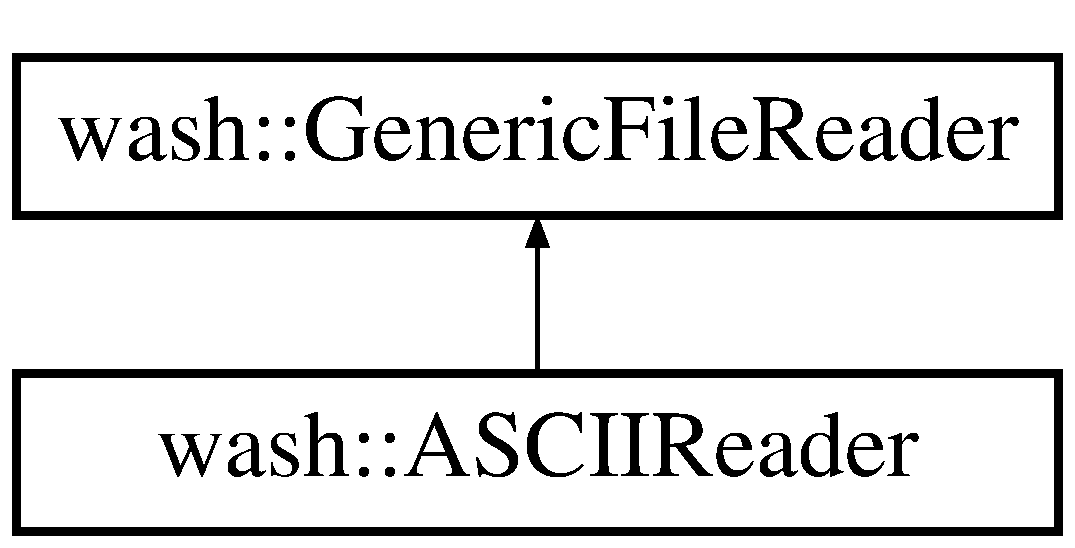
\includegraphics[height=2.000000cm]{classwash_1_1ASCIIReader}
\end{center}
\end{figure}
\subsection*{Public Member Functions}
\begin{DoxyCompactItemize}
\item 
\mbox{\Hypertarget{classwash_1_1ASCIIReader_ae9248e52a7bcf48e54b1cd63cebf3d42}\label{classwash_1_1ASCIIReader_ae9248e52a7bcf48e54b1cd63cebf3d42}} 
void {\bfseries read\+\_\+iteration} (const size\+\_\+t iteration\+\_\+number) const override
\end{DoxyCompactItemize}


The documentation for this class was generated from the following files\+:\begin{DoxyCompactItemize}
\item 
/dcs/20/u2002000/4th\+Year\+Project/wash/src/io/ascii.\+hpp\item 
/dcs/20/u2002000/4th\+Year\+Project/wash/src/io/\mbox{\hyperlink{read__ascii_8cpp}{read\+\_\+ascii.\+cpp}}\end{DoxyCompactItemize}

\hypertarget{classwash_1_1ASCIIWriter}{}\section{wash\+:\+:A\+S\+C\+I\+I\+Writer Class Reference}
\label{classwash_1_1ASCIIWriter}\index{wash\+::\+A\+S\+C\+I\+I\+Writer@{wash\+::\+A\+S\+C\+I\+I\+Writer}}
Inheritance diagram for wash\+:\+:A\+S\+C\+I\+I\+Writer\+:\begin{figure}[H]
\begin{center}
\leavevmode
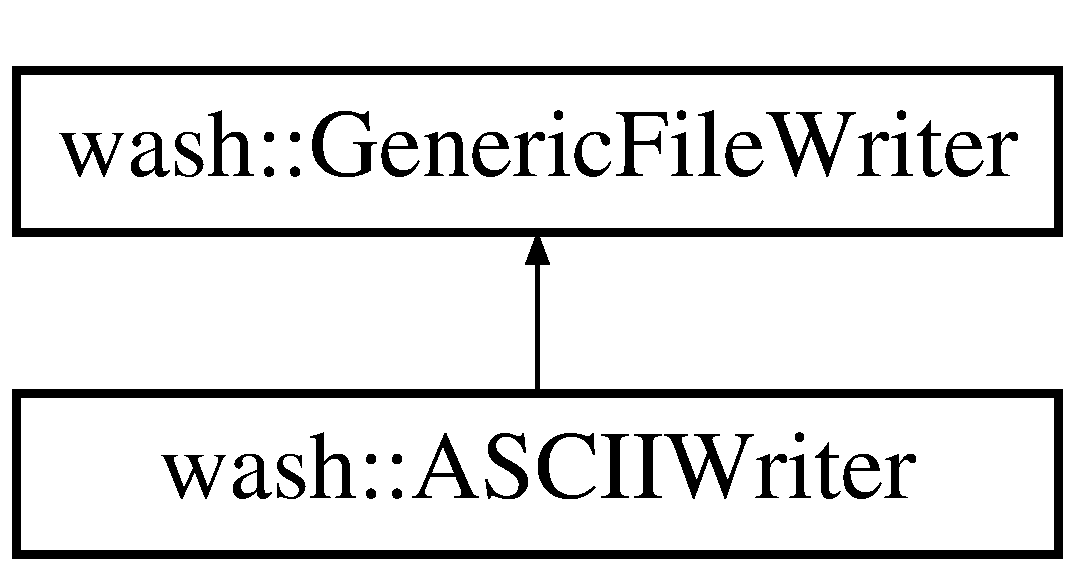
\includegraphics[height=2.000000cm]{classwash_1_1ASCIIWriter}
\end{center}
\end{figure}
\subsection*{Public Member Functions}
\begin{DoxyCompactItemize}
\item 
\mbox{\Hypertarget{classwash_1_1ASCIIWriter_ab6594fb85b025fe5ab21114be676a22b}\label{classwash_1_1ASCIIWriter_ab6594fb85b025fe5ab21114be676a22b}} 
void {\bfseries begin\+\_\+iteration} (const size\+\_\+t iterationc, const std\+::string path) override
\item 
\mbox{\Hypertarget{classwash_1_1ASCIIWriter_ae0d91c1d0a7af5dfb8d0e36b33b7d3c7}\label{classwash_1_1ASCIIWriter_ae0d91c1d0a7af5dfb8d0e36b33b7d3c7}} 
void {\bfseries write\+\_\+iteration\+\_\+attributes} () override
\item 
\mbox{\Hypertarget{classwash_1_1ASCIIWriter_add2c857439ee812ecb7ccd80459ed15a}\label{classwash_1_1ASCIIWriter_add2c857439ee812ecb7ccd80459ed15a}} 
void {\bfseries write\+\_\+file\+\_\+attributes} () override
\item 
\mbox{\Hypertarget{classwash_1_1ASCIIWriter_aaa3c025d6ec340208f804ad045c9b64a}\label{classwash_1_1ASCIIWriter_aaa3c025d6ec340208f804ad045c9b64a}} 
void {\bfseries write\+\_\+particle} () override
\item 
\mbox{\Hypertarget{classwash_1_1ASCIIWriter_a2614dfedb389b02f2cddfc2792ab769a}\label{classwash_1_1ASCIIWriter_a2614dfedb389b02f2cddfc2792ab769a}} 
void {\bfseries finish\+\_\+iteration} () override
\end{DoxyCompactItemize}


The documentation for this class was generated from the following files\+:\begin{DoxyCompactItemize}
\item 
/dcs/20/u2002000/4th\+Year\+Project/wash/io/ascii.\+hpp\item 
/dcs/20/u2002000/4th\+Year\+Project/wash/io/\mbox{\hyperlink{write__ascii_8cpp}{write\+\_\+ascii.\+cpp}}\end{DoxyCompactItemize}

\hypertarget{classFindWashFunctionAction}{}\section{Find\+Wash\+Function\+Action Class Reference}
\label{classFindWashFunctionAction}\index{Find\+Wash\+Function\+Action@{Find\+Wash\+Function\+Action}}
Inheritance diagram for Find\+Wash\+Function\+Action\+:\begin{figure}[H]
\begin{center}
\leavevmode
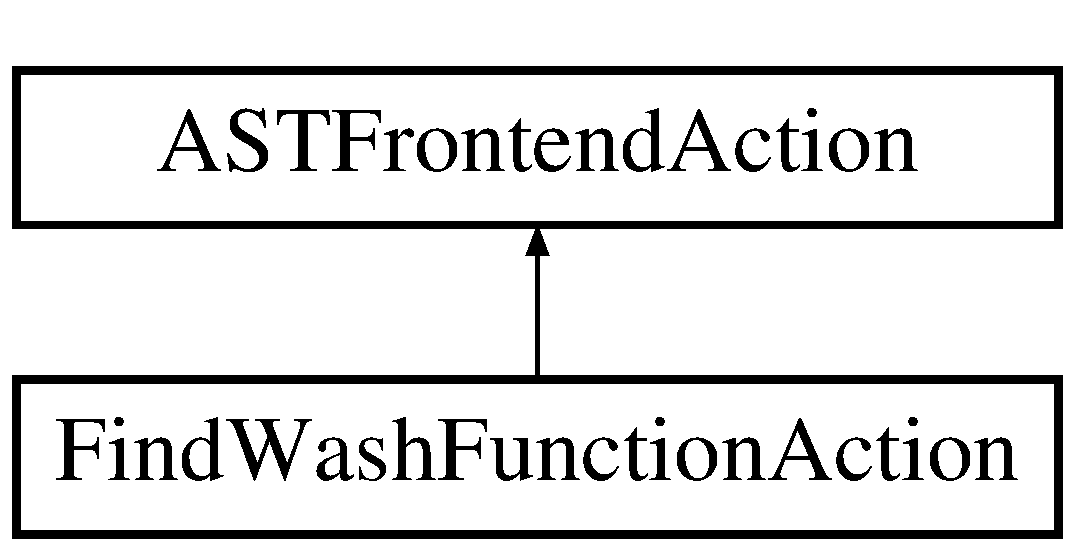
\includegraphics[height=2.000000cm]{classFindWashFunctionAction}
\end{center}
\end{figure}
\subsection*{Public Member Functions}
\begin{DoxyCompactItemize}
\item 
\mbox{\Hypertarget{classFindWashFunctionAction_a1e49f05e07b1794e456beb4afb203de5}\label{classFindWashFunctionAction_a1e49f05e07b1794e456beb4afb203de5}} 
std\+::unique\+\_\+ptr$<$ clang\+::\+A\+S\+T\+Consumer $>$ {\bfseries Create\+A\+S\+T\+Consumer} (clang\+::\+Compiler\+Instance \&Compiler, llvm\+::\+String\+Ref In\+File)
\end{DoxyCompactItemize}


The documentation for this class was generated from the following file\+:\begin{DoxyCompactItemize}
\item 
/dcs/20/u2002000/4th\+Year\+Project/wash/src/gen/\mbox{\hyperlink{finder__tool_8cpp}{finder\+\_\+tool.\+cpp}}\end{DoxyCompactItemize}

\hypertarget{classFindWashFunctionConsumer}{}\section{Find\+Wash\+Function\+Consumer Class Reference}
\label{classFindWashFunctionConsumer}\index{Find\+Wash\+Function\+Consumer@{Find\+Wash\+Function\+Consumer}}
Inheritance diagram for Find\+Wash\+Function\+Consumer\+:\begin{figure}[H]
\begin{center}
\leavevmode
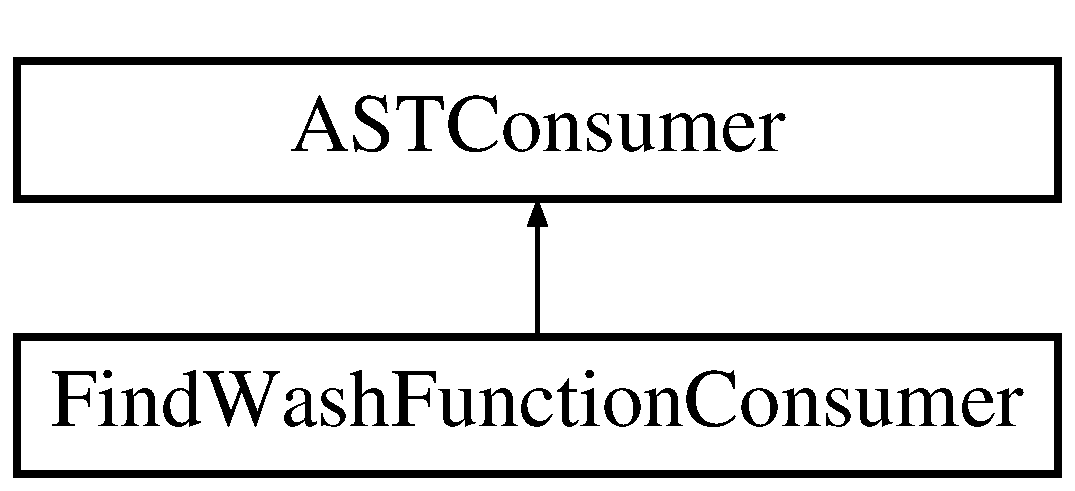
\includegraphics[height=2.000000cm]{classFindWashFunctionConsumer}
\end{center}
\end{figure}
\subsection*{Public Member Functions}
\begin{DoxyCompactItemize}
\item 
\mbox{\Hypertarget{classFindWashFunctionConsumer_a98780796544492f4124d6ae75a50f711}\label{classFindWashFunctionConsumer_a98780796544492f4124d6ae75a50f711}} 
{\bfseries Find\+Wash\+Function\+Consumer} (clang\+::\+A\+S\+T\+Context $\ast$Context)
\item 
\mbox{\Hypertarget{classFindWashFunctionConsumer_a31623a8aa3a9a74cee3fd73ebf53aec3}\label{classFindWashFunctionConsumer_a31623a8aa3a9a74cee3fd73ebf53aec3}} 
void {\bfseries Handle\+Translation\+Unit} (clang\+::\+A\+S\+T\+Context \&Context) override
\item 
\mbox{\Hypertarget{classFindWashFunctionConsumer_a3e833697a58085ed53f0407a3b82a64f}\label{classFindWashFunctionConsumer_a3e833697a58085ed53f0407a3b82a64f}} 
bool {\bfseries Handle\+Top\+Level\+Decl} (clang\+::\+Decl\+Group\+Ref DG) override
\end{DoxyCompactItemize}


The documentation for this class was generated from the following files\+:\begin{DoxyCompactItemize}
\item 
/dcs/20/u2002000/4th\+Year\+Project/wash/src/gen/\mbox{\hyperlink{finder_8hpp}{finder.\+hpp}}\item 
/dcs/20/u2002000/4th\+Year\+Project/wash/src/gen/\mbox{\hyperlink{finder_8cpp}{finder.\+cpp}}\end{DoxyCompactItemize}

\hypertarget{classFindWashFunctionsPlugin}{}\section{Find\+Wash\+Functions\+Plugin Class Reference}
\label{classFindWashFunctionsPlugin}\index{Find\+Wash\+Functions\+Plugin@{Find\+Wash\+Functions\+Plugin}}


Implements the plugin through using the already defined behaviour of the frontent action.  


Inheritance diagram for Find\+Wash\+Functions\+Plugin\+:\begin{figure}[H]
\begin{center}
\leavevmode
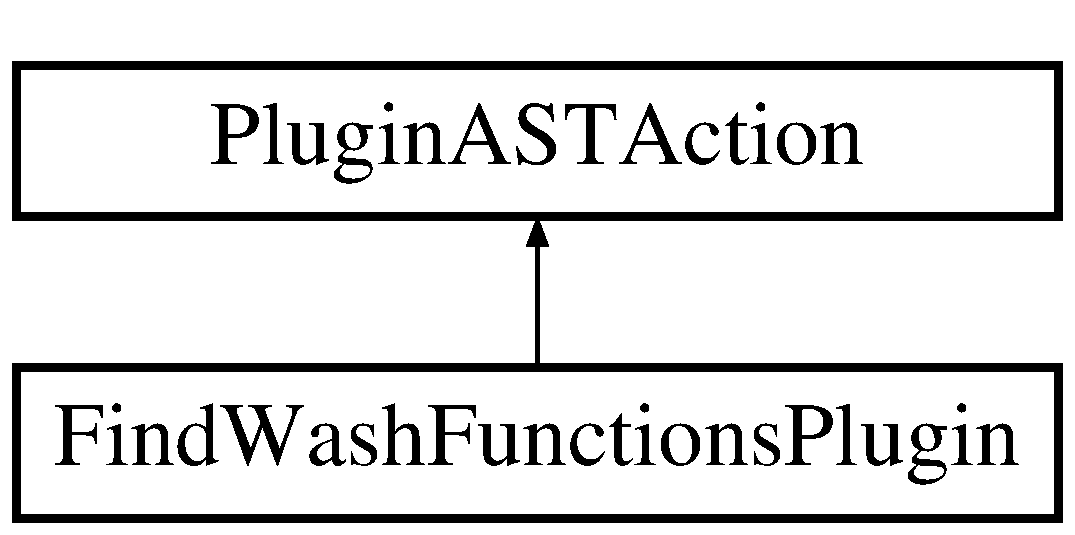
\includegraphics[height=2.000000cm]{classFindWashFunctionsPlugin}
\end{center}
\end{figure}
\subsection*{Public Member Functions}
\begin{DoxyCompactItemize}
\item 
\mbox{\Hypertarget{classFindWashFunctionsPlugin_acbaba39a9d96878d684361427c0d92ad}\label{classFindWashFunctionsPlugin_acbaba39a9d96878d684361427c0d92ad}} 
std\+::unique\+\_\+ptr$<$ clang\+::\+A\+S\+T\+Consumer $>$ {\bfseries Create\+A\+S\+T\+Consumer} (clang\+::\+Compiler\+Instance \&Compiler, llvm\+::\+String\+Ref In\+File) override
\item 
\mbox{\Hypertarget{classFindWashFunctionsPlugin_a5a26a021392c239258217236f1016a20}\label{classFindWashFunctionsPlugin_a5a26a021392c239258217236f1016a20}} 
bool \mbox{\hyperlink{classFindWashFunctionsPlugin_a5a26a021392c239258217236f1016a20}{Parse\+Args}} (const clang\+::\+Compiler\+Instance \&CI, const std\+::vector$<$ std\+::string $>$ \&args) override
\begin{DoxyCompactList}\small\item\em Allows the plugin to take in a set of arguments. \end{DoxyCompactList}\item 
\mbox{\Hypertarget{classFindWashFunctionsPlugin_a6c0b54d000be41e28df04e36bbde4561}\label{classFindWashFunctionsPlugin_a6c0b54d000be41e28df04e36bbde4561}} 
clang\+::\+Plugin\+A\+S\+T\+Action\+::\+Action\+Type \mbox{\hyperlink{classFindWashFunctionsPlugin_a6c0b54d000be41e28df04e36bbde4561}{get\+Action\+Type}} () override
\begin{DoxyCompactList}\small\item\em Sets when this plugin should be run. Before Main Action = Before Code Gen I believe. \end{DoxyCompactList}\end{DoxyCompactItemize}


\subsection{Detailed Description}
Implements the plugin through using the already defined behaviour of the frontent action. 

The documentation for this class was generated from the following file\+:\begin{DoxyCompactItemize}
\item 
/dcs/20/u2002000/4th\+Year\+Project/wash/src/gen/\mbox{\hyperlink{finder__plugin_8cpp}{finder\+\_\+plugin.\+cpp}}\end{DoxyCompactItemize}

\hypertarget{classFindWashFunctionVisitor}{}\section{Find\+Wash\+Function\+Visitor Class Reference}
\label{classFindWashFunctionVisitor}\index{Find\+Wash\+Function\+Visitor@{Find\+Wash\+Function\+Visitor}}
Inheritance diagram for Find\+Wash\+Function\+Visitor\+:\begin{figure}[H]
\begin{center}
\leavevmode
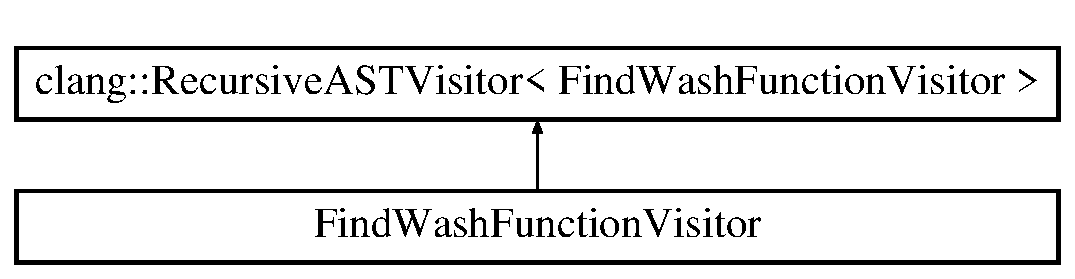
\includegraphics[height=2.000000cm]{classFindWashFunctionVisitor}
\end{center}
\end{figure}
\subsection*{Public Member Functions}
\begin{DoxyCompactItemize}
\item 
\mbox{\Hypertarget{classFindWashFunctionVisitor_a83067680ea5327ae0e11defa2a7febe7}\label{classFindWashFunctionVisitor_a83067680ea5327ae0e11defa2a7febe7}} 
{\bfseries Find\+Wash\+Function\+Visitor} (clang\+::\+A\+S\+T\+Context $\ast$Context)
\item 
\mbox{\Hypertarget{classFindWashFunctionVisitor_a4a2537acabc326871fa4b7ad80713704}\label{classFindWashFunctionVisitor_a4a2537acabc326871fa4b7ad80713704}} 
bool {\bfseries Visit\+Function\+Decl} (clang\+::\+Function\+Decl $\ast$Declaration)
\item 
\mbox{\Hypertarget{classFindWashFunctionVisitor_af5fd9befa463954aa1124fae02ed7098}\label{classFindWashFunctionVisitor_af5fd9befa463954aa1124fae02ed7098}} 
bool {\bfseries Visit\+Call\+Expr} (clang\+::\+Call\+Expr $\ast$Expression)
\end{DoxyCompactItemize}


The documentation for this class was generated from the following files\+:\begin{DoxyCompactItemize}
\item 
/dcs/20/u2002000/4th\+Year\+Project/wash/src/gen/\mbox{\hyperlink{finder_8hpp}{finder.\+hpp}}\item 
/dcs/20/u2002000/4th\+Year\+Project/wash/src/gen/\mbox{\hyperlink{finder_8cpp}{finder.\+cpp}}\end{DoxyCompactItemize}

\hypertarget{classwash_1_1ForceKernel}{}\section{wash\+:\+:Force\+Kernel Class Reference}
\label{classwash_1_1ForceKernel}\index{wash\+::\+Force\+Kernel@{wash\+::\+Force\+Kernel}}


Force \mbox{\hyperlink{classwash_1_1Kernel}{Kernel}} Class.  




{\ttfamily \#include $<$kernels.\+hpp$>$}

Inheritance diagram for wash\+:\+:Force\+Kernel\+:\begin{figure}[H]
\begin{center}
\leavevmode
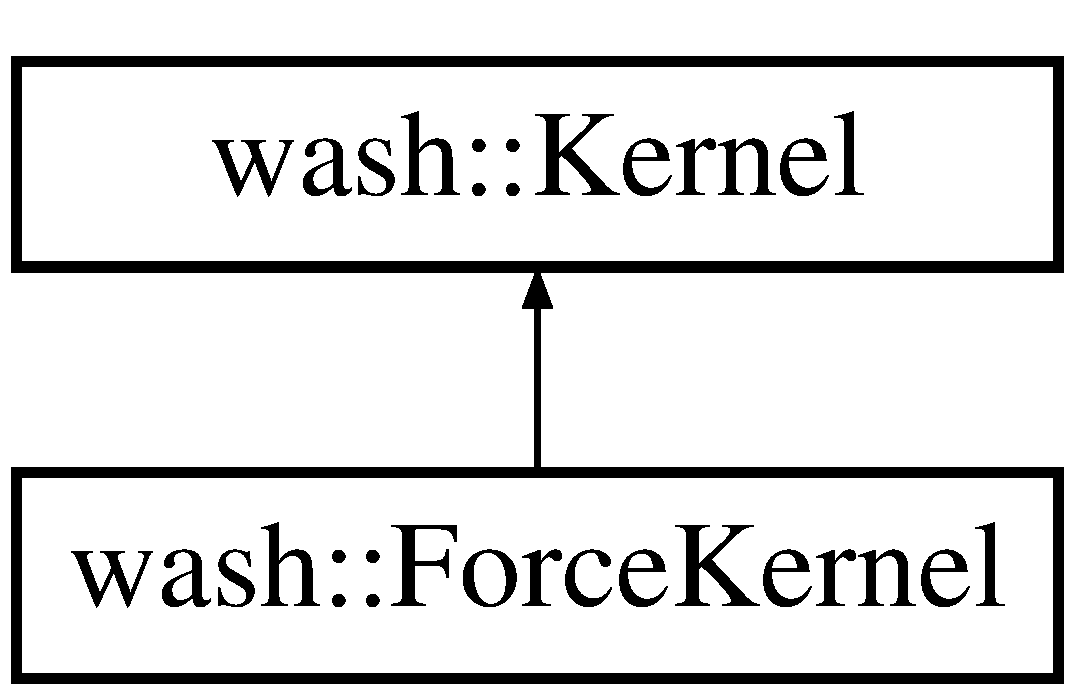
\includegraphics[height=2.000000cm]{classwash_1_1ForceKernel}
\end{center}
\end{figure}
\subsection*{Public Member Functions}
\begin{DoxyCompactItemize}
\item 
\mbox{\hyperlink{classwash_1_1ForceKernel_a5dd87d8036d74c210c51fb6aa97a3de8}{Force\+Kernel}} (const \mbox{\hyperlink{namespacewash_a3687ea698f8cb8c077d728e5d74de495}{Force\+FuncT}} func)
\item 
virtual void \mbox{\hyperlink{classwash_1_1ForceKernel_aa815514d4e9af5ebb056dbe8f1d5a720}{exec}} () const override
\end{DoxyCompactItemize}


\subsection{Detailed Description}
Force \mbox{\hyperlink{classwash_1_1Kernel}{Kernel}} Class. 

This kernel is used to update a force (or multiple forces) of a particle given its neighbours. 

\subsection{Constructor \& Destructor Documentation}
\mbox{\Hypertarget{classwash_1_1ForceKernel_a5dd87d8036d74c210c51fb6aa97a3de8}\label{classwash_1_1ForceKernel_a5dd87d8036d74c210c51fb6aa97a3de8}} 
\index{wash\+::\+Force\+Kernel@{wash\+::\+Force\+Kernel}!Force\+Kernel@{Force\+Kernel}}
\index{Force\+Kernel@{Force\+Kernel}!wash\+::\+Force\+Kernel@{wash\+::\+Force\+Kernel}}
\subsubsection{\texorpdfstring{Force\+Kernel()}{ForceKernel()}}
{\footnotesize\ttfamily wash\+::\+Force\+Kernel\+::\+Force\+Kernel (\begin{DoxyParamCaption}\item[{const \mbox{\hyperlink{namespacewash_a3687ea698f8cb8c077d728e5d74de495}{Force\+FuncT}}}]{func }\end{DoxyParamCaption})\hspace{0.3cm}{\ttfamily [inline]}}



\subsection{Member Function Documentation}
\mbox{\Hypertarget{classwash_1_1ForceKernel_aa815514d4e9af5ebb056dbe8f1d5a720}\label{classwash_1_1ForceKernel_aa815514d4e9af5ebb056dbe8f1d5a720}} 
\index{wash\+::\+Force\+Kernel@{wash\+::\+Force\+Kernel}!exec@{exec}}
\index{exec@{exec}!wash\+::\+Force\+Kernel@{wash\+::\+Force\+Kernel}}
\subsubsection{\texorpdfstring{exec()}{exec()}}
{\footnotesize\ttfamily void wash\+::\+Force\+Kernel\+::exec (\begin{DoxyParamCaption}{ }\end{DoxyParamCaption}) const\hspace{0.3cm}{\ttfamily [override]}, {\ttfamily [virtual]}}



Implements \mbox{\hyperlink{classwash_1_1Kernel_a0ec211840402ce975997b22136f16e39}{wash\+::\+Kernel}}.



The documentation for this class was generated from the following files\+:\begin{DoxyCompactItemize}
\item 
/dcs/20/u2002000/4th\+Year\+Project/wash/include/\mbox{\hyperlink{kernels_8hpp}{kernels.\+hpp}}\item 
/dcs/20/u2002000/4th\+Year\+Project/wash/src/impl/cstone/\mbox{\hyperlink{cstone_2kernels_8cpp}{kernels.\+cpp}}\end{DoxyCompactItemize}

\hypertarget{classwash_1_1GenericFileReader}{}\section{wash\+:\+:Generic\+File\+Reader Class Reference}
\label{classwash_1_1GenericFileReader}\index{wash\+::\+Generic\+File\+Reader@{wash\+::\+Generic\+File\+Reader}}
Inheritance diagram for wash\+:\+:Generic\+File\+Reader\+:\begin{figure}[H]
\begin{center}
\leavevmode
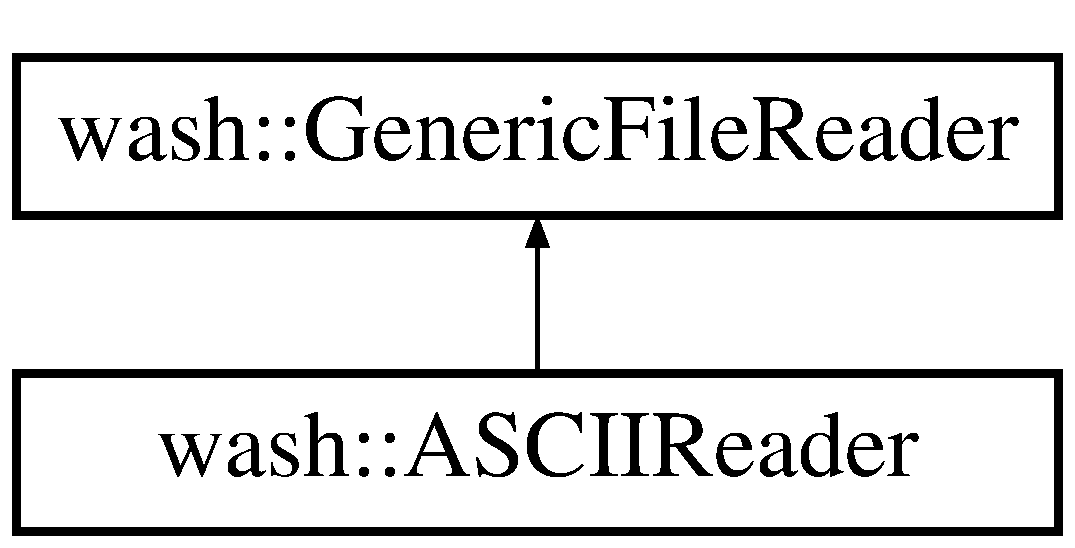
\includegraphics[height=2.000000cm]{classwash_1_1GenericFileReader}
\end{center}
\end{figure}
\subsection*{Public Member Functions}
\begin{DoxyCompactItemize}
\item 
\mbox{\Hypertarget{classwash_1_1GenericFileReader_a4be5668152706252a4d5759568cf4062}\label{classwash_1_1GenericFileReader_a4be5668152706252a4d5759568cf4062}} 
virtual void {\bfseries read\+\_\+iteration} (const size\+\_\+t iteration\+\_\+number) const =0
\end{DoxyCompactItemize}


The documentation for this class was generated from the following file\+:\begin{DoxyCompactItemize}
\item 
/dcs/20/u2002000/4th\+Year\+Project/wash/src/io/io.\+hpp\end{DoxyCompactItemize}

\hypertarget{classwash_1_1GenericFileWriter}{}\section{wash\+:\+:Generic\+File\+Writer Class Reference}
\label{classwash_1_1GenericFileWriter}\index{wash\+::\+Generic\+File\+Writer@{wash\+::\+Generic\+File\+Writer}}
Inheritance diagram for wash\+:\+:Generic\+File\+Writer\+:\begin{figure}[H]
\begin{center}
\leavevmode
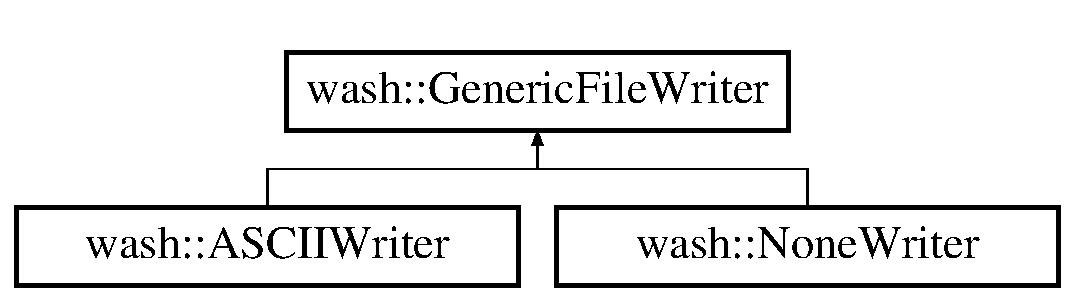
\includegraphics[height=2.000000cm]{classwash_1_1GenericFileWriter}
\end{center}
\end{figure}
\subsection*{Public Member Functions}
\begin{DoxyCompactItemize}
\item 
\mbox{\Hypertarget{classwash_1_1GenericFileWriter_aae09bd9ec13abb5c3935062e79338fef}\label{classwash_1_1GenericFileWriter_aae09bd9ec13abb5c3935062e79338fef}} 
virtual void {\bfseries write\+\_\+iteration} (const size\+\_\+t iterationc, const std\+::string path) const =0
\end{DoxyCompactItemize}


The documentation for this class was generated from the following file\+:\begin{DoxyCompactItemize}
\item 
/dcs/20/u2002000/4th\+Year\+Project/wash/src/io/io.\+hpp\end{DoxyCompactItemize}

\hypertarget{classwash_1_1IOManager}{}\section{wash\+:\+:I\+O\+Manager Class Reference}
\label{classwash_1_1IOManager}\index{wash\+::\+I\+O\+Manager@{wash\+::\+I\+O\+Manager}}


Manages the IO options for the simulation.  




{\ttfamily \#include $<$io.\+hpp$>$}

\subsection*{Public Member Functions}
\begin{DoxyCompactItemize}
\item 
\mbox{\Hypertarget{classwash_1_1IOManager_a700c9e0c1b3f90e408012b7b97fdf74c}\label{classwash_1_1IOManager_a700c9e0c1b3f90e408012b7b97fdf74c}} 
{\bfseries I\+O\+Manager} (const std\+::string format)
\item 
\mbox{\Hypertarget{classwash_1_1IOManager_ae2b51434752a46f631c9c20ecb99e5d2}\label{classwash_1_1IOManager_ae2b51434752a46f631c9c20ecb99e5d2}} 
{\bfseries I\+O\+Manager} (const std\+::string format, const size\+\_\+t output\+\_\+nth)
\item 
\mbox{\Hypertarget{classwash_1_1IOManager_a7c04519d80a8e1ff53d58a6a7d412209}\label{classwash_1_1IOManager_a7c04519d80a8e1ff53d58a6a7d412209}} 
void {\bfseries set\+\_\+path} (std\+::string simulation\+\_\+name, std\+::string output\+\_\+file\+\_\+name)
\item 
\mbox{\Hypertarget{classwash_1_1IOManager_a061951b9d8f6c47e625e0bbf27507b01}\label{classwash_1_1IOManager_a061951b9d8f6c47e625e0bbf27507b01}} 
const std\+::string {\bfseries get\+\_\+path} () const
\item 
void \mbox{\hyperlink{classwash_1_1IOManager_a37c0150160a8e7f4e97951469d9abb30}{handle\+\_\+iteration}} (size\+\_\+t iteration) const
\begin{DoxyCompactList}\small\item\em Dispatches an iteration call to the writer based on the iteration number. \end{DoxyCompactList}\item 
void \mbox{\hyperlink{classwash_1_1IOManager_ae635581c17822a8f18c228952000e6cc}{write\+\_\+timings}} (const std\+::string \&event\+\_\+name, const int tag, const int64\+\_\+t time\+\_\+taken) const
\begin{DoxyCompactList}\small\item\em Write a timing even out to a file. \end{DoxyCompactList}\end{DoxyCompactItemize}


\subsection{Detailed Description}
Manages the IO options for the simulation. 

\subsection{Member Function Documentation}
\mbox{\Hypertarget{classwash_1_1IOManager_a37c0150160a8e7f4e97951469d9abb30}\label{classwash_1_1IOManager_a37c0150160a8e7f4e97951469d9abb30}} 
\index{wash\+::\+I\+O\+Manager@{wash\+::\+I\+O\+Manager}!handle\+\_\+iteration@{handle\+\_\+iteration}}
\index{handle\+\_\+iteration@{handle\+\_\+iteration}!wash\+::\+I\+O\+Manager@{wash\+::\+I\+O\+Manager}}
\subsubsection{\texorpdfstring{handle\+\_\+iteration()}{handle\_iteration()}}
{\footnotesize\ttfamily void wash\+::\+I\+O\+Manager\+::handle\+\_\+iteration (\begin{DoxyParamCaption}\item[{size\+\_\+t}]{iteration }\end{DoxyParamCaption}) const\hspace{0.3cm}{\ttfamily [inline]}}



Dispatches an iteration call to the writer based on the iteration number. 


\begin{DoxyParams}{Parameters}
{\em iteration} & \\
\hline
\end{DoxyParams}
\mbox{\Hypertarget{classwash_1_1IOManager_ae635581c17822a8f18c228952000e6cc}\label{classwash_1_1IOManager_ae635581c17822a8f18c228952000e6cc}} 
\index{wash\+::\+I\+O\+Manager@{wash\+::\+I\+O\+Manager}!write\+\_\+timings@{write\+\_\+timings}}
\index{write\+\_\+timings@{write\+\_\+timings}!wash\+::\+I\+O\+Manager@{wash\+::\+I\+O\+Manager}}
\subsubsection{\texorpdfstring{write\+\_\+timings()}{write\_timings()}}
{\footnotesize\ttfamily void wash\+::\+I\+O\+Manager\+::write\+\_\+timings (\begin{DoxyParamCaption}\item[{const std\+::string \&}]{event\+\_\+name,  }\item[{const int}]{tag,  }\item[{const int64\+\_\+t}]{time\+\_\+taken }\end{DoxyParamCaption}) const\hspace{0.3cm}{\ttfamily [inline]}}



Write a timing even out to a file. 


\begin{DoxyParams}{Parameters}
{\em event\+\_\+name} & \\
\hline
{\em time\+\_\+taken} & \\
\hline
\end{DoxyParams}


The documentation for this class was generated from the following file\+:\begin{DoxyCompactItemize}
\item 
/dcs/20/u2002000/4th\+Year\+Project/wash/src/io/io.\+hpp\end{DoxyCompactItemize}

\hypertarget{classwash_1_1Kernel}{}\section{wash\+:\+:Kernel Class Reference}
\label{classwash_1_1Kernel}\index{wash\+::\+Kernel@{wash\+::\+Kernel}}


Parent \mbox{\hyperlink{classwash_1_1Kernel}{Kernel}} Class.  




{\ttfamily \#include $<$kernels.\+hpp$>$}

Inheritance diagram for wash\+:\+:Kernel\+:\begin{figure}[H]
\begin{center}
\leavevmode
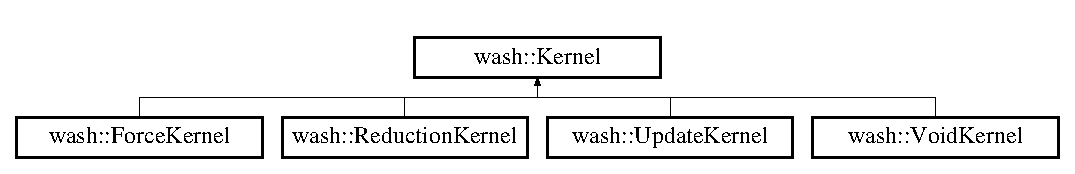
\includegraphics[height=1.891892cm]{classwash_1_1Kernel}
\end{center}
\end{figure}
\subsection*{Public Member Functions}
\begin{DoxyCompactItemize}
\item 
\mbox{\Hypertarget{classwash_1_1Kernel_a0ec211840402ce975997b22136f16e39}\label{classwash_1_1Kernel_a0ec211840402ce975997b22136f16e39}} 
virtual void {\bfseries exec} () const =0
\end{DoxyCompactItemize}


\subsection{Detailed Description}
Parent \mbox{\hyperlink{classwash_1_1Kernel}{Kernel}} Class. 

A \mbox{\hyperlink{classwash_1_1Kernel}{Kernel}} in Wa\+SH can take one of four forms, which all inherit from this class. 

The documentation for this class was generated from the following file\+:\begin{DoxyCompactItemize}
\item 
/dcs/20/u2002000/4th\+Year\+Project/wash/include/kernels.\+hpp\end{DoxyCompactItemize}

\hypertarget{classLoopPrinter}{}\section{Loop\+Printer Class Reference}
\label{classLoopPrinter}\index{Loop\+Printer@{Loop\+Printer}}
Inheritance diagram for Loop\+Printer\+:\begin{figure}[H]
\begin{center}
\leavevmode
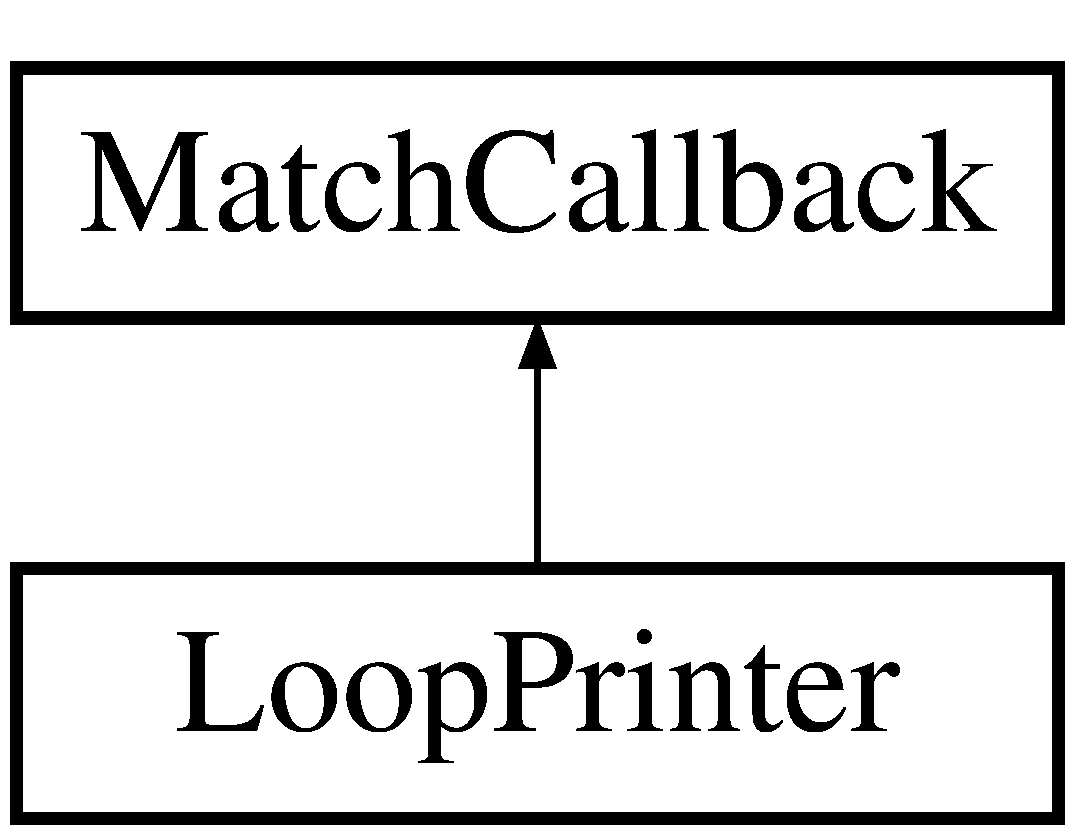
\includegraphics[height=2.000000cm]{classLoopPrinter}
\end{center}
\end{figure}
\subsection*{Public Member Functions}
\begin{DoxyCompactItemize}
\item 
\mbox{\Hypertarget{classLoopPrinter_ae59e0b9aaac96e2e564706ff060e0c57}\label{classLoopPrinter_ae59e0b9aaac96e2e564706ff060e0c57}} 
virtual void {\bfseries run} (const Match\+Finder\+::\+Match\+Result \&Result)
\end{DoxyCompactItemize}


The documentation for this class was generated from the following file\+:\begin{DoxyCompactItemize}
\item 
/dcs/20/u2002000/4th\+Year\+Project/wash/src/ws2st/refactor.\+cpp\end{DoxyCompactItemize}

\hypertarget{structbetter__enums_1_1map}{}\section{better\+\_\+enums\+:\+:map$<$ Enum, T, Compare $>$ Struct Template Reference}
\label{structbetter__enums_1_1map}\index{better\+\_\+enums\+::map$<$ Enum, T, Compare $>$@{better\+\_\+enums\+::map$<$ Enum, T, Compare $>$}}
\subsection*{Public Types}
\begin{DoxyCompactItemize}
\item 
\mbox{\Hypertarget{structbetter__enums_1_1map_a225f81223779091e6761c74c766d7db1}\label{structbetter__enums_1_1map_a225f81223779091e6761c74c766d7db1}} 
typedef T($\ast$ {\bfseries function}) (Enum)
\end{DoxyCompactItemize}
\subsection*{Public Member Functions}
\begin{DoxyCompactItemize}
\item 
\mbox{\Hypertarget{structbetter__enums_1_1map_a5010e83ee9aa33e273832f344a7ffe10}\label{structbetter__enums_1_1map_a5010e83ee9aa33e273832f344a7ffe10}} 
B\+E\+T\+T\+E\+R\+\_\+\+E\+N\+U\+M\+S\+\_\+\+C\+O\+N\+S\+T\+E\+X\+P\+R\+\_\+ {\bfseries map} (function f)
\item 
\mbox{\Hypertarget{structbetter__enums_1_1map_afd371738df1b327d042a1bfe6938d92d}\label{structbetter__enums_1_1map_afd371738df1b327d042a1bfe6938d92d}} 
B\+E\+T\+T\+E\+R\+\_\+\+E\+N\+U\+M\+S\+\_\+\+C\+O\+N\+S\+T\+E\+X\+P\+R\+\_\+ T {\bfseries from\+\_\+enum} (Enum value) const
\item 
\mbox{\Hypertarget{structbetter__enums_1_1map_a0369a139acd93f5991103a2d5f3eacf9}\label{structbetter__enums_1_1map_a0369a139acd93f5991103a2d5f3eacf9}} 
B\+E\+T\+T\+E\+R\+\_\+\+E\+N\+U\+M\+S\+\_\+\+C\+O\+N\+S\+T\+E\+X\+P\+R\+\_\+ T {\bfseries operator\mbox{[}$\,$\mbox{]}} (Enum value) const
\item 
\mbox{\Hypertarget{structbetter__enums_1_1map_a18ad2328a67af6d866e2fbc16b890ece}\label{structbetter__enums_1_1map_a18ad2328a67af6d866e2fbc16b890ece}} 
B\+E\+T\+T\+E\+R\+\_\+\+E\+N\+U\+M\+S\+\_\+\+C\+O\+N\+S\+T\+E\+X\+P\+R\+\_\+ Enum {\bfseries to\+\_\+enum} (T value) const
\item 
\mbox{\Hypertarget{structbetter__enums_1_1map_a4191ed97b5cbb98022e5dd8b6f6d5b45}\label{structbetter__enums_1_1map_a4191ed97b5cbb98022e5dd8b6f6d5b45}} 
B\+E\+T\+T\+E\+R\+\_\+\+E\+N\+U\+M\+S\+\_\+\+C\+O\+N\+S\+T\+E\+X\+P\+R\+\_\+ \mbox{\hyperlink{structbetter__enums_1_1optional}{optional}}$<$ Enum $>$ {\bfseries to\+\_\+enum\+\_\+nothrow} (T value, size\+\_\+t index=0) const
\end{DoxyCompactItemize}


The documentation for this struct was generated from the following file\+:\begin{DoxyCompactItemize}
\item 
/dcs/20/u2002000/4th\+Year\+Project/wash/src/wash/enum.\+h\end{DoxyCompactItemize}

\hypertarget{structbetter__enums_1_1map__compare}{}\section{better\+\_\+enums\+:\+:map\+\_\+compare$<$ T $>$ Struct Template Reference}
\label{structbetter__enums_1_1map__compare}\index{better\+\_\+enums\+::map\+\_\+compare$<$ T $>$@{better\+\_\+enums\+::map\+\_\+compare$<$ T $>$}}
\subsection*{Static Public Member Functions}
\begin{DoxyCompactItemize}
\item 
\mbox{\Hypertarget{structbetter__enums_1_1map__compare_acc484428961e669d7f3e6ac67e86aa52}\label{structbetter__enums_1_1map__compare_acc484428961e669d7f3e6ac67e86aa52}} 
static B\+E\+T\+T\+E\+R\+\_\+\+E\+N\+U\+M\+S\+\_\+\+C\+O\+N\+S\+T\+E\+X\+P\+R\+\_\+ bool {\bfseries less} (const T \&a, const T \&b)
\end{DoxyCompactItemize}


The documentation for this struct was generated from the following file\+:\begin{DoxyCompactItemize}
\item 
/dcs/20/u2002000/4th\+Year\+Project/wash/src/wash/enum.\+h\end{DoxyCompactItemize}

\hypertarget{structbetter__enums_1_1map__compare_3_01const_01char_01_5_01_4}{}\section{better\+\_\+enums\+:\+:map\+\_\+compare$<$ const char $\ast$ $>$ Struct Template Reference}
\label{structbetter__enums_1_1map__compare_3_01const_01char_01_5_01_4}\index{better\+\_\+enums\+::map\+\_\+compare$<$ const char $\ast$ $>$@{better\+\_\+enums\+::map\+\_\+compare$<$ const char $\ast$ $>$}}
\subsection*{Static Public Member Functions}
\begin{DoxyCompactItemize}
\item 
\mbox{\Hypertarget{structbetter__enums_1_1map__compare_3_01const_01char_01_5_01_4_a4ad056e5d61495762399c88344f1ce72}\label{structbetter__enums_1_1map__compare_3_01const_01char_01_5_01_4_a4ad056e5d61495762399c88344f1ce72}} 
static B\+E\+T\+T\+E\+R\+\_\+\+E\+N\+U\+M\+S\+\_\+\+C\+O\+N\+S\+T\+E\+X\+P\+R\+\_\+ bool {\bfseries less} (const char $\ast$a, const char $\ast$b)
\end{DoxyCompactItemize}


The documentation for this struct was generated from the following file\+:\begin{DoxyCompactItemize}
\item 
/dcs/20/u2002000/4th\+Year\+Project/wash/src/wash/enum.\+h\end{DoxyCompactItemize}

\hypertarget{structbetter__enums_1_1map__compare_3_01const_01wchar__t_01_5_01_4}{}\section{better\+\_\+enums\+:\+:map\+\_\+compare$<$ const wchar\+\_\+t $\ast$ $>$ Struct Template Reference}
\label{structbetter__enums_1_1map__compare_3_01const_01wchar__t_01_5_01_4}\index{better\+\_\+enums\+::map\+\_\+compare$<$ const wchar\+\_\+t $\ast$ $>$@{better\+\_\+enums\+::map\+\_\+compare$<$ const wchar\+\_\+t $\ast$ $>$}}
\subsection*{Static Public Member Functions}
\begin{DoxyCompactItemize}
\item 
\mbox{\Hypertarget{structbetter__enums_1_1map__compare_3_01const_01wchar__t_01_5_01_4_a3d92f104915178f31373c48579a2a9d8}\label{structbetter__enums_1_1map__compare_3_01const_01wchar__t_01_5_01_4_a3d92f104915178f31373c48579a2a9d8}} 
static B\+E\+T\+T\+E\+R\+\_\+\+E\+N\+U\+M\+S\+\_\+\+C\+O\+N\+S\+T\+E\+X\+P\+R\+\_\+ bool {\bfseries less} (const wchar\+\_\+t $\ast$a, const wchar\+\_\+t $\ast$b)
\end{DoxyCompactItemize}


The documentation for this struct was generated from the following file\+:\begin{DoxyCompactItemize}
\item 
/dcs/20/u2002000/4th\+Year\+Project/wash/src/wash/enum.\+h\end{DoxyCompactItemize}

\hypertarget{classwash_1_1NoneReader}{}\section{wash\+:\+:None\+Reader Class Reference}
\label{classwash_1_1NoneReader}\index{wash\+::\+None\+Reader@{wash\+::\+None\+Reader}}
Inheritance diagram for wash\+:\+:None\+Reader\+:\begin{figure}[H]
\begin{center}
\leavevmode
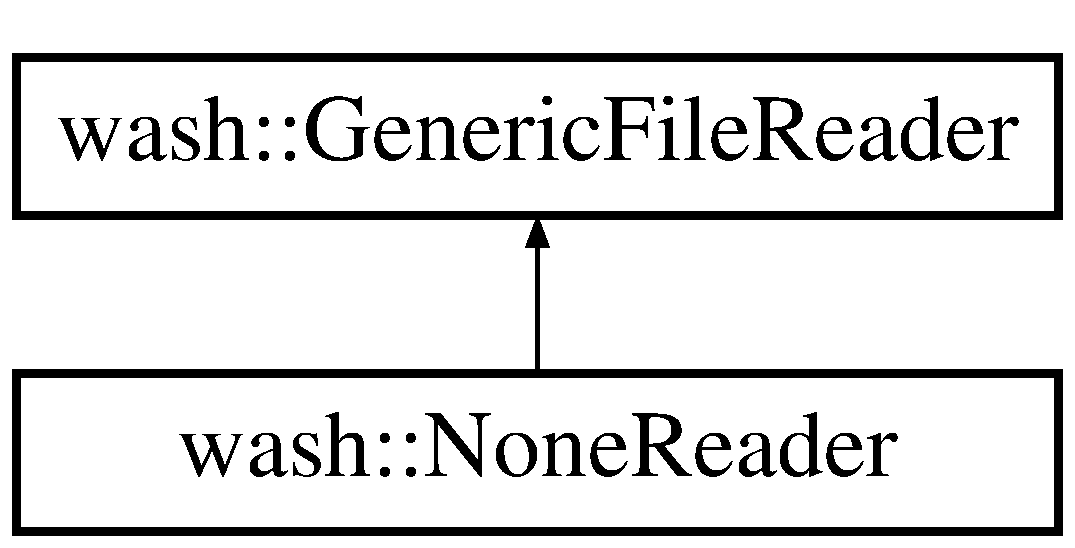
\includegraphics[height=2.000000cm]{classwash_1_1NoneReader}
\end{center}
\end{figure}
\subsection*{Public Member Functions}
\begin{DoxyCompactItemize}
\item 
\mbox{\Hypertarget{classwash_1_1NoneReader_aaaa9a5d1fe678c4feea3b33c1b14db4b}\label{classwash_1_1NoneReader_aaaa9a5d1fe678c4feea3b33c1b14db4b}} 
void {\bfseries read\+\_\+iteration} (const size\+\_\+t iteration\+\_\+number) const override
\end{DoxyCompactItemize}


The documentation for this class was generated from the following file\+:\begin{DoxyCompactItemize}
\item 
/dcs/20/u2002000/4th\+Year\+Project/wash/src/io/none.\+hpp\end{DoxyCompactItemize}

\hypertarget{classwash_1_1NoneWriter}{}\section{wash\+:\+:None\+Writer Class Reference}
\label{classwash_1_1NoneWriter}\index{wash\+::\+None\+Writer@{wash\+::\+None\+Writer}}
Inheritance diagram for wash\+:\+:None\+Writer\+:\begin{figure}[H]
\begin{center}
\leavevmode
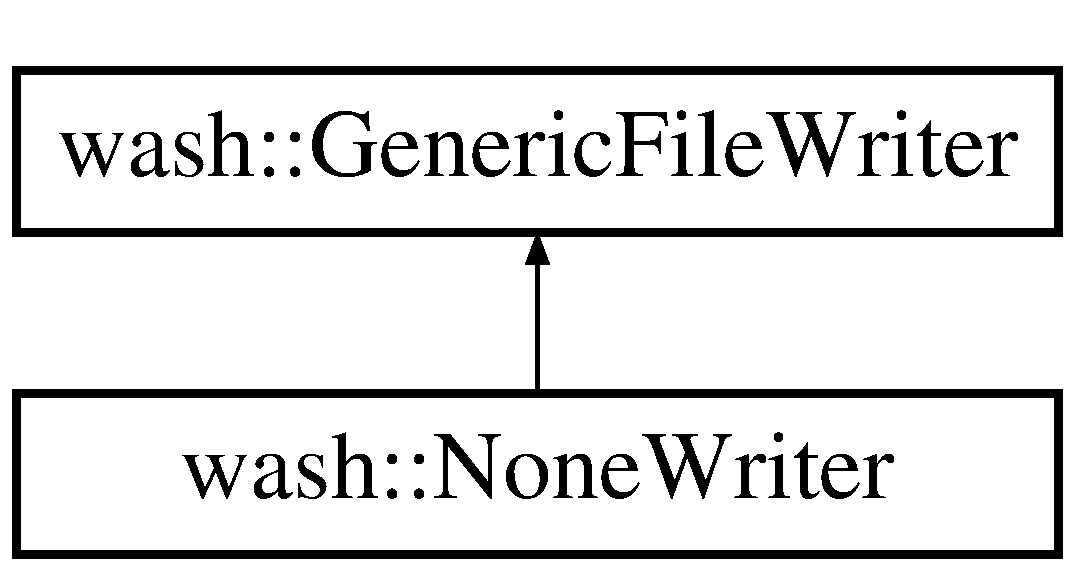
\includegraphics[height=2.000000cm]{classwash_1_1NoneWriter}
\end{center}
\end{figure}
\subsection*{Public Member Functions}
\begin{DoxyCompactItemize}
\item 
\mbox{\Hypertarget{classwash_1_1NoneWriter_a0c7980e62b349a3d883a75a673d687ca}\label{classwash_1_1NoneWriter_a0c7980e62b349a3d883a75a673d687ca}} 
void {\bfseries write\+\_\+iteration} (const size\+\_\+t iterationc, const std\+::string path) const override
\end{DoxyCompactItemize}


The documentation for this class was generated from the following file\+:\begin{DoxyCompactItemize}
\item 
/dcs/20/u2002000/4th\+Year\+Project/wash/src/io/none.\+hpp\end{DoxyCompactItemize}

\hypertarget{structbetter__enums_1_1optional}{}\section{better\+\_\+enums\+:\+:optional$<$ T $>$ Struct Template Reference}
\label{structbetter__enums_1_1optional}\index{better\+\_\+enums\+::optional$<$ T $>$@{better\+\_\+enums\+::optional$<$ T $>$}}
\subsection*{Public Member Functions}
\begin{DoxyCompactItemize}
\item 
\mbox{\Hypertarget{structbetter__enums_1_1optional_a893399829eb6dbdf7c8eb385b2ec464d}\label{structbetter__enums_1_1optional_a893399829eb6dbdf7c8eb385b2ec464d}} 
B\+E\+T\+T\+E\+R\+\_\+\+E\+N\+U\+M\+S\+\_\+\+C\+O\+N\+S\+T\+E\+X\+P\+R\+\_\+ {\bfseries optional} (T v)
\item 
\mbox{\Hypertarget{structbetter__enums_1_1optional_ac112a6e38895da91c4a5a96ee1a8460e}\label{structbetter__enums_1_1optional_ac112a6e38895da91c4a5a96ee1a8460e}} 
B\+E\+T\+T\+E\+R\+\_\+\+E\+N\+U\+M\+S\+\_\+\+C\+O\+N\+S\+T\+E\+X\+P\+R\+\_\+ const T \& {\bfseries operator$\ast$} () const
\item 
\mbox{\Hypertarget{structbetter__enums_1_1optional_a0eba3de653c3dbaa047e753a42fd59e1}\label{structbetter__enums_1_1optional_a0eba3de653c3dbaa047e753a42fd59e1}} 
B\+E\+T\+T\+E\+R\+\_\+\+E\+N\+U\+M\+S\+\_\+\+C\+O\+N\+S\+T\+E\+X\+P\+R\+\_\+ const T $\ast$ {\bfseries operator-\/$>$} () const
\item 
\mbox{\Hypertarget{structbetter__enums_1_1optional_a48429aab0bf3d616df7431a1871e2f75}\label{structbetter__enums_1_1optional_a48429aab0bf3d616df7431a1871e2f75}} 
B\+E\+T\+T\+E\+R\+\_\+\+E\+N\+U\+M\+S\+\_\+\+C\+O\+N\+S\+T\+E\+X\+P\+R\+\_\+ {\bfseries operator bool} () const
\item 
\mbox{\Hypertarget{structbetter__enums_1_1optional_afd33f8c0b31edbbc8db640a403899363}\label{structbetter__enums_1_1optional_afd33f8c0b31edbbc8db640a403899363}} 
B\+E\+T\+T\+E\+R\+\_\+\+E\+N\+U\+M\+S\+\_\+\+C\+O\+N\+S\+T\+E\+X\+P\+R\+\_\+ const T \& {\bfseries value} () const
\end{DoxyCompactItemize}


The documentation for this struct was generated from the following file\+:\begin{DoxyCompactItemize}
\item 
/dcs/20/u2002000/4th\+Year\+Project/wash/src/wash/enum.\+h\end{DoxyCompactItemize}

\hypertarget{classwash_1_1Particle}{}\section{wash\+:\+:Particle Class Reference}
\label{classwash_1_1Particle}\index{wash\+::\+Particle@{wash\+::\+Particle}}


{\ttfamily \#include $<$particle.\+hpp$>$}

\subsection*{Public Member Functions}
\begin{DoxyCompactItemize}
\item 
\mbox{\hyperlink{classwash_1_1Particle_a72131cdf3fdbcada383d81604fd49503}{Particle}} (const unsigned local\+\_\+idx)
\begin{DoxyCompactList}\small\item\em T\+O\+DO\+: see if this works if it\textquotesingle{}s a glocal spec defined flag rather than in just one file? \end{DoxyCompactList}\item 
unsigned \mbox{\hyperlink{classwash_1_1Particle_aef9f2814cc392598de7756e1046fea67}{get\+\_\+id}} () const
\begin{DoxyCompactList}\small\item\em Returns the global ID of the particle. \end{DoxyCompactList}\item 
double \mbox{\hyperlink{classwash_1_1Particle_a8c0ce3f48b189fd8550c3bfab17eec68}{get\+\_\+density}} () const
\item 
void \mbox{\hyperlink{classwash_1_1Particle_a6416678dd509c16c2933d315b6ae6156}{set\+\_\+density}} (const double \mbox{\hyperlink{3d__fluid__sim_2fluid__sim_8cpp_a140d94d7edb97c062961056d1926a2db}{density}})
\item 
double \mbox{\hyperlink{classwash_1_1Particle_a7d8d11b3e4855e66e62ee58b4270cdc1}{get\+\_\+mass}} () const
\item 
void \mbox{\hyperlink{classwash_1_1Particle_a9151ed34c880f63f062381076834223e}{set\+\_\+mass}} (const double mass)
\item 
double \mbox{\hyperlink{classwash_1_1Particle_aab02f56502c6521382cf7a7320abc341}{get\+\_\+smoothing\+\_\+length}} () const
\item 
void \mbox{\hyperlink{classwash_1_1Particle_a15892a4346c05de955f91087dc88786d}{set\+\_\+smoothing\+\_\+length}} (const double smoothing\+\_\+length)
\item 
\mbox{\hyperlink{namespacewash_ab2cbbc37941b733095c9225b49b4cad9}{Simulation\+VecT}} \mbox{\hyperlink{classwash_1_1Particle_a9d222d453d640cf629ee8dfbee6b43c2}{get\+\_\+pos}} () const
\item 
void \mbox{\hyperlink{classwash_1_1Particle_af06835533935c04e594c258a7dcdd1ef}{set\+\_\+pos}} (const \mbox{\hyperlink{namespacewash_ab2cbbc37941b733095c9225b49b4cad9}{Simulation\+VecT}} pos)
\item 
\mbox{\hyperlink{namespacewash_ab2cbbc37941b733095c9225b49b4cad9}{Simulation\+VecT}} \mbox{\hyperlink{classwash_1_1Particle_a890d0f1467225393e385872b0c98b974}{get\+\_\+vel}} () const
\item 
void \mbox{\hyperlink{classwash_1_1Particle_a4755365883cfd62117ebe74fe44d35e0}{set\+\_\+vel}} (const \mbox{\hyperlink{namespacewash_ab2cbbc37941b733095c9225b49b4cad9}{Simulation\+VecT}} vel)
\item 
\mbox{\hyperlink{namespacewash_ab2cbbc37941b733095c9225b49b4cad9}{Simulation\+VecT}} \mbox{\hyperlink{classwash_1_1Particle_afb8c9dce2692cdfab61a3a87fde50610}{get\+\_\+acc}} () const
\item 
void \mbox{\hyperlink{classwash_1_1Particle_a395e095de0b2af7dfc925bedef2090a1}{set\+\_\+acc}} (const \mbox{\hyperlink{namespacewash_ab2cbbc37941b733095c9225b49b4cad9}{Simulation\+VecT}} acc)
\item 
double \mbox{\hyperlink{classwash_1_1Particle_ab42a162b41a4e8cf6212bd9c43f3a0cf}{get\+\_\+force\+\_\+scalar}} (const std\+::string \&force) const
\item 
void \mbox{\hyperlink{classwash_1_1Particle_a2c3038c8eac34e371922bcf1ab79b8ca}{set\+\_\+force\+\_\+scalar}} (const std\+::string \&force, const double value)
\item 
\mbox{\hyperlink{namespacewash_ab2cbbc37941b733095c9225b49b4cad9}{Simulation\+VecT}} \mbox{\hyperlink{classwash_1_1Particle_a9c6ec5d5a7407897ecca00549bd05c01}{get\+\_\+force\+\_\+vector}} (const std\+::string \&force) const
\item 
void \mbox{\hyperlink{classwash_1_1Particle_a6960cdd169d1829a52e49cf835a8bfeb}{set\+\_\+force\+\_\+vector}} (const std\+::string \&force, const \mbox{\hyperlink{namespacewash_ab2cbbc37941b733095c9225b49b4cad9}{Simulation\+VecT}} value)
\item 
double \mbox{\hyperlink{classwash_1_1Particle_ab16021a2c003de07dc0a418ffc3d5eb7}{get\+\_\+vol}} () const
\item 
unsigned \mbox{\hyperlink{classwash_1_1Particle_a570fc3286ab83d081950a5fb3d548d92}{recalculate\+\_\+neighbors}} (unsigned max\+\_\+count) const
\item 
bool \mbox{\hyperlink{classwash_1_1Particle_a32369e6edba4277ebc71917a37c2503d}{operator==}} (const \mbox{\hyperlink{classwash_1_1Particle}{Particle}} \&other) const
\begin{DoxyCompactList}\small\item\em Compare particle equality by their I\+Ds. \end{DoxyCompactList}\item 
bool \mbox{\hyperlink{classwash_1_1Particle_a32f1334a8a0b273a57355956d7e9fe63}{operator!=}} (const \mbox{\hyperlink{classwash_1_1Particle}{Particle}} \&other) const
\begin{DoxyCompactList}\small\item\em Inverse of equality check. \end{DoxyCompactList}\item 
\mbox{\hyperlink{classwash_1_1Particle_a9ca04366cb7412e6aa5d1d89108a8520}{Particle}} (const \mbox{\hyperlink{classwash_1_1Particle}{Particle}} \&)=delete
\item 
\mbox{\hyperlink{classwash_1_1Particle}{Particle}} \& \mbox{\hyperlink{classwash_1_1Particle_a8ac44cec043e444a45ab189f666f9d4b}{operator=}} (const \mbox{\hyperlink{classwash_1_1Particle}{Particle}} \&)=delete
\end{DoxyCompactItemize}
\subsection*{Friends}
\begin{DoxyCompactItemize}
\item 
std\+::ostream \& \mbox{\hyperlink{classwash_1_1Particle_ad7d60c63b6d14d1d0d4fe42d4e9dc8bc}{operator$<$$<$}} (std\+::ostream \&os, const \mbox{\hyperlink{classwash_1_1Particle}{Particle}} \&p)
\end{DoxyCompactItemize}


\subsection{Constructor \& Destructor Documentation}
\mbox{\Hypertarget{classwash_1_1Particle_a72131cdf3fdbcada383d81604fd49503}\label{classwash_1_1Particle_a72131cdf3fdbcada383d81604fd49503}} 
\index{wash\+::\+Particle@{wash\+::\+Particle}!Particle@{Particle}}
\index{Particle@{Particle}!wash\+::\+Particle@{wash\+::\+Particle}}
\subsubsection{\texorpdfstring{Particle()}{Particle()}\hspace{0.1cm}{\footnotesize\ttfamily [1/2]}}
{\footnotesize\ttfamily wash\+::\+Particle\+::\+Particle (\begin{DoxyParamCaption}\item[{const unsigned}]{local\+\_\+idx }\end{DoxyParamCaption})}



T\+O\+DO\+: see if this works if it\textquotesingle{}s a glocal spec defined flag rather than in just one file? 

\mbox{\Hypertarget{classwash_1_1Particle_a9ca04366cb7412e6aa5d1d89108a8520}\label{classwash_1_1Particle_a9ca04366cb7412e6aa5d1d89108a8520}} 
\index{wash\+::\+Particle@{wash\+::\+Particle}!Particle@{Particle}}
\index{Particle@{Particle}!wash\+::\+Particle@{wash\+::\+Particle}}
\subsubsection{\texorpdfstring{Particle()}{Particle()}\hspace{0.1cm}{\footnotesize\ttfamily [2/2]}}
{\footnotesize\ttfamily wash\+::\+Particle\+::\+Particle (\begin{DoxyParamCaption}\item[{const \mbox{\hyperlink{classwash_1_1Particle}{Particle}} \&}]{ }\end{DoxyParamCaption})\hspace{0.3cm}{\ttfamily [delete]}}



\subsection{Member Function Documentation}
\mbox{\Hypertarget{classwash_1_1Particle_afb8c9dce2692cdfab61a3a87fde50610}\label{classwash_1_1Particle_afb8c9dce2692cdfab61a3a87fde50610}} 
\index{wash\+::\+Particle@{wash\+::\+Particle}!get\+\_\+acc@{get\+\_\+acc}}
\index{get\+\_\+acc@{get\+\_\+acc}!wash\+::\+Particle@{wash\+::\+Particle}}
\subsubsection{\texorpdfstring{get\+\_\+acc()}{get\_acc()}}
{\footnotesize\ttfamily \mbox{\hyperlink{namespacewash_ab2cbbc37941b733095c9225b49b4cad9}{Simulation\+VecT}} wash\+::\+Particle\+::get\+\_\+acc (\begin{DoxyParamCaption}{ }\end{DoxyParamCaption}) const}

\mbox{\Hypertarget{classwash_1_1Particle_a8c0ce3f48b189fd8550c3bfab17eec68}\label{classwash_1_1Particle_a8c0ce3f48b189fd8550c3bfab17eec68}} 
\index{wash\+::\+Particle@{wash\+::\+Particle}!get\+\_\+density@{get\+\_\+density}}
\index{get\+\_\+density@{get\+\_\+density}!wash\+::\+Particle@{wash\+::\+Particle}}
\subsubsection{\texorpdfstring{get\+\_\+density()}{get\_density()}}
{\footnotesize\ttfamily double wash\+::\+Particle\+::get\+\_\+density (\begin{DoxyParamCaption}{ }\end{DoxyParamCaption}) const}

\mbox{\Hypertarget{classwash_1_1Particle_ab42a162b41a4e8cf6212bd9c43f3a0cf}\label{classwash_1_1Particle_ab42a162b41a4e8cf6212bd9c43f3a0cf}} 
\index{wash\+::\+Particle@{wash\+::\+Particle}!get\+\_\+force\+\_\+scalar@{get\+\_\+force\+\_\+scalar}}
\index{get\+\_\+force\+\_\+scalar@{get\+\_\+force\+\_\+scalar}!wash\+::\+Particle@{wash\+::\+Particle}}
\subsubsection{\texorpdfstring{get\+\_\+force\+\_\+scalar()}{get\_force\_scalar()}}
{\footnotesize\ttfamily double wash\+::\+Particle\+::get\+\_\+force\+\_\+scalar (\begin{DoxyParamCaption}\item[{const std\+::string \&}]{force }\end{DoxyParamCaption}) const}

\mbox{\Hypertarget{classwash_1_1Particle_a9c6ec5d5a7407897ecca00549bd05c01}\label{classwash_1_1Particle_a9c6ec5d5a7407897ecca00549bd05c01}} 
\index{wash\+::\+Particle@{wash\+::\+Particle}!get\+\_\+force\+\_\+vector@{get\+\_\+force\+\_\+vector}}
\index{get\+\_\+force\+\_\+vector@{get\+\_\+force\+\_\+vector}!wash\+::\+Particle@{wash\+::\+Particle}}
\subsubsection{\texorpdfstring{get\+\_\+force\+\_\+vector()}{get\_force\_vector()}}
{\footnotesize\ttfamily \mbox{\hyperlink{namespacewash_ab2cbbc37941b733095c9225b49b4cad9}{Simulation\+VecT}} wash\+::\+Particle\+::get\+\_\+force\+\_\+vector (\begin{DoxyParamCaption}\item[{const std\+::string \&}]{force }\end{DoxyParamCaption}) const}

\mbox{\Hypertarget{classwash_1_1Particle_aef9f2814cc392598de7756e1046fea67}\label{classwash_1_1Particle_aef9f2814cc392598de7756e1046fea67}} 
\index{wash\+::\+Particle@{wash\+::\+Particle}!get\+\_\+id@{get\+\_\+id}}
\index{get\+\_\+id@{get\+\_\+id}!wash\+::\+Particle@{wash\+::\+Particle}}
\subsubsection{\texorpdfstring{get\+\_\+id()}{get\_id()}}
{\footnotesize\ttfamily unsigned wash\+::\+Particle\+::get\+\_\+id (\begin{DoxyParamCaption}{ }\end{DoxyParamCaption}) const}



Returns the global ID of the particle. 

\mbox{\Hypertarget{classwash_1_1Particle_a7d8d11b3e4855e66e62ee58b4270cdc1}\label{classwash_1_1Particle_a7d8d11b3e4855e66e62ee58b4270cdc1}} 
\index{wash\+::\+Particle@{wash\+::\+Particle}!get\+\_\+mass@{get\+\_\+mass}}
\index{get\+\_\+mass@{get\+\_\+mass}!wash\+::\+Particle@{wash\+::\+Particle}}
\subsubsection{\texorpdfstring{get\+\_\+mass()}{get\_mass()}}
{\footnotesize\ttfamily double wash\+::\+Particle\+::get\+\_\+mass (\begin{DoxyParamCaption}{ }\end{DoxyParamCaption}) const}

\mbox{\Hypertarget{classwash_1_1Particle_a9d222d453d640cf629ee8dfbee6b43c2}\label{classwash_1_1Particle_a9d222d453d640cf629ee8dfbee6b43c2}} 
\index{wash\+::\+Particle@{wash\+::\+Particle}!get\+\_\+pos@{get\+\_\+pos}}
\index{get\+\_\+pos@{get\+\_\+pos}!wash\+::\+Particle@{wash\+::\+Particle}}
\subsubsection{\texorpdfstring{get\+\_\+pos()}{get\_pos()}}
{\footnotesize\ttfamily \mbox{\hyperlink{namespacewash_ab2cbbc37941b733095c9225b49b4cad9}{Simulation\+VecT}} wash\+::\+Particle\+::get\+\_\+pos (\begin{DoxyParamCaption}{ }\end{DoxyParamCaption}) const}

\mbox{\Hypertarget{classwash_1_1Particle_aab02f56502c6521382cf7a7320abc341}\label{classwash_1_1Particle_aab02f56502c6521382cf7a7320abc341}} 
\index{wash\+::\+Particle@{wash\+::\+Particle}!get\+\_\+smoothing\+\_\+length@{get\+\_\+smoothing\+\_\+length}}
\index{get\+\_\+smoothing\+\_\+length@{get\+\_\+smoothing\+\_\+length}!wash\+::\+Particle@{wash\+::\+Particle}}
\subsubsection{\texorpdfstring{get\+\_\+smoothing\+\_\+length()}{get\_smoothing\_length()}}
{\footnotesize\ttfamily double wash\+::\+Particle\+::get\+\_\+smoothing\+\_\+length (\begin{DoxyParamCaption}{ }\end{DoxyParamCaption}) const}

\mbox{\Hypertarget{classwash_1_1Particle_a890d0f1467225393e385872b0c98b974}\label{classwash_1_1Particle_a890d0f1467225393e385872b0c98b974}} 
\index{wash\+::\+Particle@{wash\+::\+Particle}!get\+\_\+vel@{get\+\_\+vel}}
\index{get\+\_\+vel@{get\+\_\+vel}!wash\+::\+Particle@{wash\+::\+Particle}}
\subsubsection{\texorpdfstring{get\+\_\+vel()}{get\_vel()}}
{\footnotesize\ttfamily \mbox{\hyperlink{namespacewash_ab2cbbc37941b733095c9225b49b4cad9}{Simulation\+VecT}} wash\+::\+Particle\+::get\+\_\+vel (\begin{DoxyParamCaption}{ }\end{DoxyParamCaption}) const}

\mbox{\Hypertarget{classwash_1_1Particle_ab16021a2c003de07dc0a418ffc3d5eb7}\label{classwash_1_1Particle_ab16021a2c003de07dc0a418ffc3d5eb7}} 
\index{wash\+::\+Particle@{wash\+::\+Particle}!get\+\_\+vol@{get\+\_\+vol}}
\index{get\+\_\+vol@{get\+\_\+vol}!wash\+::\+Particle@{wash\+::\+Particle}}
\subsubsection{\texorpdfstring{get\+\_\+vol()}{get\_vol()}}
{\footnotesize\ttfamily double wash\+::\+Particle\+::get\+\_\+vol (\begin{DoxyParamCaption}{ }\end{DoxyParamCaption}) const}

\mbox{\Hypertarget{classwash_1_1Particle_a32f1334a8a0b273a57355956d7e9fe63}\label{classwash_1_1Particle_a32f1334a8a0b273a57355956d7e9fe63}} 
\index{wash\+::\+Particle@{wash\+::\+Particle}!operator"!=@{operator"!=}}
\index{operator"!=@{operator"!=}!wash\+::\+Particle@{wash\+::\+Particle}}
\subsubsection{\texorpdfstring{operator"!=()}{operator!=()}}
{\footnotesize\ttfamily bool wash\+::\+Particle\+::operator!= (\begin{DoxyParamCaption}\item[{const \mbox{\hyperlink{classwash_1_1Particle}{Particle}} \&}]{other }\end{DoxyParamCaption}) const}



Inverse of equality check. 


\begin{DoxyParams}{Parameters}
{\em other} & \\
\hline
\end{DoxyParams}
\begin{DoxyReturn}{Returns}
true 

false 
\end{DoxyReturn}
\mbox{\Hypertarget{classwash_1_1Particle_a8ac44cec043e444a45ab189f666f9d4b}\label{classwash_1_1Particle_a8ac44cec043e444a45ab189f666f9d4b}} 
\index{wash\+::\+Particle@{wash\+::\+Particle}!operator=@{operator=}}
\index{operator=@{operator=}!wash\+::\+Particle@{wash\+::\+Particle}}
\subsubsection{\texorpdfstring{operator=()}{operator=()}}
{\footnotesize\ttfamily \mbox{\hyperlink{classwash_1_1Particle}{Particle}}\& wash\+::\+Particle\+::operator= (\begin{DoxyParamCaption}\item[{const \mbox{\hyperlink{classwash_1_1Particle}{Particle}} \&}]{ }\end{DoxyParamCaption})\hspace{0.3cm}{\ttfamily [delete]}}

\mbox{\Hypertarget{classwash_1_1Particle_a32369e6edba4277ebc71917a37c2503d}\label{classwash_1_1Particle_a32369e6edba4277ebc71917a37c2503d}} 
\index{wash\+::\+Particle@{wash\+::\+Particle}!operator==@{operator==}}
\index{operator==@{operator==}!wash\+::\+Particle@{wash\+::\+Particle}}
\subsubsection{\texorpdfstring{operator==()}{operator==()}}
{\footnotesize\ttfamily bool wash\+::\+Particle\+::operator== (\begin{DoxyParamCaption}\item[{const \mbox{\hyperlink{classwash_1_1Particle}{Particle}} \&}]{other }\end{DoxyParamCaption}) const}



Compare particle equality by their I\+Ds. 


\begin{DoxyParams}{Parameters}
{\em other} & \\
\hline
\end{DoxyParams}
\begin{DoxyReturn}{Returns}
true ID\textquotesingle{}s equal 

false ID\textquotesingle{}s not equal 
\end{DoxyReturn}
\mbox{\Hypertarget{classwash_1_1Particle_a570fc3286ab83d081950a5fb3d548d92}\label{classwash_1_1Particle_a570fc3286ab83d081950a5fb3d548d92}} 
\index{wash\+::\+Particle@{wash\+::\+Particle}!recalculate\+\_\+neighbors@{recalculate\+\_\+neighbors}}
\index{recalculate\+\_\+neighbors@{recalculate\+\_\+neighbors}!wash\+::\+Particle@{wash\+::\+Particle}}
\subsubsection{\texorpdfstring{recalculate\+\_\+neighbors()}{recalculate\_neighbors()}}
{\footnotesize\ttfamily unsigned wash\+::\+Particle\+::recalculate\+\_\+neighbors (\begin{DoxyParamCaption}\item[{unsigned}]{max\+\_\+count }\end{DoxyParamCaption}) const}

\mbox{\Hypertarget{classwash_1_1Particle_a395e095de0b2af7dfc925bedef2090a1}\label{classwash_1_1Particle_a395e095de0b2af7dfc925bedef2090a1}} 
\index{wash\+::\+Particle@{wash\+::\+Particle}!set\+\_\+acc@{set\+\_\+acc}}
\index{set\+\_\+acc@{set\+\_\+acc}!wash\+::\+Particle@{wash\+::\+Particle}}
\subsubsection{\texorpdfstring{set\+\_\+acc()}{set\_acc()}}
{\footnotesize\ttfamily void wash\+::\+Particle\+::set\+\_\+acc (\begin{DoxyParamCaption}\item[{const \mbox{\hyperlink{namespacewash_ab2cbbc37941b733095c9225b49b4cad9}{Simulation\+VecT}}}]{acc }\end{DoxyParamCaption})}

\mbox{\Hypertarget{classwash_1_1Particle_a6416678dd509c16c2933d315b6ae6156}\label{classwash_1_1Particle_a6416678dd509c16c2933d315b6ae6156}} 
\index{wash\+::\+Particle@{wash\+::\+Particle}!set\+\_\+density@{set\+\_\+density}}
\index{set\+\_\+density@{set\+\_\+density}!wash\+::\+Particle@{wash\+::\+Particle}}
\subsubsection{\texorpdfstring{set\+\_\+density()}{set\_density()}}
{\footnotesize\ttfamily void wash\+::\+Particle\+::set\+\_\+density (\begin{DoxyParamCaption}\item[{const double}]{density }\end{DoxyParamCaption})}

\mbox{\Hypertarget{classwash_1_1Particle_a2c3038c8eac34e371922bcf1ab79b8ca}\label{classwash_1_1Particle_a2c3038c8eac34e371922bcf1ab79b8ca}} 
\index{wash\+::\+Particle@{wash\+::\+Particle}!set\+\_\+force\+\_\+scalar@{set\+\_\+force\+\_\+scalar}}
\index{set\+\_\+force\+\_\+scalar@{set\+\_\+force\+\_\+scalar}!wash\+::\+Particle@{wash\+::\+Particle}}
\subsubsection{\texorpdfstring{set\+\_\+force\+\_\+scalar()}{set\_force\_scalar()}}
{\footnotesize\ttfamily void wash\+::\+Particle\+::set\+\_\+force\+\_\+scalar (\begin{DoxyParamCaption}\item[{const std\+::string \&}]{force,  }\item[{const double}]{value }\end{DoxyParamCaption})}

\mbox{\Hypertarget{classwash_1_1Particle_a6960cdd169d1829a52e49cf835a8bfeb}\label{classwash_1_1Particle_a6960cdd169d1829a52e49cf835a8bfeb}} 
\index{wash\+::\+Particle@{wash\+::\+Particle}!set\+\_\+force\+\_\+vector@{set\+\_\+force\+\_\+vector}}
\index{set\+\_\+force\+\_\+vector@{set\+\_\+force\+\_\+vector}!wash\+::\+Particle@{wash\+::\+Particle}}
\subsubsection{\texorpdfstring{set\+\_\+force\+\_\+vector()}{set\_force\_vector()}}
{\footnotesize\ttfamily void wash\+::\+Particle\+::set\+\_\+force\+\_\+vector (\begin{DoxyParamCaption}\item[{const std\+::string \&}]{force,  }\item[{const \mbox{\hyperlink{namespacewash_ab2cbbc37941b733095c9225b49b4cad9}{Simulation\+VecT}}}]{value }\end{DoxyParamCaption})}

\mbox{\Hypertarget{classwash_1_1Particle_a9151ed34c880f63f062381076834223e}\label{classwash_1_1Particle_a9151ed34c880f63f062381076834223e}} 
\index{wash\+::\+Particle@{wash\+::\+Particle}!set\+\_\+mass@{set\+\_\+mass}}
\index{set\+\_\+mass@{set\+\_\+mass}!wash\+::\+Particle@{wash\+::\+Particle}}
\subsubsection{\texorpdfstring{set\+\_\+mass()}{set\_mass()}}
{\footnotesize\ttfamily void wash\+::\+Particle\+::set\+\_\+mass (\begin{DoxyParamCaption}\item[{const double}]{mass }\end{DoxyParamCaption})}

\mbox{\Hypertarget{classwash_1_1Particle_af06835533935c04e594c258a7dcdd1ef}\label{classwash_1_1Particle_af06835533935c04e594c258a7dcdd1ef}} 
\index{wash\+::\+Particle@{wash\+::\+Particle}!set\+\_\+pos@{set\+\_\+pos}}
\index{set\+\_\+pos@{set\+\_\+pos}!wash\+::\+Particle@{wash\+::\+Particle}}
\subsubsection{\texorpdfstring{set\+\_\+pos()}{set\_pos()}}
{\footnotesize\ttfamily void wash\+::\+Particle\+::set\+\_\+pos (\begin{DoxyParamCaption}\item[{const \mbox{\hyperlink{namespacewash_ab2cbbc37941b733095c9225b49b4cad9}{Simulation\+VecT}}}]{pos }\end{DoxyParamCaption})}

\mbox{\Hypertarget{classwash_1_1Particle_a15892a4346c05de955f91087dc88786d}\label{classwash_1_1Particle_a15892a4346c05de955f91087dc88786d}} 
\index{wash\+::\+Particle@{wash\+::\+Particle}!set\+\_\+smoothing\+\_\+length@{set\+\_\+smoothing\+\_\+length}}
\index{set\+\_\+smoothing\+\_\+length@{set\+\_\+smoothing\+\_\+length}!wash\+::\+Particle@{wash\+::\+Particle}}
\subsubsection{\texorpdfstring{set\+\_\+smoothing\+\_\+length()}{set\_smoothing\_length()}}
{\footnotesize\ttfamily void wash\+::\+Particle\+::set\+\_\+smoothing\+\_\+length (\begin{DoxyParamCaption}\item[{const double}]{smoothing\+\_\+length }\end{DoxyParamCaption})}

\mbox{\Hypertarget{classwash_1_1Particle_a4755365883cfd62117ebe74fe44d35e0}\label{classwash_1_1Particle_a4755365883cfd62117ebe74fe44d35e0}} 
\index{wash\+::\+Particle@{wash\+::\+Particle}!set\+\_\+vel@{set\+\_\+vel}}
\index{set\+\_\+vel@{set\+\_\+vel}!wash\+::\+Particle@{wash\+::\+Particle}}
\subsubsection{\texorpdfstring{set\+\_\+vel()}{set\_vel()}}
{\footnotesize\ttfamily void wash\+::\+Particle\+::set\+\_\+vel (\begin{DoxyParamCaption}\item[{const \mbox{\hyperlink{namespacewash_ab2cbbc37941b733095c9225b49b4cad9}{Simulation\+VecT}}}]{vel }\end{DoxyParamCaption})}



\subsection{Friends And Related Function Documentation}
\mbox{\Hypertarget{classwash_1_1Particle_ad7d60c63b6d14d1d0d4fe42d4e9dc8bc}\label{classwash_1_1Particle_ad7d60c63b6d14d1d0d4fe42d4e9dc8bc}} 
\index{wash\+::\+Particle@{wash\+::\+Particle}!operator$<$$<$@{operator$<$$<$}}
\index{operator$<$$<$@{operator$<$$<$}!wash\+::\+Particle@{wash\+::\+Particle}}
\subsubsection{\texorpdfstring{operator$<$$<$}{operator<<}}
{\footnotesize\ttfamily std\+::ostream\& operator$<$$<$ (\begin{DoxyParamCaption}\item[{std\+::ostream \&}]{os,  }\item[{const \mbox{\hyperlink{classwash_1_1Particle}{Particle}} \&}]{p }\end{DoxyParamCaption})\hspace{0.3cm}{\ttfamily [friend]}}



The documentation for this class was generated from the following files\+:\begin{DoxyCompactItemize}
\item 
/dcs/20/u2002000/4th\+Year\+Project/wash/include/\mbox{\hyperlink{particle_8hpp}{particle.\+hpp}}\item 
/dcs/20/u2002000/4th\+Year\+Project/wash/src/impl/cstone/\mbox{\hyperlink{cstone_2particle_8cpp}{particle.\+cpp}}\end{DoxyCompactItemize}

\hypertarget{classwash_1_1ParticleData}{}\section{wash\+:\+:Particle\+Data Class Reference}
\label{classwash_1_1ParticleData}\index{wash\+::\+Particle\+Data@{wash\+::\+Particle\+Data}}
\subsection*{Public Member Functions}
\begin{DoxyCompactItemize}
\item 
\mbox{\Hypertarget{classwash_1_1ParticleData_ab656a0bcb4ac68ff6095e11a2e2d0c9d}\label{classwash_1_1ParticleData_ab656a0bcb4ac68ff6095e11a2e2d0c9d}} 
{\bfseries Particle\+Data} (const std\+::vector$<$ Scalar\+Forces $>$ \&scalar\+\_\+forces, const std\+::vector$<$ Vector\+Forces $>$ \&vector\+\_\+forces, const size\+\_\+t particlec)
\item 
\mbox{\Hypertarget{classwash_1_1ParticleData_a160d426acd12c82b381269514948ccfa}\label{classwash_1_1ParticleData_a160d426acd12c82b381269514948ccfa}} 
std\+::vector$<$ double $>$ $\ast$ {\bfseries get\+\_\+scalar\+\_\+data} (const Scalar\+Forces \&force)
\item 
\mbox{\Hypertarget{classwash_1_1ParticleData_a9203f79e359fe1131e35f397d0ba9b4b}\label{classwash_1_1ParticleData_a9203f79e359fe1131e35f397d0ba9b4b}} 
std\+::vector$<$ \mbox{\hyperlink{classwash_1_1Vec}{Simulation\+VecT}} $>$ $\ast$ {\bfseries get\+\_\+vector\+\_\+data} (const Vector\+Forces \&force)
\end{DoxyCompactItemize}


The documentation for this class was generated from the following file\+:\begin{DoxyCompactItemize}
\item 
/dcs/20/u2002000/4th\+Year\+Project/wash/src/wisb/particle\+\_\+data.\+hpp\end{DoxyCompactItemize}

\hypertarget{classwash_1_1ReductionKernel}{}\section{wash\+:\+:Reduction\+Kernel Class Reference}
\label{classwash_1_1ReductionKernel}\index{wash\+::\+Reduction\+Kernel@{wash\+::\+Reduction\+Kernel}}
Inheritance diagram for wash\+:\+:Reduction\+Kernel\+:\begin{figure}[H]
\begin{center}
\leavevmode
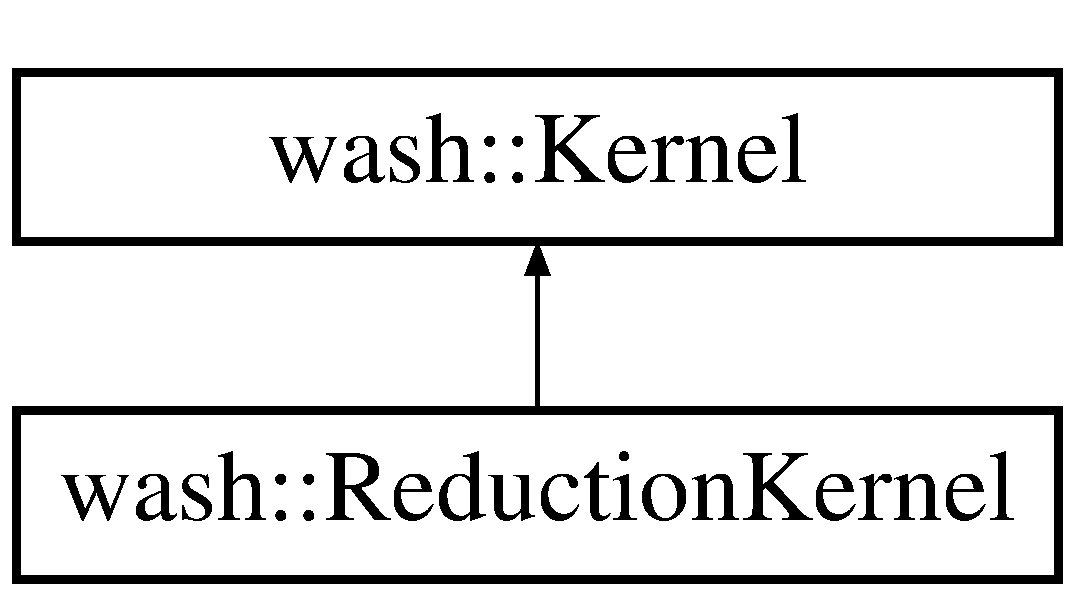
\includegraphics[height=2.000000cm]{classwash_1_1ReductionKernel}
\end{center}
\end{figure}
\subsection*{Public Member Functions}
\begin{DoxyCompactItemize}
\item 
\mbox{\Hypertarget{classwash_1_1ReductionKernel_ab916c2db7332203aed95dbd1adfbdd8e}\label{classwash_1_1ReductionKernel_ab916c2db7332203aed95dbd1adfbdd8e}} 
{\bfseries Reduction\+Kernel} (const Map\+FuncT map\+\_\+func, const Reduce\+FuncT reduce\+\_\+func, const double seed, const std\+::string variable)
\item 
\mbox{\Hypertarget{classwash_1_1ReductionKernel_a3ead90df8748700f40b2e6820e8e7e91}\label{classwash_1_1ReductionKernel_a3ead90df8748700f40b2e6820e8e7e91}} 
virtual void {\bfseries exec} () const override
\item 
\mbox{\Hypertarget{classwash_1_1ReductionKernel_ab916c2db7332203aed95dbd1adfbdd8e}\label{classwash_1_1ReductionKernel_ab916c2db7332203aed95dbd1adfbdd8e}} 
{\bfseries Reduction\+Kernel} (const Map\+FuncT map\+\_\+func, const Reduce\+FuncT reduce\+\_\+func, const double seed, const std\+::string variable)
\item 
\mbox{\Hypertarget{classwash_1_1ReductionKernel_aa06e992c0bc5d3e97fdf7553ad583bf3}\label{classwash_1_1ReductionKernel_aa06e992c0bc5d3e97fdf7553ad583bf3}} 
virtual void {\bfseries exec} () const override
\end{DoxyCompactItemize}


The documentation for this class was generated from the following files\+:\begin{DoxyCompactItemize}
\item 
/dcs/20/u2002000/4th\+Year\+Project/wash/src/wash/wash.\+hpp\item 
/dcs/20/u2002000/4th\+Year\+Project/wash/src/wash/wash.\+cpp\end{DoxyCompactItemize}

\hypertarget{classSedovComputer}{}\section{Sedov\+Computer Class Reference}
\label{classSedovComputer}\index{Sedov\+Computer@{Sedov\+Computer}}
\subsection*{Static Public Member Functions}
\begin{DoxyCompactItemize}
\item 
\mbox{\Hypertarget{classSedovComputer_a5aa65182382334ed24bf803e60967795}\label{classSedovComputer_a5aa65182382334ed24bf803e60967795}} 
static double {\bfseries sedov\+Sol} (const size\+\_\+t dim, const double time, const double eblast, const double omega\+\_\+i, const double gamma\+\_\+i, const double rho0, const double u0, const double p0, const double vel0, const double cs0, const std\+::vector$<$ double $>$ \&r, std\+::vector$<$ double $>$ \&rho, std\+::vector$<$ double $>$ \&p, std\+::vector$<$ double $>$ \&u, std\+::vector$<$ double $>$ \&vel, std\+::vector$<$ double $>$ \&cs)
\end{DoxyCompactItemize}
\subsection*{Static Public Attributes}
\begin{DoxyCompactItemize}
\item 
\mbox{\Hypertarget{classSedovComputer_a3a79b1c2c435337f92488129f15ad323}\label{classSedovComputer_a3a79b1c2c435337f92488129f15ad323}} 
static double {\bfseries rho\+\_\+shock}
\item 
\mbox{\Hypertarget{classSedovComputer_aaca1a1a129526f6861d9c219a025ed56}\label{classSedovComputer_aaca1a1a129526f6861d9c219a025ed56}} 
static double {\bfseries p\+\_\+shock}
\item 
\mbox{\Hypertarget{classSedovComputer_ac8e574be46eb693b095e85c5d157bffb}\label{classSedovComputer_ac8e574be46eb693b095e85c5d157bffb}} 
static double {\bfseries vel\+\_\+shock}
\item 
\mbox{\Hypertarget{classSedovComputer_a597b5c8321e0737b514ddb121844053d}\label{classSedovComputer_a597b5c8321e0737b514ddb121844053d}} 
static double {\bfseries u\+\_\+shock}
\item 
\mbox{\Hypertarget{classSedovComputer_afd12699016e5eb9bc8c2c42ca4fb00bd}\label{classSedovComputer_afd12699016e5eb9bc8c2c42ca4fb00bd}} 
static double {\bfseries cs\+\_\+shock}
\end{DoxyCompactItemize}


The documentation for this class was generated from the following files\+:\begin{DoxyCompactItemize}
\item 
/dcs/20/u2002000/4th\+Year\+Project/wash/src/examples/sedov\+\_\+solution/\mbox{\hyperlink{sedov__computer_8hpp}{sedov\+\_\+computer.\+hpp}}\item 
/dcs/20/u2002000/4th\+Year\+Project/wash/src/examples/sedov\+\_\+solution/\mbox{\hyperlink{sedov__computer_8cpp}{sedov\+\_\+computer.\+cpp}}\end{DoxyCompactItemize}

\hypertarget{classwash_1_1UpdateKernel}{}\section{wash\+:\+:Update\+Kernel Class Reference}
\label{classwash_1_1UpdateKernel}\index{wash\+::\+Update\+Kernel@{wash\+::\+Update\+Kernel}}
Inheritance diagram for wash\+:\+:Update\+Kernel\+:\begin{figure}[H]
\begin{center}
\leavevmode
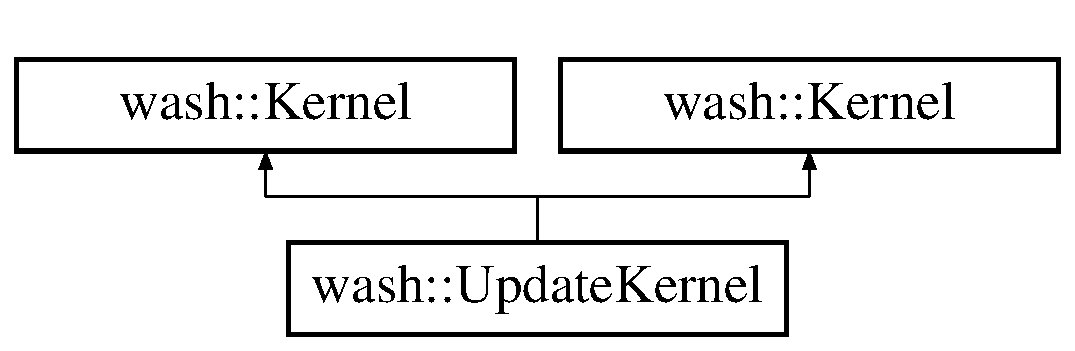
\includegraphics[height=2.000000cm]{classwash_1_1UpdateKernel}
\end{center}
\end{figure}
\subsection*{Public Member Functions}
\begin{DoxyCompactItemize}
\item 
\mbox{\Hypertarget{classwash_1_1UpdateKernel_a2cd95c4f9bcbceff9df7d094f7d7011f}\label{classwash_1_1UpdateKernel_a2cd95c4f9bcbceff9df7d094f7d7011f}} 
{\bfseries Update\+Kernel} (const Update\+FuncT func)
\item 
\mbox{\Hypertarget{classwash_1_1UpdateKernel_a72ec6b0ea453d97708f3fcfd98970366}\label{classwash_1_1UpdateKernel_a72ec6b0ea453d97708f3fcfd98970366}} 
virtual void {\bfseries exec} () const override
\item 
\mbox{\Hypertarget{classwash_1_1UpdateKernel_a2cd95c4f9bcbceff9df7d094f7d7011f}\label{classwash_1_1UpdateKernel_a2cd95c4f9bcbceff9df7d094f7d7011f}} 
{\bfseries Update\+Kernel} (const Update\+FuncT func)
\item 
\mbox{\Hypertarget{classwash_1_1UpdateKernel_a23c7bb181196e107afb1ca4ce9c79137}\label{classwash_1_1UpdateKernel_a23c7bb181196e107afb1ca4ce9c79137}} 
virtual void {\bfseries exec} () const override
\end{DoxyCompactItemize}


The documentation for this class was generated from the following files\+:\begin{DoxyCompactItemize}
\item 
/dcs/20/u2002000/4th\+Year\+Project/wash/src/wash/wash.\+hpp\item 
/dcs/20/u2002000/4th\+Year\+Project/wash/src/wash/wash.\+cpp\end{DoxyCompactItemize}

\hypertarget{classwash_1_1Vec}{}\section{wash\+:\+:Vec$<$ T, dim $>$ Class Template Reference}
\label{classwash_1_1Vec}\index{wash\+::\+Vec$<$ T, dim $>$@{wash\+::\+Vec$<$ T, dim $>$}}
\subsection*{Public Member Functions}
\begin{DoxyCompactItemize}
\item 
\mbox{\Hypertarget{classwash_1_1Vec_a6250ba5f027e9e0e974654136ea7e6ef}\label{classwash_1_1Vec_a6250ba5f027e9e0e974654136ea7e6ef}} 
{\bfseries Vec} (std\+::initializer\+\_\+list$<$ T $>$ l)
\item 
\mbox{\Hypertarget{classwash_1_1Vec_a5927d6caa8489a88b8470fe8bb8779d0}\label{classwash_1_1Vec_a5927d6caa8489a88b8470fe8bb8779d0}} 
T $\ast$ {\bfseries operator\mbox{[}$\,$\mbox{]}} (int i)
\item 
\mbox{\Hypertarget{classwash_1_1Vec_ad8a8863138b26c2b2eae41e11f40e78f}\label{classwash_1_1Vec_ad8a8863138b26c2b2eae41e11f40e78f}} 
\mbox{\hyperlink{classwash_1_1Vec}{Vec}}$<$ T, dim $>$ {\bfseries operator+} (T d)
\item 
\mbox{\Hypertarget{classwash_1_1Vec_a951a842c43b3cf99d60abfe73e53475c}\label{classwash_1_1Vec_a951a842c43b3cf99d60abfe73e53475c}} 
\mbox{\hyperlink{classwash_1_1Vec}{Vec}}$<$ T, dim $>$ {\bfseries operator+} (\mbox{\hyperlink{classwash_1_1Vec}{Vec}}$<$ T, dim $>$ v)
\item 
\mbox{\Hypertarget{classwash_1_1Vec_ac92d90da0a36cdd6b38a8a12e341fa84}\label{classwash_1_1Vec_ac92d90da0a36cdd6b38a8a12e341fa84}} 
void {\bfseries operator+=} (\mbox{\hyperlink{classwash_1_1Vec}{Vec}}$<$ T, dim $>$ v)
\item 
\mbox{\Hypertarget{classwash_1_1Vec_a83a86542f9afb7ea0b5b7b8ab72eb119}\label{classwash_1_1Vec_a83a86542f9afb7ea0b5b7b8ab72eb119}} 
\mbox{\hyperlink{classwash_1_1Vec}{Vec}}$<$ T, dim $>$ {\bfseries operator-\/} (\mbox{\hyperlink{classwash_1_1Vec}{Vec}}$<$ T, dim $>$ v) const
\item 
\mbox{\Hypertarget{classwash_1_1Vec_a972cde51776de1a9efec7ed6ea02f401}\label{classwash_1_1Vec_a972cde51776de1a9efec7ed6ea02f401}} 
\mbox{\hyperlink{classwash_1_1Vec}{Vec}}$<$ T, dim $>$ {\bfseries operator/} (T d)
\item 
\mbox{\Hypertarget{classwash_1_1Vec_a6fc9e30b352c72c7307bd28ee6c0aa72}\label{classwash_1_1Vec_a6fc9e30b352c72c7307bd28ee6c0aa72}} 
\mbox{\hyperlink{classwash_1_1Vec}{Vec}}$<$ T, dim $>$ {\bfseries operator$\ast$} (T d)
\item 
\mbox{\Hypertarget{classwash_1_1Vec_a41de499daf12160b2cf515ce0c9da70f}\label{classwash_1_1Vec_a41de499daf12160b2cf515ce0c9da70f}} 
T {\bfseries magnitude} ()
\item 
\mbox{\Hypertarget{classwash_1_1Vec_a1be26013b6d4f898b8504fc258043400}\label{classwash_1_1Vec_a1be26013b6d4f898b8504fc258043400}} 
T {\bfseries at} (const size\+\_\+t i) const
\item 
\mbox{\Hypertarget{classwash_1_1Vec_aae15a1a2cea7e883e53c2e7f6164710a}\label{classwash_1_1Vec_aae15a1a2cea7e883e53c2e7f6164710a}} 
\mbox{\hyperlink{classwash_1_1Vec}{Vec}}$<$ T, dim $>$ {\bfseries abs} () const
\end{DoxyCompactItemize}


The documentation for this class was generated from the following file\+:\begin{DoxyCompactItemize}
\item 
/dcs/20/u2002000/4th\+Year\+Project/wash/wash\+\_\+vector.\+hpp\end{DoxyCompactItemize}

\hypertarget{classwash_1_1VoidKernel}{}\section{wash\+:\+:Void\+Kernel Class Reference}
\label{classwash_1_1VoidKernel}\index{wash\+::\+Void\+Kernel@{wash\+::\+Void\+Kernel}}


Void \mbox{\hyperlink{classwash_1_1Kernel}{Kernel}} has no arguments/return.  




{\ttfamily \#include $<$kernels.\+hpp$>$}

Inheritance diagram for wash\+:\+:Void\+Kernel\+:\begin{figure}[H]
\begin{center}
\leavevmode
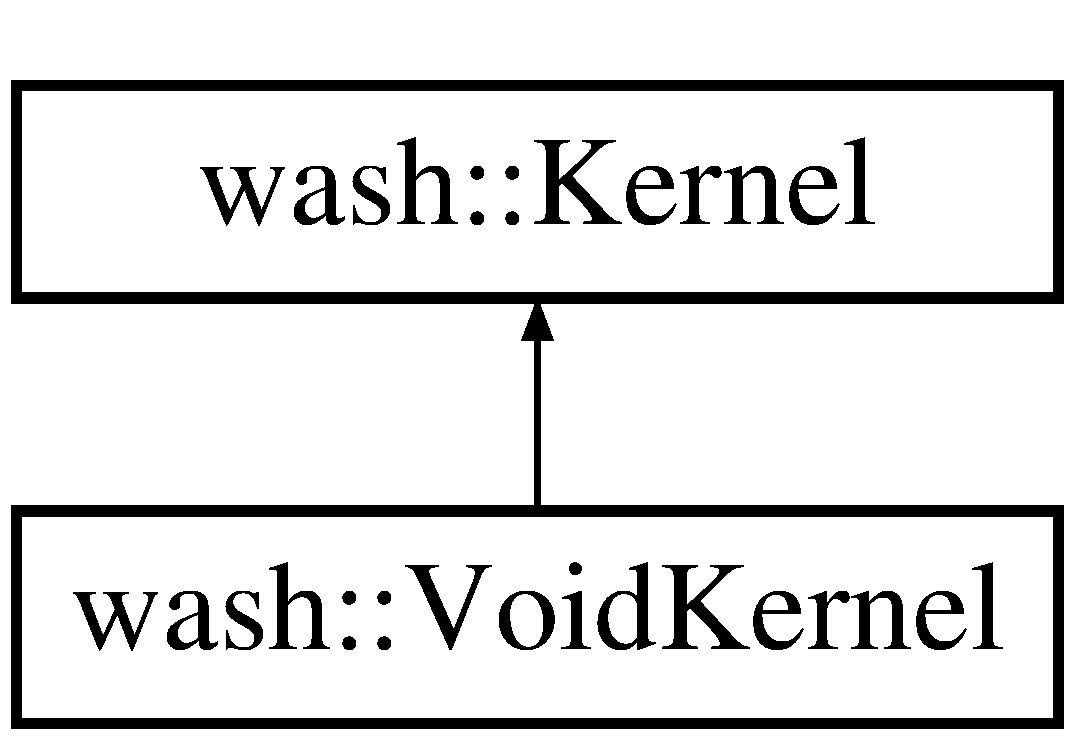
\includegraphics[height=2.000000cm]{classwash_1_1VoidKernel}
\end{center}
\end{figure}
\subsection*{Public Member Functions}
\begin{DoxyCompactItemize}
\item 
\mbox{\Hypertarget{classwash_1_1VoidKernel_abe7159c42c48bf15cf3d69dbf09388dc}\label{classwash_1_1VoidKernel_abe7159c42c48bf15cf3d69dbf09388dc}} 
{\bfseries Void\+Kernel} (const Void\+FuncT func)
\item 
\mbox{\Hypertarget{classwash_1_1VoidKernel_a2a271788509bac47a96dbbecd7fbe90e}\label{classwash_1_1VoidKernel_a2a271788509bac47a96dbbecd7fbe90e}} 
virtual void {\bfseries exec} () const override
\end{DoxyCompactItemize}


\subsection{Detailed Description}
Void \mbox{\hyperlink{classwash_1_1Kernel}{Kernel}} has no arguments/return. 

The documentation for this class was generated from the following files\+:\begin{DoxyCompactItemize}
\item 
/dcs/20/u2002000/4th\+Year\+Project/wash/include/kernels.\+hpp\item 
/dcs/20/u2002000/4th\+Year\+Project/wash/src/impl/cstone/kernels.\+cpp\end{DoxyCompactItemize}

\hypertarget{classwash_1_1WashKernelConsumer}{}\section{wash\+:\+:Wash\+Kernel\+Consumer Class Reference}
\label{classwash_1_1WashKernelConsumer}\index{wash\+::\+Wash\+Kernel\+Consumer@{wash\+::\+Wash\+Kernel\+Consumer}}
Inheritance diagram for wash\+:\+:Wash\+Kernel\+Consumer\+:\begin{figure}[H]
\begin{center}
\leavevmode
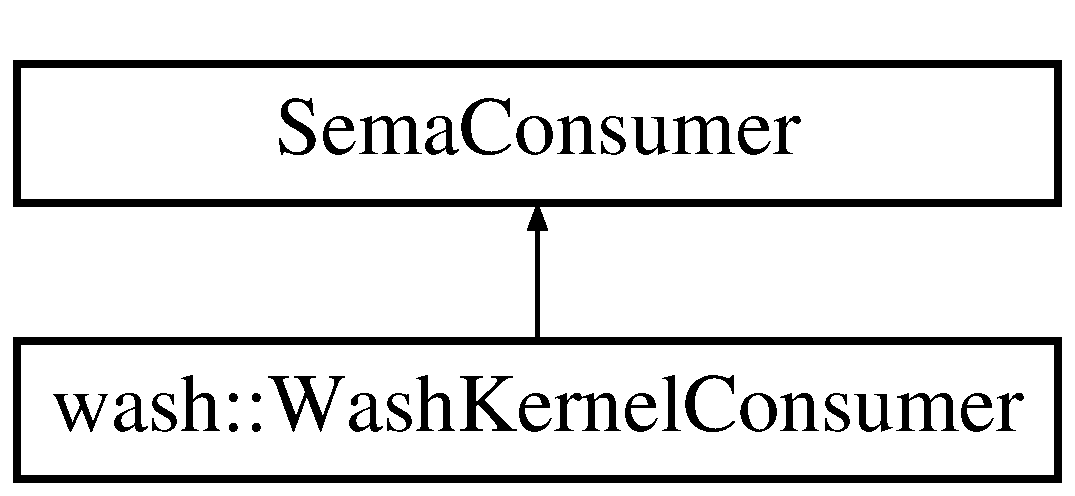
\includegraphics[height=2.000000cm]{classwash_1_1WashKernelConsumer}
\end{center}
\end{figure}
\subsection*{Public Member Functions}
\begin{DoxyCompactItemize}
\item 
\mbox{\Hypertarget{classwash_1_1WashKernelConsumer_a8a3a43dcfdb34cb1891d54e413b707e3}\label{classwash_1_1WashKernelConsumer_a8a3a43dcfdb34cb1891d54e413b707e3}} 
void {\bfseries Initialize\+Sema} (clang\+::\+Sema \&S) override
\item 
\mbox{\Hypertarget{classwash_1_1WashKernelConsumer_a0531ff5c2b5dcb62315a1394c388dbfd}\label{classwash_1_1WashKernelConsumer_a0531ff5c2b5dcb62315a1394c388dbfd}} 
void {\bfseries Forget\+Sema} () override
\item 
\mbox{\Hypertarget{classwash_1_1WashKernelConsumer_a1baaebde57e096b696b446583bfb8f3c}\label{classwash_1_1WashKernelConsumer_a1baaebde57e096b696b446583bfb8f3c}} 
void {\bfseries Handle\+Translation\+Unit} (clang\+::\+A\+S\+T\+Context \&Context) override
\item 
\mbox{\Hypertarget{classwash_1_1WashKernelConsumer_aa62ab9fa6e26322416d3bab549571c05}\label{classwash_1_1WashKernelConsumer_aa62ab9fa6e26322416d3bab549571c05}} 
bool {\bfseries Handle\+Top\+Level\+Decl} (clang\+::\+Decl\+Group\+Ref DG) override
\end{DoxyCompactItemize}


The documentation for this class was generated from the following files\+:\begin{DoxyCompactItemize}
\item 
/dcs/20/u2002000/4th\+Year\+Project/wash/src/gen/kernels.\+hpp\item 
/dcs/20/u2002000/4th\+Year\+Project/wash/src/gen/\mbox{\hyperlink{kernels_8cpp}{kernels.\+cpp}}\end{DoxyCompactItemize}

\hypertarget{classwash_1_1WashKernelsAction}{}\section{wash\+:\+:Wash\+Kernels\+Action Class Reference}
\label{classwash_1_1WashKernelsAction}\index{wash\+::\+Wash\+Kernels\+Action@{wash\+::\+Wash\+Kernels\+Action}}
Inheritance diagram for wash\+:\+:Wash\+Kernels\+Action\+:\begin{figure}[H]
\begin{center}
\leavevmode
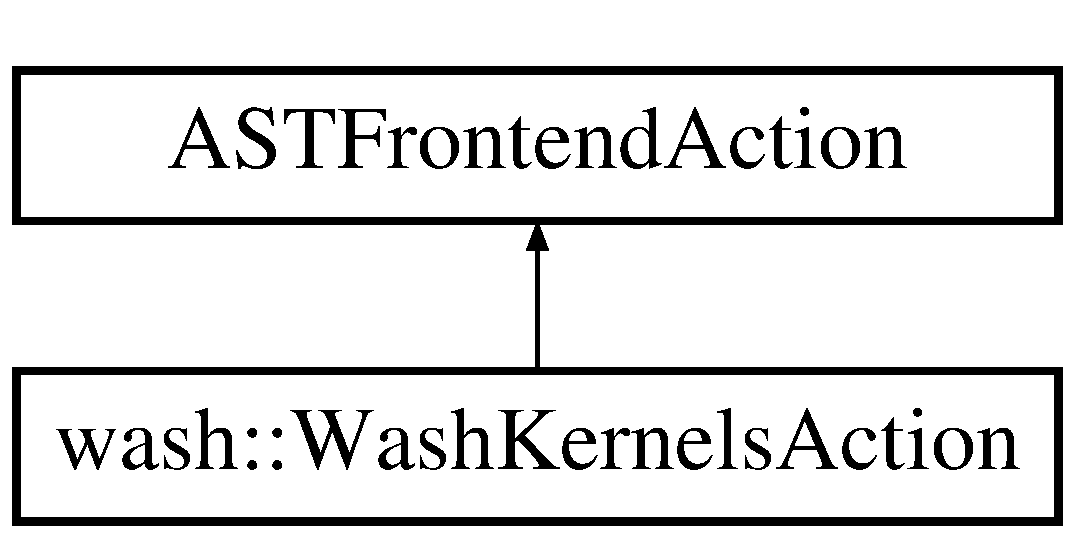
\includegraphics[height=2.000000cm]{classwash_1_1WashKernelsAction}
\end{center}
\end{figure}
\subsection*{Public Member Functions}
\begin{DoxyCompactItemize}
\item 
\mbox{\Hypertarget{classwash_1_1WashKernelsAction_a05069ff0dedbbc1bd149f12b70b8ae44}\label{classwash_1_1WashKernelsAction_a05069ff0dedbbc1bd149f12b70b8ae44}} 
std\+::unique\+\_\+ptr$<$ clang\+::\+A\+S\+T\+Consumer $>$ {\bfseries Create\+A\+S\+T\+Consumer} (clang\+::\+Compiler\+Instance \&Compiler, llvm\+::\+String\+Ref In\+File) override
\end{DoxyCompactItemize}


The documentation for this class was generated from the following file\+:\begin{DoxyCompactItemize}
\item 
/dcs/20/u2002000/4th\+Year\+Project/wash/src/gen/kernels.\+hpp\end{DoxyCompactItemize}

\chapter{File Documentation}
\hypertarget{sedov__computer_8cpp}{}\section{/dcs/20/u2002000/4th\+Year\+Project/wash/src/examples/sedov\+\_\+solution/sedov\+\_\+computer.cpp File Reference}
\label{sedov__computer_8cpp}\index{/dcs/20/u2002000/4th\+Year\+Project/wash/src/examples/sedov\+\_\+solution/sedov\+\_\+computer.\+cpp@{/dcs/20/u2002000/4th\+Year\+Project/wash/src/examples/sedov\+\_\+solution/sedov\+\_\+computer.\+cpp}}
{\ttfamily \#include \char`\"{}sedov\+\_\+computer.\+hpp\char`\"{}}\newline


\subsection{Detailed Description}
\begin{DoxyAuthor}{Author}
Jose A. Escartin \href{mailto:ja.escartin@gmail.com}{\tt ja.\+escartin@gmail.\+com}
\end{DoxyAuthor}
This file is based on the analytical solution presented in S\+P\+H-\/\+E\+XA \href{https://github.com/unibas-dmi-hpc/SPH-EXA}{\tt https\+://github.\+com/unibas-\/dmi-\/hpc/\+S\+P\+H-\/\+E\+XA} 
\hypertarget{sedov__computer_8hpp}{}\section{/dcs/20/u2002000/4th\+Year\+Project/wash/src/examples/sedov\+\_\+solution/sedov\+\_\+computer.hpp File Reference}
\label{sedov__computer_8hpp}\index{/dcs/20/u2002000/4th\+Year\+Project/wash/src/examples/sedov\+\_\+solution/sedov\+\_\+computer.\+hpp@{/dcs/20/u2002000/4th\+Year\+Project/wash/src/examples/sedov\+\_\+solution/sedov\+\_\+computer.\+hpp}}


This class produces 1d solutions for a sedov blast wave propagating through a density gradient\+: rho = rho$\ast$$\ast$(-\/omega) , in planar(1\+D), cylindrical(2\+D) or spherical geometry(3\+D) for the \textquotesingle{}standard\textquotesingle{}, \textquotesingle{}singular\textquotesingle{} and \textquotesingle{}vaccum\textquotesingle{} cases.  


{\ttfamily \#include $<$cmath$>$}\newline
{\ttfamily \#include $<$fstream$>$}\newline
{\ttfamily \#include $<$functional$>$}\newline
{\ttfamily \#include $<$iomanip$>$}\newline
{\ttfamily \#include $<$iostream$>$}\newline
{\ttfamily \#include $<$string$>$}\newline
{\ttfamily \#include $<$variant$>$}\newline
{\ttfamily \#include $<$vector$>$}\newline
{\ttfamily \#include $<$cstdint$>$}\newline
\subsection*{Classes}
\begin{DoxyCompactItemize}
\item 
class \mbox{\hyperlink{classSedovComputer}{Sedov\+Computer}}
\end{DoxyCompactItemize}
\subsection*{Typedefs}
\begin{DoxyCompactItemize}
\item 
using \mbox{\hyperlink{sedov__computer_8hpp_a4b04262b81aa7d31eb5d2f607e2a35de}{Real}} = double
\item 
using \mbox{\hyperlink{sedov__computer_8hpp_ad29765d017498143e4586d5d86b9f32b}{Key\+Type}} = uint64\+\_\+t
\end{DoxyCompactItemize}
\subsection*{Functions}
\begin{DoxyCompactItemize}
\item 
{\footnotesize template$<$class... T, class... Separators$>$ }\\void \mbox{\hyperlink{sedov__computer_8hpp_a774d708554c17cb0fc5b809667cbde62}{write\+Ascii}} (size\+\_\+t first\+Index, size\+\_\+t last\+Index, const std\+::string \&path, bool append, const std\+::vector$<$ std\+::variant$<$ T $\ast$... $>$$>$ \&fields, Separators \&\&... separators)
\item 
void \mbox{\hyperlink{sedov__computer_8hpp_a035d67441548774e0b6cfc00745f61c6}{print\+Help}} (char $\ast$bin\+Name)
\item 
void \mbox{\hyperlink{sedov__computer_8hpp_a14e41e46e8c7a63f4da8dd3f0b392391}{write\+Columns1D}} (const std\+::string \&path)
\end{DoxyCompactItemize}


\subsection{Detailed Description}
This class produces 1d solutions for a sedov blast wave propagating through a density gradient\+: rho = rho$\ast$$\ast$(-\/omega) , in planar(1\+D), cylindrical(2\+D) or spherical geometry(3\+D) for the \textquotesingle{}standard\textquotesingle{}, \textquotesingle{}singular\textquotesingle{} and \textquotesingle{}vaccum\textquotesingle{} cases. 

\begin{DoxyAuthor}{Author}
Jose A. Escartin \href{mailto:ja.escartin@gmail.com}{\tt ja.\+escartin@gmail.\+com}
\begin{DoxyItemize}
\item standard case\+: a nonzero solution extends from the shock to the origin, where the pressure is finite.
\item singular case\+: a nonzero solution extends from the shock to the origin, where the pressure vanishes.
\item vacuum case \+: a nonzero solution extends from the shock to a boundary point, where the density vanishes making the pressure meaningless. \begin{DoxyVerb}   This routine is a C++ conversion of one Fortran code based in these two papers:
   - "Evaluation of the sedov-von neumann-taylor blast wave solution", Jim Kamm, la-ur-00-6055
   - "The sedov self-similiar point blast solutions in nonuniform media", David Book, shock waves, 4, 1, 1994

   Although the ordinary differential equations are analytic, the sedov expressions appear to become singular for
\end{DoxyVerb}
 various combinations of parameters and at the lower limits of the integration range. All these singularies are removable and done so by this routine.
\end{DoxyItemize}
\end{DoxyAuthor}
This file is based on the analytical solution presented in S\+P\+H-\/\+E\+XA \href{https://github.com/unibas-dmi-hpc/SPH-EXA}{\tt https\+://github.\+com/unibas-\/dmi-\/hpc/\+S\+P\+H-\/\+E\+XA}

\begin{DoxyDate}{Date}
2023-\/11-\/30 
\end{DoxyDate}


\subsection{Typedef Documentation}
\mbox{\Hypertarget{sedov__computer_8hpp_ad29765d017498143e4586d5d86b9f32b}\label{sedov__computer_8hpp_ad29765d017498143e4586d5d86b9f32b}} 
\index{sedov\+\_\+computer.\+hpp@{sedov\+\_\+computer.\+hpp}!Key\+Type@{Key\+Type}}
\index{Key\+Type@{Key\+Type}!sedov\+\_\+computer.\+hpp@{sedov\+\_\+computer.\+hpp}}
\subsubsection{\texorpdfstring{Key\+Type}{KeyType}}
{\footnotesize\ttfamily using \mbox{\hyperlink{sedov__computer_8hpp_ad29765d017498143e4586d5d86b9f32b}{Key\+Type}} =  uint64\+\_\+t}

\mbox{\Hypertarget{sedov__computer_8hpp_a4b04262b81aa7d31eb5d2f607e2a35de}\label{sedov__computer_8hpp_a4b04262b81aa7d31eb5d2f607e2a35de}} 
\index{sedov\+\_\+computer.\+hpp@{sedov\+\_\+computer.\+hpp}!Real@{Real}}
\index{Real@{Real}!sedov\+\_\+computer.\+hpp@{sedov\+\_\+computer.\+hpp}}
\subsubsection{\texorpdfstring{Real}{Real}}
{\footnotesize\ttfamily using \mbox{\hyperlink{sedov__computer_8hpp_a4b04262b81aa7d31eb5d2f607e2a35de}{Real}} =  double}



\subsection{Function Documentation}
\mbox{\Hypertarget{sedov__computer_8hpp_a035d67441548774e0b6cfc00745f61c6}\label{sedov__computer_8hpp_a035d67441548774e0b6cfc00745f61c6}} 
\index{sedov\+\_\+computer.\+hpp@{sedov\+\_\+computer.\+hpp}!print\+Help@{print\+Help}}
\index{print\+Help@{print\+Help}!sedov\+\_\+computer.\+hpp@{sedov\+\_\+computer.\+hpp}}
\subsubsection{\texorpdfstring{print\+Help()}{printHelp()}}
{\footnotesize\ttfamily void print\+Help (\begin{DoxyParamCaption}\item[{char $\ast$}]{bin\+Name }\end{DoxyParamCaption})}

\mbox{\Hypertarget{sedov__computer_8hpp_a774d708554c17cb0fc5b809667cbde62}\label{sedov__computer_8hpp_a774d708554c17cb0fc5b809667cbde62}} 
\index{sedov\+\_\+computer.\+hpp@{sedov\+\_\+computer.\+hpp}!write\+Ascii@{write\+Ascii}}
\index{write\+Ascii@{write\+Ascii}!sedov\+\_\+computer.\+hpp@{sedov\+\_\+computer.\+hpp}}
\subsubsection{\texorpdfstring{write\+Ascii()}{writeAscii()}}
{\footnotesize\ttfamily template$<$class... T, class... Separators$>$ \\
void write\+Ascii (\begin{DoxyParamCaption}\item[{size\+\_\+t}]{first\+Index,  }\item[{size\+\_\+t}]{last\+Index,  }\item[{const std\+::string \&}]{path,  }\item[{bool}]{append,  }\item[{const std\+::vector$<$ std\+::variant$<$ T $\ast$... $>$$>$ \&}]{fields,  }\item[{Separators \&\&...}]{separators }\end{DoxyParamCaption})}

\mbox{\Hypertarget{sedov__computer_8hpp_a14e41e46e8c7a63f4da8dd3f0b392391}\label{sedov__computer_8hpp_a14e41e46e8c7a63f4da8dd3f0b392391}} 
\index{sedov\+\_\+computer.\+hpp@{sedov\+\_\+computer.\+hpp}!write\+Columns1D@{write\+Columns1D}}
\index{write\+Columns1D@{write\+Columns1D}!sedov\+\_\+computer.\+hpp@{sedov\+\_\+computer.\+hpp}}
\subsubsection{\texorpdfstring{write\+Columns1\+D()}{writeColumns1D()}}
{\footnotesize\ttfamily void write\+Columns1D (\begin{DoxyParamCaption}\item[{const std\+::string \&}]{path }\end{DoxyParamCaption})}


\hypertarget{finder_8cpp}{}\section{/dcs/20/u2002000/4th\+Year\+Project/wash/src/gen/finder.cpp File Reference}
\label{finder_8cpp}\index{/dcs/20/u2002000/4th\+Year\+Project/wash/src/gen/finder.\+cpp@{/dcs/20/u2002000/4th\+Year\+Project/wash/src/gen/finder.\+cpp}}


Implements the Find Wash Function funtionality.  


{\ttfamily \#include \char`\"{}finder.\+hpp\char`\"{}}\newline


\subsection{Detailed Description}
Implements the Find Wash Function funtionality. 

\begin{DoxyAuthor}{Author}
jamesm2w 
\end{DoxyAuthor}
\begin{DoxyVersion}{Version}
0.\+1 
\end{DoxyVersion}
\begin{DoxyDate}{Date}
2023-\/12-\/14
\end{DoxyDate}
\begin{DoxyCopyright}{Copyright}
Copyright (c) 2023 
\end{DoxyCopyright}

\hypertarget{finder_8hpp}{}\section{/dcs/20/u2002000/4th\+Year\+Project/wash/src/gen/finder.hpp File Reference}
\label{finder_8hpp}\index{/dcs/20/u2002000/4th\+Year\+Project/wash/src/gen/finder.\+hpp@{/dcs/20/u2002000/4th\+Year\+Project/wash/src/gen/finder.\+hpp}}


Find Wash Function is a small tool/plugin which scans through program source code and reports a) wash function declarations and b) wash function calls.  


{\ttfamily \#include \char`\"{}clang/\+A\+S\+T/\+A\+S\+T.\+h\char`\"{}}\newline
{\ttfamily \#include \char`\"{}clang/\+A\+S\+T/\+A\+S\+T\+Consumer.\+h\char`\"{}}\newline
{\ttfamily \#include \char`\"{}clang/\+A\+S\+T/\+Recursive\+A\+S\+T\+Visitor.\+h\char`\"{}}\newline
{\ttfamily \#include \char`\"{}clang/\+Frontend/\+Compiler\+Instance.\+h\char`\"{}}\newline
{\ttfamily \#include \char`\"{}clang/\+Frontend/\+Frontend\+Action.\+h\char`\"{}}\newline
{\ttfamily \#include \char`\"{}clang/\+Tooling/\+Tooling.\+h\char`\"{}}\newline
{\ttfamily \#include \char`\"{}clang/\+Frontend/\+Frontend\+Plugin\+Registry.\+h\char`\"{}}\newline
{\ttfamily \#include \char`\"{}iostream\char`\"{}}\newline
\subsection*{Classes}
\begin{DoxyCompactItemize}
\item 
class \mbox{\hyperlink{classFindWashFunctionVisitor}{Find\+Wash\+Function\+Visitor}}
\item 
class \mbox{\hyperlink{classFindWashFunctionConsumer}{Find\+Wash\+Function\+Consumer}}
\end{DoxyCompactItemize}


\subsection{Detailed Description}
Find Wash Function is a small tool/plugin which scans through program source code and reports a) wash function declarations and b) wash function calls. 

\begin{DoxyAuthor}{Author}
jamesm2w 
\end{DoxyAuthor}
\begin{DoxyVersion}{Version}
0.\+1 
\end{DoxyVersion}
\begin{DoxyDate}{Date}
2023-\/12-\/14
\end{DoxyDate}
\begin{DoxyCopyright}{Copyright}
Copyright (c) 2023 
\end{DoxyCopyright}

\hypertarget{finder__plugin_8cpp}{}\section{/dcs/20/u2002000/4th\+Year\+Project/wash/src/gen/finder\+\_\+plugin.cpp File Reference}
\label{finder__plugin_8cpp}\index{/dcs/20/u2002000/4th\+Year\+Project/wash/src/gen/finder\+\_\+plugin.\+cpp@{/dcs/20/u2002000/4th\+Year\+Project/wash/src/gen/finder\+\_\+plugin.\+cpp}}


Implements the Find Wash Function as a plugin for clang compiler.  


{\ttfamily \#include \char`\"{}finder.\+hpp\char`\"{}}\newline
\subsection*{Classes}
\begin{DoxyCompactItemize}
\item 
class \mbox{\hyperlink{classFindWashFunctionsPlugin}{Find\+Wash\+Functions\+Plugin}}
\begin{DoxyCompactList}\small\item\em Implements the plugin through using the already defined behaviour of the frontent action. \end{DoxyCompactList}\end{DoxyCompactItemize}


\subsection{Detailed Description}
Implements the Find Wash Function as a plugin for clang compiler. 

\begin{DoxyAuthor}{Author}
jamesm2w 
\end{DoxyAuthor}
\begin{DoxyVersion}{Version}
0.\+1 
\end{DoxyVersion}
\begin{DoxyDate}{Date}
2023-\/12-\/14
\end{DoxyDate}
\begin{DoxyCopyright}{Copyright}
Copyright (c) 2023 
\end{DoxyCopyright}

\hypertarget{finder__tool_8cpp}{}\section{/dcs/20/u2002000/4th\+Year\+Project/wash/src/gen/finder\+\_\+tool.cpp File Reference}
\label{finder__tool_8cpp}\index{/dcs/20/u2002000/4th\+Year\+Project/wash/src/gen/finder\+\_\+tool.\+cpp@{/dcs/20/u2002000/4th\+Year\+Project/wash/src/gen/finder\+\_\+tool.\+cpp}}


Runs the Find Wash Function as a standalone clang tool on passed in code.  


{\ttfamily \#include \char`\"{}finder.\+hpp\char`\"{}}\newline
\subsection*{Classes}
\begin{DoxyCompactItemize}
\item 
class \mbox{\hyperlink{classFindWashFunctionAction}{Find\+Wash\+Function\+Action}}
\end{DoxyCompactItemize}
\subsection*{Functions}
\begin{DoxyCompactItemize}
\item 
\mbox{\Hypertarget{finder__tool_8cpp_a3c04138a5bfe5d72780bb7e82a18e627}\label{finder__tool_8cpp_a3c04138a5bfe5d72780bb7e82a18e627}} 
int {\bfseries main} (int argc, char $\ast$$\ast$argv)
\end{DoxyCompactItemize}


\subsection{Detailed Description}
Runs the Find Wash Function as a standalone clang tool on passed in code. 

\begin{DoxyAuthor}{Author}
jamesm2w 
\end{DoxyAuthor}
\begin{DoxyVersion}{Version}
0.\+1 
\end{DoxyVersion}
\begin{DoxyDate}{Date}
2023-\/12-\/14
\end{DoxyDate}
\begin{DoxyCopyright}{Copyright}
Copyright (c) 2023 
\end{DoxyCopyright}

\hypertarget{inspect_8cpp}{}\section{/dcs/20/u2002000/4th\+Year\+Project/wash/src/gen/inspect.cpp File Reference}
\label{inspect_8cpp}\index{/dcs/20/u2002000/4th\+Year\+Project/wash/src/gen/inspect.\+cpp@{/dcs/20/u2002000/4th\+Year\+Project/wash/src/gen/inspect.\+cpp}}


Inspecting the contents of Wa\+SH C++ files.  


{\ttfamily \#include \char`\"{}inspect.\+hpp\char`\"{}}\newline
\subsection*{Functions}
\begin{DoxyCompactItemize}
\item 
\mbox{\Hypertarget{inspect_8cpp_a3c04138a5bfe5d72780bb7e82a18e627}\label{inspect_8cpp_a3c04138a5bfe5d72780bb7e82a18e627}} 
int {\bfseries main} (int argc, char $\ast$$\ast$argv)
\item 
std\+::ostream \& \mbox{\hyperlink{inspect_8cpp_a7bfba47bce91c57d0de28179bad2ad1b}{operator$<$$<$}} (std\+::ostream \&stream, const C\+X\+String \&str)
\begin{DoxyCompactList}\small\item\em Helper to output Clang strings nicely. \end{DoxyCompactList}\end{DoxyCompactItemize}


\subsection{Detailed Description}
Inspecting the contents of Wa\+SH C++ files. 

\begin{DoxyAuthor}{Author}
jamesm2w 
\end{DoxyAuthor}
\begin{DoxyVersion}{Version}
0.\+1 
\end{DoxyVersion}
\begin{DoxyDate}{Date}
2023-\/12-\/14
\end{DoxyDate}
\begin{DoxyCopyright}{Copyright}
Copyright (c) 2023 
\end{DoxyCopyright}


\subsection{Function Documentation}
\mbox{\Hypertarget{inspect_8cpp_a7bfba47bce91c57d0de28179bad2ad1b}\label{inspect_8cpp_a7bfba47bce91c57d0de28179bad2ad1b}} 
\index{inspect.\+cpp@{inspect.\+cpp}!operator$<$$<$@{operator$<$$<$}}
\index{operator$<$$<$@{operator$<$$<$}!inspect.\+cpp@{inspect.\+cpp}}
\subsubsection{\texorpdfstring{operator$<$$<$()}{operator<<()}}
{\footnotesize\ttfamily std\+::ostream\& operator$<$$<$ (\begin{DoxyParamCaption}\item[{std\+::ostream \&}]{stream,  }\item[{const C\+X\+String \&}]{str }\end{DoxyParamCaption})}



Helper to output Clang strings nicely. 


\begin{DoxyParams}{Parameters}
{\em stream} & \\
\hline
{\em str} & \\
\hline
\end{DoxyParams}
\begin{DoxyReturn}{Returns}
std\+::ostream\& 
\end{DoxyReturn}

\hypertarget{kernels_8cpp}{}\section{/dcs/20/u2002000/4th\+Year\+Project/wash/src/gen/kernels.cpp File Reference}
\label{kernels_8cpp}\index{/dcs/20/u2002000/4th\+Year\+Project/wash/src/gen/kernels.\+cpp@{/dcs/20/u2002000/4th\+Year\+Project/wash/src/gen/kernels.\+cpp}}


Implementations for the kernel plugin/tool.  


{\ttfamily \#include \char`\"{}kernels.\+hpp\char`\"{}}\newline


\subsection{Detailed Description}
Implementations for the kernel plugin/tool. 

\begin{DoxyAuthor}{Author}
jamesm2w 
\end{DoxyAuthor}
\begin{DoxyVersion}{Version}
0.\+1 
\end{DoxyVersion}
\begin{DoxyDate}{Date}
2023-\/12-\/18
\end{DoxyDate}
\begin{DoxyCopyright}{Copyright}
Copyright (c) 2023 
\end{DoxyCopyright}

\hypertarget{read__ascii_8cpp}{}\section{/dcs/20/u2002000/4th\+Year\+Project/wash/src/io/read\+\_\+ascii.cpp File Reference}
\label{read__ascii_8cpp}\index{/dcs/20/u2002000/4th\+Year\+Project/wash/src/io/read\+\_\+ascii.\+cpp@{/dcs/20/u2002000/4th\+Year\+Project/wash/src/io/read\+\_\+ascii.\+cpp}}


Reads in an ascii plaintext file into the simulation as a checkpoint.  


{\ttfamily \#include \char`\"{}ascii.\+hpp\char`\"{}}\newline


\subsection{Detailed Description}
Reads in an ascii plaintext file into the simulation as a checkpoint. 

\begin{DoxyAuthor}{Author}
James Macer-\/\+Wright 
\end{DoxyAuthor}
\begin{DoxyVersion}{Version}
0.\+1 
\end{DoxyVersion}
\begin{DoxyDate}{Date}
2023-\/11-\/15
\end{DoxyDate}
\begin{DoxyCopyright}{Copyright}
Copyright (c) 2023 
\end{DoxyCopyright}

\hypertarget{read__hdf5_8cpp}{}\section{/dcs/20/u2002000/4th\+Year\+Project/wash/src/io/read\+\_\+hdf5.cpp File Reference}
\label{read__hdf5_8cpp}\index{/dcs/20/u2002000/4th\+Year\+Project/wash/src/io/read\+\_\+hdf5.\+cpp@{/dcs/20/u2002000/4th\+Year\+Project/wash/src/io/read\+\_\+hdf5.\+cpp}}


Reads in a H\+D\+F5 file with the intention of constructing a simulation state from which to continue.  


{\ttfamily \#include \char`\"{}hdf5.\+hpp\char`\"{}}\newline


\subsection{Detailed Description}
Reads in a H\+D\+F5 file with the intention of constructing a simulation state from which to continue. 

\begin{DoxyAuthor}{Author}
James Macer-\/\+Wright 
\end{DoxyAuthor}
\begin{DoxyVersion}{Version}
0.\+1 
\end{DoxyVersion}
\begin{DoxyDate}{Date}
2023-\/11-\/15
\end{DoxyDate}
\begin{DoxyCopyright}{Copyright}
Copyright (c) 2023
\end{DoxyCopyright}
Occasionally, we might want to stop the computation of a simulation for various reasons eventually we will then want to restart the simulation starting from where we left of. 
\hypertarget{write__ascii_8cpp}{}\section{/dcs/20/u2002000/4th\+Year\+Project/wash/src/io/write\+\_\+ascii.cpp File Reference}
\label{write__ascii_8cpp}\index{/dcs/20/u2002000/4th\+Year\+Project/wash/src/io/write\+\_\+ascii.\+cpp@{/dcs/20/u2002000/4th\+Year\+Project/wash/src/io/write\+\_\+ascii.\+cpp}}


Writes the simulation data to an ascii plaintext file in C\+SV format.  


{\ttfamily \#include $<$fstream$>$}\newline
{\ttfamily \#include \char`\"{}ascii.\+hpp\char`\"{}}\newline
\subsection*{Namespaces}
\begin{DoxyCompactItemize}
\item 
 \mbox{\hyperlink{namespacewash}{wash}}
\begin{DoxyCompactList}\small\item\em T\+O\+DO\+: Consider having this as a private header in W\+I\+S\+B/\+W\+S2\+S\+T/etc implementations. \end{DoxyCompactList}\item 
 \mbox{\hyperlink{namespacewash_1_1io}{wash\+::io}}
\end{DoxyCompactItemize}
\subsection*{Functions}
\begin{DoxyCompactItemize}
\item 
int \mbox{\hyperlink{namespacewash_1_1io_ab29d891bfd64999f5ffb3aa5b13c5b22}{wash\+::io\+::write\+\_\+ascii}} (const I\+O\+Manager \&io, const Simulation\+Data \&sim\+\_\+data, size\+\_\+t iter)
\begin{DoxyCompactList}\small\item\em Write A\+S\+C\+II Output. \end{DoxyCompactList}\end{DoxyCompactItemize}


\subsection{Detailed Description}
Writes the simulation data to an ascii plaintext file in C\+SV format. 

\begin{DoxyAuthor}{Author}
James Macer-\/\+Wright 
\end{DoxyAuthor}
\begin{DoxyVersion}{Version}
0.\+1 
\end{DoxyVersion}
\begin{DoxyDate}{Date}
2023-\/11-\/15
\end{DoxyDate}
\begin{DoxyCopyright}{Copyright}
Copyright (c) 2023 
\end{DoxyCopyright}

\hypertarget{write__hdf5_8cpp}{}\section{/dcs/20/u2002000/4th\+Year\+Project/wash/src/io/write\+\_\+hdf5.cpp File Reference}
\label{write__hdf5_8cpp}\index{/dcs/20/u2002000/4th\+Year\+Project/wash/src/io/write\+\_\+hdf5.\+cpp@{/dcs/20/u2002000/4th\+Year\+Project/wash/src/io/write\+\_\+hdf5.\+cpp}}


Write out the simulation state serially to a H\+D\+F5 file.  


{\ttfamily \#include \char`\"{}hdf5.\+hpp\char`\"{}}\newline


\subsection{Detailed Description}
Write out the simulation state serially to a H\+D\+F5 file. 

\begin{DoxyAuthor}{Author}
James Macer-\/\+Wright 
\end{DoxyAuthor}
\begin{DoxyVersion}{Version}
0.\+1 
\end{DoxyVersion}
\begin{DoxyDate}{Date}
2023-\/11-\/15
\end{DoxyDate}
\begin{DoxyCopyright}{Copyright}
Copyright (c) 2023
\end{DoxyCopyright}
Periodically we want to write out the simulation data to a file to inspect the intermediate values of particles \& properties. This can be achieved with a number of different backend technologies, H\+D\+F5 is one which supports parallelism with M\+PI.

As well, H\+D\+F5 formats can be read by visualisation software such as S\+P\+La\+SH which was built for visualising S\+PH simulation data.

We expect H\+D\+F5 to be built and present on the system for this use. 
\hypertarget{write__hdf5__dump_8cpp}{}\section{/dcs/20/u2002000/4th\+Year\+Project/wash/src/io/write\+\_\+hdf5\+\_\+dump.cpp File Reference}
\label{write__hdf5__dump_8cpp}\index{/dcs/20/u2002000/4th\+Year\+Project/wash/src/io/write\+\_\+hdf5\+\_\+dump.\+cpp@{/dcs/20/u2002000/4th\+Year\+Project/wash/src/io/write\+\_\+hdf5\+\_\+dump.\+cpp}}


Writes out to a H\+D\+F5 file in a similar format to sedov. With a singular dump file contianing each iteration as a separate group, with attributes controlling time\+Step and iteration no.  


{\ttfamily \#include \char`\"{}hdf5.\+hpp\char`\"{}}\newline


\subsection{Detailed Description}
Writes out to a H\+D\+F5 file in a similar format to sedov. With a singular dump file contianing each iteration as a separate group, with attributes controlling time\+Step and iteration no. 

\begin{DoxyAuthor}{Author}
James Macer-\/\+Wright $<$$>$ 
\end{DoxyAuthor}
\begin{DoxyVersion}{Version}
0.\+1 
\end{DoxyVersion}
\begin{DoxyDate}{Date}
2023-\/12-\/02 
\end{DoxyDate}

%--- End generated contents ---

% Index
\backmatter
\newpage
\phantomsection
\clearemptydoublepage
\addcontentsline{toc}{chapter}{Index}
\printindex

\end{document}
